\documentclass{article}
\usepackage[utf8]{inputenc}
\usepackage{parskip}
\usepackage{tikz}
\usetikzlibrary{decorations.markings, calc, arrows.meta, hobby, intersections, decorations.pathreplacing, calligraphy, patterns}
\usepackage{pifont}
\usepackage[labelfont=bf, textfont=it]{caption}
\usepackage[left=3.5cm,right=3.5cm]{geometry}
\usepackage{physics}
\usepackage{mathtools}
\usepackage{amssymb}
\usepackage{amsfonts}
\usepackage{amsthm}
\usepackage{cancel}
\usepackage{esint}
\usepackage{graphicx}
\usepackage{tgpagella}
\usepackage[english]{babel}
\usepackage{xparse}
\usepackage{enumitem}
\usepackage{pgfplots}
\pgfplotsset{width=10cm,compat=1.9}

\setlist[enumerate]{label=(\arabic*)}
\setlist[itemize]{label=\ding{226}}

\usepackage{hyperref}
\everymath{\displaystyle}

\allowdisplaybreaks[2]

\newcommand{\halfarrow}[2]{%
  \path (#1) -- (#2) coordinate[pos=0.25] (Pstart) coordinate[pos=0.75] (Pend);
  \draw[-{Stealth}, thick, black] (Pstart) -- (Pend);
}

\newcommand{\ddx}{\dd{x}}
\newcommand{\ddy}{\dd{y}}
\newcommand{\ddz}{\dd{z}}
\newcommand{\ddzeta}{\dd{\zeta}}
\newcommand{\ddt}{\dd{t}}
\newcommand{\supp}{\operatorname{supp}}
\newcommand{\Log}{\mathrm{Log}}
\newcommand{\Arg}{\mathrm{Arg}}
\newcommand{\Aut}{\mathrm{Aut}}

\newtheorem{theorem}{Theorem}[section]
\newtheorem{corollary}{Corollary}[theorem]
\newtheorem{lemma}{Lemma}[section]
\theoremstyle{remark}
\newtheorem{example}{Example}[subsection]
\theoremstyle{definition}
\newtheorem{definition}{Definition}[section]
\theoremstyle{remark}
\newtheorem*{remark}{Remark}
\providecommand*{\lemmaautorefname}{Lemma}
\providecommand*{\definitionautorefname}{Definition}
\providecommand*{\corollaryautorefname}{Corollary}
\providecommand*{\exampleautorefname}{Example}
\numberwithin{equation}{section}
\numberwithin{figure}{section}
\DeclarePairedDelimiter{\paren}{(}{)}
\let\parendefault\paren
\renewcommand{\paren}{\parendefault*}
\DeclarePairedDelimiter{\brackets}{[}{]}
\let\bracketsdefault\brackets
\renewcommand{\brackets}{\bracketsdefault*}
\DeclarePairedDelimiter\ceil{\lceil}{\rceil}
\let\ceildefault\ceil
\renewcommand{\ceil}{\ceildefault*}
\DeclarePairedDelimiter\floor{\lfloor}{\rfloor}
\let\floordefault\floor
\renewcommand{\floor}{\floordefault*}

\NewDocumentCommand{\cbraces}{m g}{\ensuremath{\left\lbrace#1\IfNoValueTF{#2}{}{\,\middle|\,#2}\right\rbrace}}

\newcommand{\riemannsphere}{\widehat{\mathbb{C}}}
\newcommand{\chpref}[1]{\hyperref[#1]{\S\,\ref*{#1}}}

\title{Complex Analysis}
\author{Slipper King}
\date{May 2025}
\begin{document}
\maketitle
\tableofcontents
\section{Prerequisites}
\subsection{Topological Preliminaries}
We will provide a rough, informal notion of important topological concepts tailored specifically towards complex analysis.
\begin{definition}[Accumulation Point]\label{def:accumulationpoint}
    A point \(z\in\mathbb{C}^n\) is an \textit{accumulation point} of \(X\) if for any open set \(U\) containing \(z\), \((U\setminus\{z\})\cap X\neq\emptyset\)
\end{definition}
\begin{definition}[Closure]\label{def:closure}
    For a set \(X\in\mathbb{C}^n\), define the \textit{closure} of \(X\), or \(\overline{X}\) to be the intersection of all closed sets containing \(X\). In other words, it is the union of \(X\) and its accumulation points.
\end{definition}
\begin{definition}[Interior]\label{def:interior}
    For a set \(X\in\mathbb{C}^n\), the \textit{interior} of \(X\), denoted \(X^\circ\), is the union of all open sets contained in \(X\), or the set of points \(z\in\mathbb{C}^n\) such that there exists an open neighborhood of \(z\) that is fully contained in \(X\).
\end{definition}
\begin{definition}[Compact Set]\label{def:compactsets}
    A set \(X\in\mathbb{C}^n\) is compact if and only if \(X\) is closed and bounded.
\end{definition}
\begin{definition}[Cover of a Set]
    A cover \(\mathcal{C}\) of a set \(X\) is a collection of sets \(\cbraces{U_n}\) such that \[\bigcup_{n\in\mathbb{N}}U_n\supseteq X.\] A cover is \textit{open} if every set in the collection is open.
\end{definition}
\begin{theorem}[Bolzano--Weierstrass Theorem]\label{thm:bolzanoweierstrass}
    Every infinite subset \(A\) of a compact set \(X\subset\mathbb{C}^n\) has an accumulation point in \(X\).
\end{theorem}
\begin{proof}
    Since \(X\) is bounded, there exists a closed cube \(Q\subset\mathbb{C}^n\) such that \(A\subseteq X\subset Q\).

    Bisect \(Q_0=Q\) into \(2^{2n}\) congruent sub-cubes. Since \(A\) is infinite and the sub-cubes are finite in number, at least one of the sub-cubes contains infinitely many points of \(A\), and choose one to be \(Q_1\).

    Bisect \(Q_1\) into \(2^{2n}\) sub-cubes, and choose a sub-cube \(Q_2\subset Q_1\) that contains infinitely many points of \(A\). We then obtain the recursive sequence \[Q_0\supset Q_1 \supset Q_2\supset\cdots.\]

    Because the side lengths shrink to zero and the cubes are nested, the intersection
    \[\bigcap_{k=0}^{\infty} Q_k\]
    consists of exactly one point. Call this point \(z_\infty\in\mathbb{C}^n\).

    For each \(k\), \(Q_k\) contains infinitely many points of \(A\). Because the side length of \(Q_k\) tends to zero, for any \(\varepsilon>0\), \(\exists N\in\mathbb{N}\) such that \(\forall k\geq N\), \(Q_k\subset B^n(z_\infty,\varepsilon)\) where \(B^n(a,r)\subset\mathbb{C}^n\) is the \(n\)-dimensional \textit{ball} with radius \(r\) centered at \(a=\paren{a_1,a_2,\ldots,a_n}\in\mathbb{C}^n\), or \[B^n(a,r)=\cbraces{\qty(z_1,z_2,\ldots,z_n)\in\mathbb{C}^n}{\sum_{j=1}^n\abs{z_j-a_j}^2<r^2}.\]
    Then, \(B^n(z_\infty, \varepsilon)\) also contains infinitely many points of \(A\). Therefore, \(z_\infty\) is an accumulation point of \(A\).

    We now show that \(z_\infty\in X\). Suppose for contradiction that \(z_\infty\notin X\). Since \(X\) is closed, \(\mathbb{C}^n\setminus X\) is open, and \(\exists\delta>0\) such that \[B^n(z_\infty,\delta)\subset\mathbb{C}^n\setminus X.\] But then, for sufficiently large \(k\), we have \(Q_k \subset B^n(z_\infty, \delta)\), and hence \(Q_k\cap X=\emptyset\). This contradicts the construction of \(Q_k\), which ensures that \(Q_k\) contains infinitely many points of \(A \subset X\).
\end{proof}
\begin{theorem}[Heine-Borel Theorem]\label{thm:heineborel}
    A set \(X\in\mathbb{C}^n\) is compact if and only if every open cover has a finite subcover.
\end{theorem}
\begin{proof}
    We will first show that any set satisfying the condition is compact.

    First we will show that \(X\) is bounded. Suppose that \(\forall R>0\), \(\exists z\in X\) where \(\norm{z}>R\). Consider the collection of open sets \[\mathcal{U}=\{B^n(0,k)\mid k\in\mathbb{N}\}.\] \(\mathcal{U}\) forms an open cover of \(X\). Then by the assumption, there exists a finite subcover in \(\mathcal{U}\), namely \(\{B^n(0,k_1),\ldots,B^n(0,k_m)\}\) which covers \(X\). Then, \[X\subseteq\bigcup_{i=1}^mB^n(0,k_i)=B^n(0,\max(k_1,\ldots k_m)).\] By contradiction, \(X\) must be bounded.

    \(X\) must also be a closed set. For the sake of contradiction, assume that there exists a point \(z_0\in\overline{X}\setminus X\). Since \(z_0\notin X\), the following open collection of sets covers \(X\):
    \[\mathcal{U}=\left\{\mathbb{C}^n\setminus\overline{B^n\qty(z_0,\frac{1}{k})}\;\middle|\; \forall k\in\mathbb{N}\right\}.\]
    There then exists a finite subcover \(\mathcal{C}=\left\{\mathbb{C}^n\setminus\overline{B^n\qty(z_0,\frac{1}{k_i})}\;\middle|\; i=1,2,\ldots,m\right\}\). Then, \[X\subseteq\mathbb{C}^n\setminus\overline{B^n\qty(z_0,\frac{1}{\max(k_1,\ldots,k_m)})},\]
    and that \(X\cap\overline{B^n\qty(z_0,\frac{1}{\max(k_1,\ldots,k_m)})}=\emptyset\). However, by the definition of the accumulation point, every open neighborhood of the accumulation point must intersect \(X\). Therefore, by contradiction, \(X\) is closed.

    We then prove the converse. By the assumption that \(X\) is bounded, \(\exists R>0\) such that the \(X\) is contained within the closed cube \[Q=\left\{z\;\middle|\; z\in\mathbb{C}^n, \max_{i\in\{1,\ldots,n\}}\abs{\Re(z_i)}\le R,\max_{i\in\{1,\ldots,n\}}\abs{\Im(z_i)}\le R\right\}.\]

    Assume that there exists an infinite open cover \(\mathcal{U}\) of \(X\) without finite subcovering. Bisect \(Q_0=Q\) into \(2^{2n}\) sub-cubes (for real and complex parts). Choose \(Q_1\) such that \(Q_1\cup X\) has no finite subcover of \(\mathcal{U}\). Under the previous assumptions, this is possible since if every \(\text{sub-cube}\cap X\) had finite subcovering, then \(Q_0\cap X=X\) would have finite subcovering. Similarly, choose \(Q_2\) by bisecting \(Q_1\) in a similar way, and recursively obtain a sequence of cubes:
    \[Q_0\supset Q_1\supset Q_2\supset\ldots\]
    Since the side length of each cube tends to 0, \(\bigcap_{i=0}^\infty Q_i\) consists of a single point \(z_{\infty}\in\mathbb{C}^n\). By the Bolzano-Weierstrass Theorem (\autoref{thm:bolzanoweierstrass}), because \(\forall i\in\mathbb{N}\), \(Q_i\cap X\neq\emptyset\), select a point \(z_{i}\in Q_i\cap X\), forming a sequence \({z_k}\in X\) convergent to \(z_\infty\in X\) as \(X\) is closed. Therefore, \(\exists U\in\mathcal{U}\) where \(z_\infty\in U\). Since \(U\) is open, \(\exists\varepsilon>0\) such that \(B^n(z_\infty,\varepsilon)\subset U\). \(\exists N\in\mathbb{N}\) such that \(\forall k>N\), \(Q_k\subset B^n(z_\infty,\varepsilon)\). Then taking the intersection with \(X\) on both sides, \[Q_k\cap X\subseteq B^n(z_\infty,\varepsilon)\cap X\subset U.\] Our original assumption said that for every \(k\), \(Q_k\cap X\) has no finite subcovering. However, \(U\) covers \(Q_k\cap X\), which is a single open set that covers a nonempty subset. Therefore by contradiction, every open cover has finite subcovering.
\end{proof}
\begin{definition}[Support of a Function]\label{def:support}
    For a set \(X\) and a function \(f:X\to\mathbb{C}\), the support, denoted as \(\supp(f)=\overline{\{z\in X\mid f(z)\neq 0\}}\), is the closure of the set for which \(f\) is nonzero.
\end{definition}
\begin{remark}
    We are primarily concerned when the support of a function is compact, or if the support is bounded. Smooth functions that are compactly supported are also called \textit{bump functions}.
\end{remark}
\subsection{Calculus}
Since complex analysis is essentially the theory of calculus on complex functions, it is only natural that generalizations are made on classical formulas in calculus for real functions.

It is well known that a function \(f:(a,b)\to\mathbb{R}\) is differentiable at a point \(x\in(a,b)\) if the limit \[\lim_{h\to0}\frac{f(x+h)-f(x)}{h}\] exists, and the value of this limit is the derivative of \(f(x)\), denoted by \(f'(x)\) or \(\frac{\dd{f}}{\ddx}\). The value \(\dd{f}=f'(x)\ddx\) is the differential of \(f(x)\). Partition \([a,b]\) into \(a=x_0<x_1<x_2<\cdots<x_n=b\). Such that the length of the intervals \([x_i,x_{i-1}]\) tends to 0 as \(n\to\infty\). If for any such partition, the sum \[\sum_{i=1}^n f(\xi_i)(x_i-x_{i-1})\] tends to the same value \(\forall\xi_i\in[x_{i-1},x_i]\), then the function can be roughly said to be integrable over \([a,b]\). The full details of Riemann integrability relate to the upper and lower Riemann sums and will not be discussed here. The value of this sum is denoted by \[\int_a^bf(x)\dd{x}.\] The following theorems are the fundamental results of classical calculus:
\begin{theorem}[Fundamental Theorem of Calculus, Differential Form]
    Let \(f(x)\) be a function continuous over \([a,b]\). For \(x\in[a,b]\), define
    \[\Phi(x)=\int_a^xf(t)\dd{t}.\]
    Then \(\Phi(x)\) is differentiable over \([a,b]\), \(\Phi'(x)=f(x)\), and \(\dd{\Phi(x)}=f(x)\dd{x}\).
\end{theorem}
\begin{theorem}[Fundamental Theorem of Calculus, Integral Form]
    Let \(\Phi(x)\) be a function differentiable over \([a,b]\). Let \(f(x)=\Phi'(x)\) over \([a,b]\). Then,
    \[\int_a^xf(t)\dd{t}=\Phi(x)-\Phi(a).\]
\end{theorem}
The two forms of the theorem show that differentiation and integration are inverse operations to each other. Operations performed for differentiating oftentimes have a corresponding inverse operation that can be done for integrating. For instance, \[\dv{(f(x)\pm g(x))}{x}=\dv{f(x)}{x}\pm\dv{g(x)}{x}\] corresponds to \[\int(f(x)\pm g(x))\ddx=\int f(x)\ddx\pm\int g(x)\ddx,\]
and \[\dv{x}(f(x)g(x))=f'(x)g(x)+f(x)g'(x)\] corresponds to \[\int f(x)g'(x)\ddx=f(x)g(x)-\int f'(x)g(x)\ddx,\] and \[\dv{f(g(x))}{x}=\dv{f(g)}{g}\cdot\dv{g(x)}{x}\] corresponds to \[\int_a^bf(g(x))g'(x)\ddx=\int_{g(a)}^{g(b)}f(u)\dd{u}.\] Another correspondence is the Mean Value Theorem:
\begin{theorem}[Mean Value Theorem, Differential Form]
    If \(f(x)\) is differentiable over \([a,b]\), then \(\exists c\in[a,b]\) such that \[f(b)-f(a)=f'(c)(b-a).\]
\end{theorem}
\begin{theorem}[Mean Value Theorem, Integral Form]
    If \(f(x)\) is continuous over \([a,b]\), then \(\exists \xi\in[a,b]\) such that \[\int_a^bf(x)\ddx=f(\xi)(b-a).\]
\end{theorem}
A curve is a one-dimensional manifold embedded within a higher dimensional space. They can be parameterized with a vector \(\va{F}(t)=\mqty(P(t)\\Q(t)\\R(t))\) of one parameter. In the complex plane, a curve is a complex-valued function \(\gamma(t)\) for a real parameter \(\alpha\leq t\leq\beta\). A curve is \textit{closed} if \(\gamma(\alpha)=\gamma(\beta)\). It is \textit{smooth} if it is continuously differentiable, and its direction is defined to be the direction as \(t\) increases. If it is smooth everywhere except at a finite number of points, it is \textit{piecewise smooth}. If it is of finite length, then the curve is said to be \textit{rectifiable}. Piecewise smooth curves are rectifiable. A curve is \textit{simple} if it is simple (non self-intersecting), or if \(\gamma\paren{t_1}=\gamma\paren{t_2}\) implies that \(t_1=t_2\). A simple closed curve is also called a \textit{Jordan curve}.
\begin{theorem}[Jordan Curve Theorem]\label{thm:jordancurve}
    Let \(\gamma\) be a Jordan curve in \(\mathbb{R}^2\). Then the set \(\mathbb{R}^2\setminus\gamma\) consists of exactly two connected subsets. One of them is the interior, denoted by \(\mathrm{int}(\gamma)\), and is a bounded set, while the other is the exterior, denoted by \(\mathrm{ext}(\gamma)\), which is unbounded. Both of the two sets share the common boundary \(\gamma\).
\end{theorem}
The theorem above seems trivial, but has a complicated rigorous proof in topology. The theorem can also be stated on \(\mathbb{C}\) instead of \(\mathbb{R}^2\). For a region \(U\), the boundary is denoted \(\partial U\). If the region bounded by any closed curve in \(U\) also lies in \(U\), then it is a \textit{simply connected} region. A connected region that is not simply connected is multiply connected. A region bound by 2 non-intersecting Jordan curves is doubly connected, and a region bound by \(n\) non-intersecting Jordan curves is traditionally known as \(n\)-connected (the modern topological definition differs). Lastly, any closed curve can degenerate to a single point or slit.

Generalizations of the differential and integral exist for multivariate functions. The partial differentials of \(f(x,y,z)\), \(\pdv{f}{x}\ddx\), \(\pdv{f}{y}\ddy\), and \(\pdv{f}{z}\ddz\) sum up to form the total differential, denoted by \(\dd{f}\). An important result in multivariable calculus allows the calculation of the derivatives of a definite integral with respect to its parameter.
\begin{theorem}[Leibniz Integral Rule]\label{thm:leibnizintegralrule}
    Let \(I\subset\mathbb{R}\) be open, and let \(a:I\to\mathbb{R}\) and \(b:I\to\mathbb{R}\) be differentiable on \(I\) such that \(\forall x\in I\), \(a(x)<b(x)\). Let \[U=\cbraces{(x,t)\in I\times\mathbb{R}}{a(x)\leq t\leq b(x)}.\] Suppose \(f(x,t)\) is a real-valued function on \(U\) such that \(f(x,t)\) and \(\pdv{f}{x}(x,t)\) are continuous on the set \(U\). Then the function \[F(x)=\int_{a(x)}^{b(x)}f(x,t)\dd{t}\] is differentiable on \(I\), and
    \[\dv{F}{x}=\int_{a(x)}^{b(x)}\pdv{f}{x}(x,t)\dd{t} + f(x,b(x))\dv{b}{x} - f(x,a(x))\dv{a}{x}.\]
\end{theorem}
Four main classical theorems exist, relating a function and its line integral in 2 and 3 dimensions, line and surface integrals in 2 and 3 dimensions, and the surface and volume integrals in 3 dimensions:
\begin{theorem}[Gradient Theorem]\label{thm:gradient}
    Let \(C\) be an oriented smooth curve in \(\mathbb{R}^3\) with boundary points \(A\) to \(B\). Then
    \[\int_C\pdv{f}{x} \ddx+\pdv{f}{y}\ddy+\pdv{f}{z}\ddz=f(B)-f(A).\]
\end{theorem}
\begin{theorem}[Green's Theorem]\label{thm:realgreen}
    Let \(U\) be a positively oriented, multiply connected region in \(\mathbb{R}^2\) with a piecewise smooth oriented boundary \(\partial U\). For \(P(x,y),Q(x,y)\in C^1\paren{\overline{U}}\),
    \[\oint_{\partial U} P\ddx+Q\ddy=\iint_U\paren{\pdv{Q}{x}-\pdv{P}{y}}\ddx\ddy.\]
\end{theorem}
\begin{theorem}[Stokes' Theorem]\label{thm:kelvinstokes}
    Let \(S\subset\mathbb{R}^3\) be a positively oriented, smooth surface with a positively oriented boundary curve \(\partial S\). Let \(P(x,y,z),Q(x,y,z),R(x,y,z)\in C^1\paren{\overline{S}}\). Then,
    \begin{align*}
        \oint_{\partial S}P\ddx+Q\ddy+R\ddz & =\iint_S\left(\pdv{R}{y}-\pdv{Q}{z}\right)\ddy\ddz+\left(\pdv{P}{z}-\pdv{R}{x}\right)\dd{z}\ddx+\left(\pdv{Q}{x}-\pdv{P}{y}\right)\ddx\ddy.
    \end{align*}
\end{theorem}
\begin{theorem}[Gauss' Theorem]\label{thm:divergencegauss}
    Let \(V\) be a positively oriented region in \(\mathbb{R}^3\) with a smooth, positively oriented boundary surface \(\partial V\). Let \(P(x,y,z),Q(x,y,z),R(x,y,z)\in C^1\paren{\overline{V}}\). Then,
    \[\oiint_{\partial V}P\ddy\ddz+Q\ddz\ddx+R\ddx\ddy=\iiint_V\left(\pdv{P}{x}+\pdv{Q}{y}+\pdv{R}{z}\right)\ddx\ddy\ddz.\]
\end{theorem}
In 3-dimensional \(\mathbb{R}^3\) space, define a scalar valued function to be a 0-form, a linear combination of \(\ddx\), \(\dd{y}\), and \(\dd{z}\) to be a 1-form, and a linear combination of \(\dd{y}\wedge\dd{z}\), \(\dd{z}\wedge\ddx\), and \(\dd{x}\wedge\dd{y}\) to be a 2-form, and \(\ddx\wedge\dd{y}\wedge\dd{z}\) to be a 3-form, where \(\wedge\) denotes an anti-commutative and associative product, where for any two differential forms \(\omega_1\) and \(\omega_2\)
\[\omega_1\wedge\omega_2=-\omega_2\wedge\omega_1.\]
Then consequently, for any differential form \(\omega\), \[\omega\wedge\omega=0.\]
We can generalize the operator \(\dd\) to increase the degree of a differential form. For instance,
\[df=\pdv{f}{x}\ddx+\pdv{f}{y}\dd{y}+\pdv{f}{z}\dd{z},\]
which is the definition of the total differential. For a 1-form in 3-dimensional space, \(\omega_1=P\ddx+Q\dd{y}+R\dd{z}\), we can define the exterior derivative in a similar way: \begin{align*}
    \dd{\omega_1} & =\dd{P}\wedge\ddx+\dd{Q}\wedge\dd{y}+\dd{R}\wedge\dd{z}                                                                                                    \\
                  & =\left(\pdv{P}{x}\ddx+\pdv{P}{y}\dd{y}+\pdv{P}{z}\dd{z}\right)\wedge\ddx                                                                                   \\
                  & \qquad+\left(\pdv{Q}{x}\ddx+\pdv{Q}{y}\dd{y}+\pdv{Q}{z}\dd{z}\right)\wedge\ddy                                                                             \\
                  & \qquad\qquad+\left(\pdv{R}{x}\ddx+\pdv{R}{y}\dd{y}+\pdv{R}{z}\dd{z}\right)\wedge\dd{z}                                                                     \\
                  & =\left(\pdv{R}{y}-\pdv{Q}{z}\right)\dd{y}\wedge\dd{z}+\left(\pdv{P}{z}-\pdv{R}{x}\right)\dd{z}\wedge\ddx+\left(\pdv{Q}{x}-\pdv{P}{y}\right)\ddx\wedge\ddy.
\end{align*}
Similarly, we can differentiate a 2-form \(\omega=P\ddy\wedge\dd{z}+Q\ddz\wedge\ddx+R\ddx\wedge\ddy\) to get:
\[\left(\pdv{P}{x}+\pdv{Q}{y}+\pdv{R}{z}\right)\ddx\wedge\ddy\wedge\ddz.\]
The two results above resemble the curl and divergence of \(\mqty(P\\Q\\R)\). A differential form \(\omega\) is \textit{closed} if \(\dd{\omega}=0\), and is exact if there exists \(\eta\) such that \(\omega=\dd{\omega}\).
\begin{lemma}[Poincaré's Lemma]\label{lemma:poincare}
    For any differential form \(\omega\) on an open, contractible set \(U\subseteq\mathbb{R}^n\), if \(\omega\) is closed, then it is also exact.
\end{lemma}
It is true that for any set \(U\subseteq \mathbb{R}^n\), regardless of contractibility, that for a differential form \(\omega\) defined on \(U\), \(\dd\dd\omega=0\). In other words, all exact differential forms are closed.

With the same analogy, the above result means that if \(\omega\) is a 0-form, then \(\curl(\grad\omega)=0\), and if \(\omega\) is a 1-form, \(\div(\curl{v})=0\), where \(v\) is the vector of the coefficients of the basis differential forms of \(\omega\) (there are no correlations for higher degree forms since in 3-dimensional space, the highest degree possible for any differential form is 3).

Then, the Fundamental Theorem of Calculus, the Gradient Theorem, Green's, Stokes', and Gauss' Theorems can be generalized into:
\begin{theorem}[Stokes--Cartan Theorem]\label{thm:stokescartan}
    For an oriented smooth \(n\)-dimensional compact manifold \(M\) with boundary \(\partial M\), for a smooth differential \((n-1)\)-form \(\omega\) over \(\overline{M}\), \[\int_M\dd{\omega}=\int_{\partial M}\omega.\]
\end{theorem}
A portion of calculus is dedicated to rigorously defining concepts such as limits, continuity, integrability, etc. The most widely used definition of a finite limit of a function is the language of \(\varepsilon\)--\(\delta\), which states:
\begin{definition}[Epsilon--Delta]\label{def:epsilondelta}
    Let \(f:U\to\mathbb{R}\) be a function defined over an open set \(U\subseteq\mathbb{R}\) such that \(a\) is an accumulation point of \(U\). We say that \(\lim_{x\to a}f(x)=L\) if for every \(\varepsilon > 0\), there exists \(\delta > 0\) such that for all \(x\in U\) with \(0<|x-a|<\delta\), we have \(|f(x)-L|<\varepsilon\).

    Similarly, we define the \textit{right-handed limit} \(\lim_{x\to a^+}f(x)=L\) if for every \(\varepsilon>0\), there exists \(\delta>0\) such that for all \(x\in U\) with \(0<x-a<\delta\), we have \(|f(x)-L|<\varepsilon\).

    Likewise, the \textit{left-hand limit} \(\lim_{x\to a^-}f(x)=L\) exists if for every \(\varepsilon>0\), there exists \(\delta>0\) such that for all \(x\in U\) with \(-\delta<x-a<0\), we have \(|f(x)-L|<\varepsilon\).
\end{definition}
We also have the definition of the limit of a sequence:
\begin{definition}[Epsilon--N]\label{def:epsilonn}
    Let \(\qty{a_n}_{n\in\mathbb{N}}\subset\mathbb{R}\) be a sequence. If \(\exists a_\infty\in\mathbb{R}\) such that \(\forall\varepsilon>0\), \(\exists N\in\mathbb{N}\) such that \(\forall n>N\), \(\abs{a_n-a_\infty}<\varepsilon\), then \(\qty{a_n}\) \textit{converges} to \(a_\infty\).
\end{definition}
\begin{theorem}[Cauchy Criterion]\label{thm:cauchycriterionsequenceconvergence}
    Let \(\qty{a_n}_{n\in\mathbb{N}}\subset\mathbb{R}\) be a sequence. Then \(\qty{a_n}\) is convergent if and only if \(\forall\varepsilon>0\), \(\exists N\in\mathbb{N}\) such that \(\forall n,m>N\), \(\abs{a_n-a_m}<\varepsilon\).
\end{theorem}
\begin{proof}
    Assume \(\qty{a_n}\) is convergent. Then \(\forall\varepsilon>0\), \(\exists N\in\mathbb{N}\) such that \(\forall n,m>N\), \(\abs{a_n-a_\infty}<\frac{\varepsilon}{2}\) and \(\abs{a_m-a_\infty}<\frac{\varepsilon}{2}\) for some \(a_\infty\in\mathbb{R}\). It follows that \[\abs{a_n-a_m}\leq\abs{a_n-a_\infty}+\abs{a_m-a_\infty}=\varepsilon.\]

    Conversely, \(\qty{a_n}\) is bounded (fixing \(N\), \(\forall n>N\), \(\abs{a_n-a_{N+1}}<\varepsilon\)). By the Bolzano--Weierstrass Theorem (\autoref{thm:bolzanoweierstrass}), \(\qty{a_n}\) has a convergent subsequence \(\qty{a_{n_k}}_{k\in\mathbb{N}}\) converging to \(a_\infty\). Therefore, \(\forall\varepsilon>0\), \(\exists N\in\mathbb{N}\) and \(\exists M\in\mathbb{N}\) such that \(\forall k>M\), \(n_k>N\), and \(\forall n>N\), \(\abs{a_n-a_{n_k}}<\frac{\varepsilon}{2}\) and \(\abs{a_{n_k}-a_\infty}<\frac{\varepsilon}{2}\). Then \[\abs{a_n-a_\infty}\leq\abs{a_n-a_{n_k}}+\abs{a_{n_k}-a_\infty}<\varepsilon.\] Hence, \(\qty{a_n}\) converges to \(a_\infty\).
\end{proof}
\begin{definition}[Limit Superior]\label{def:limsup}
    For a number sequence \(\qty{a_n}\subset\mathbb{R}\), if \(\exists a\in\mathbb{R}\) such that:
    \begin{enumerate}
        \item \(\forall\varepsilon>0\), \(\exists N\in\mathbb{N}\) such that \(\forall n>N\), \(a_n<a+\varepsilon\),
        \item \(\forall\varepsilon>0\), \(\forall N\in\mathbb{N}\), \(\exists n>N\) such that \(a_n>a-\varepsilon\),
    \end{enumerate}
    then the \textit{superior limit} of \(\qty{a_n}\) is \(a\), denoted by \(\varlimsup_{n\to\infty}a_n=\limsup_{n\to\infty}a_n=a\).
\end{definition}
\begin{definition}[Limit Inferior]\label{def:liminf}
    For a number sequence \(\qty{a_n}\subset\mathbb{R}\), if \(\exists a\in\mathbb{R}\) such that:
    \begin{enumerate}
        \item \(\forall\varepsilon>0\), \(\exists N\in\mathbb{N}\) such that \(\forall n>N\), \(a_n>a-\varepsilon\),
        \item \(\forall\varepsilon>0\), \(\forall N\in\mathbb{N}\), \(\exists n>N\) such that \(a_n<a+\varepsilon\),
    \end{enumerate}
    then the \textit{inferior limit} of \(\qty{a_n}\) is \(a\), denoted by \(\varliminf_{n\to\infty}a_n=\liminf_{n\to\infty}a_n=a\).
\end{definition}
\begin{lemma}
    A number sequence \(\qty{a_n}\) is convergent if and only if \(\varlimsup_{n\to\infty} a_n=\varliminf_{n\to\infty}a_n\).
\end{lemma}
\begin{proof}
    We first prove that \(a=\lim_{n\to\infty}a_n\) implies \(\varlimsup_{n\to\infty}a_n=\varliminf_{n\to\infty}a_n=a\).
    By \autoref{def:epsilonn}, \(\forall\varepsilon>0\), \(\exists N\in\mathbb{N}\) such that \(\forall n>N\), \[\abs{a_n-a}<\varepsilon\Longleftrightarrow a-\varepsilon<a_n<a+\varepsilon.\]
    Then from the first conditions of \autoref{def:limsup} and \autoref{def:liminf}, we get that \(\varlimsup_{n\to\infty}a_n\geq a\) and \(\varliminf_{n\to\infty} a_n\leq a\). By the second conditions, we get \(\varlimsup_{n\to\infty}a_n\leq a\) and \(\varliminf_{n\to\infty} a_n\geq a\). Therefore, \[\varlimsup_{n\to\infty}a_n=\varliminf_{n\to\infty}a_n.\]

    For the converse, assume \(\varlimsup_{n\to\infty}a_n=\varliminf_{n\to\infty}a_n\). Since \(\exists N_1\in\mathbb{N}\) such that \(\forall n>N_1\), \(a_n<a+\varepsilon\). \(\exists N_2\in\mathbb{N}\) such that \(\forall n>N_2\), \(a_n>a-\varepsilon\). Then \(\forall n>\max\qty(N_1, N_2)\), \(\qty|a_n-a|<\varepsilon\), as expected.
\end{proof}
\begin{definition}[Continuity]\label{def:continuity}
    A function \(f:U \to \mathbb{R}\), defined on an open set \(U \subseteq \mathbb{R}\) containing a point \(a \in U\), is said to be continuous at \(a\) if and only if \[\lim_{x\to a}f(x)=f(a).\]
\end{definition}
\begin{theorem}\label{thm:continuousfunctionboundedoncompact}
    Any continuous function on a compact set \(U\) is bounded on \(U\).
\end{theorem}
\begin{proof}
    Suppose for the sake of contradiction that \(f:U\to\mathbb{R}\) is continuous and unbounded on compact \(U\). Then for each \(n\in\mathbb{N}\), there exists \(x_n\in U\) such that \(|f(x_n)|>n\). The sequence \(\cbraces{x_n}\) lies in \(U\), which is compact, so by the Bolzano--Weierstrass Theorem (\autoref{thm:bolzanoweierstrass}), \(\cbraces{x_n}\) has an accumulation point in \(U\). In other words, there exists a convergent subsequence \(\cbraces{x_{n_k}}\) with \(\lim_{k\to\infty} x_{n_k}\in U\).

    Since \(f\) is continuous, \(\lim_{k\to\infty}f\qty(x_{n_k})=f\qty(\lim_{k\to\infty}x_{n_k})\), which is defined because \(\lim_{k\to\infty} x_{n_k}\in U\). However, this contradicts \(\qty|f\paren{x_{n_k}}|>n_k\to\infty\), hence \(f\) must be bounded on \(U\).
\end{proof}
\begin{theorem}[Extreme Value Theorem]\label{thm:extremevalue}
    A continuous function \(f(x)\) over a compact set \(U\) attains its infimum and supremum in \(U\).
\end{theorem}
\begin{proof}
    Assume that \(f\) never attains its supremum \(M\in U\). Then, \(f(x)<M\). Define the auxiliary function \(\psi(x)=\frac{1}{M-f(x)}\), which is strictly positive and continuous as the denominator never reaches 0. By \autoref{thm:continuousfunctionboundedoncompact}, \(\psi(x)\) is bounded with some value of \(\mu>0\) satisfying \(\psi(x)\leq\mu\). \(f(x)\) also has the representation \(M-\frac{1}{\psi(x)}\), and therefore, \[f(x)\leq M-\frac{1}{\mu},\] which means that \(M\) is not the supremum. Similarly, assume that \(f\) never attains its infimum \(m\in Us\). Then \(f(x)>m\). Let \(\psi(x)=\frac{1}{f(x)-m}\), which is strictly positive and continuous as the denominator never reaches 0. By \autoref{thm:continuousfunctionboundedoncompact}, \(\psi(x)\) is bounded with some value of \(\mu>0\) satisfying \(\psi(x)\leq\mu\). \(f(x)\) also has the representation \(m+\frac{1}{\psi(x)}\), and therefore, \[f(x)\geq m+\frac{1}{\mu},\] which means that \(m\) is not the infimum.
\end{proof}
\begin{definition}[Uniform Continuity]\label{def:uniformcontinuity}
    A function \(f:U\to\mathbb{R}\), defined on a set \(U\subseteq\mathbb{R}\), is uniformly continuous if and only if \(\forall\varepsilon>0\), \(\exists\delta>0\) such that \(\forall x,y\in U\) where \(|x-y|<\delta\), \(\abs{f(x)-f(y)}<\varepsilon\).
\end{definition}
\begin{example}
    The function \(f(x)=\frac{1}{x}\) is not uniformly continuous over \((0,1)\).
\end{example}
\begin{proof}
    If \(\exists\varepsilon>0\) such that \(\forall\delta>0\), \(\exists x,y\in(0,1)\) such that \(|x-y|<\delta\) and \(\abs{f(x)-f(y)}\geq\varepsilon\), then \(f(x)\) is not uniformly continuous over \((0,1)\).

    Let \(\varepsilon=1\) and \[x=\frac{1}{n},\quad y=\frac{1}{n+1}.\] Then \(\forall\delta>0\), \(\exists n>1\) where \(\abs{x-y}<\delta\), since \(\lim_{n\to\infty}\left|x-y\right|=0\). Additionally, \(\abs{f(x)-f(y)}=1\geq\varepsilon\). This satisfies the negation, and thus, \(f(x)=\frac{1}{x}\) is not uniformly continuous over \((0,1)\).
\end{proof}
\begin{lemma}\label{lemma:uniformcontinuousovercompactset}
    A continuous function over a compact set \(U\) is uniformly continuous over \(U\).
\end{lemma}
\begin{proof}
    Suppose for contradiction that \(f:U\to\mathbb{R}\) is continuous but not uniformly continuous on compact \(U\). Then \(\exists\varepsilon>0\) such that \(\forall\delta>0\), \(\exists x,y\in U\) with \(|x-y|<\delta\) and \(|f(x)-f(y)|\geq\varepsilon\).

    In particular, \(\forall n\in\mathbb{N}\), let \(\delta=\frac{1}{n}\). Then \(\exists x_n,y_n\in U\) such that \(|x_n-y_n|<\frac{1}{n}\) and \(|f(x_n)-f(y_n)|\geq\varepsilon\). Since \(U\) is compact, the sequence \(\cbraces{x_n}\) has a convergent subsequence \(x_{n_k}\to x_{n_\infty}\in U\). Because \(\qty|x_{n_k}-y_{n_k}|<\frac{1}{n_k}\to 0\), we also have \(y_{n_k}\to x_{n_\infty}\).

    By continuity, \(f(x_{n_k})\to f\paren{x_{n_\infty}}\) and \(f(y_{n_k})\to f\paren{x_{n_\infty}}\), so \(\qty|f(x_{n_k})-f(y_{n_k})|\to 0\), contradicting \(\qty|f(x_{n_k})-f(y_{n_k})|\geq\varepsilon\). Therefore, \(f\) is uniformly continuous on \(U\).
\end{proof}
\begin{definition}
    A function \(f\) is Lipschitz continuous over \(U\) if \(\exists M\in\mathbb{R}_{\geq0}\) such that \(\forall x,y \in U\), \(|f(x)-f(y)| \leq M|x-y|\). The smallest possible \(M\) satisfying the above condition is known as the Lipschitz constant.
\end{definition}
Lipschitz continuity is an important concept in real analysis and the theory of differential equations. It is a strong form of uniform continuity.
\begin{lemma}
    All Lipschitz continuous functions on \(U\) are uniformly continuous on \(U\).
\end{lemma}
\begin{proof}
    Let \(M>0\) be the Lipschitz constant. Then \(\forall \varepsilon>0\), let \(\delta=\frac{\varepsilon}{M}\). It then follows that \(\forall x,y\in U\) such that \(\abs{x-y}<\delta\), \(\abs{f(x)-f(y)}\leq M|x-y|<\varepsilon\).
\end{proof}
\begin{lemma}\label{lemma:c1lipschitz}
    A \(C^1\) function on a compact set \(U\) is Lipschitz continuous on \(U\).
\end{lemma}
\begin{proof}
    Let \(f:U\to\mathbb{R}\) be \(C^1\). By \autoref{thm:continuousfunctionboundedoncompact}, since \(U\) is compact and \(f'\) is continuous, \(\exists M>0\) such that \(\forall x\in U\), \(|f'(x)|\leq M\).

    By the Mean Value Theorem, \(\forall x,y\in U\), \(\exists c\) between \(x\) and \(y\) such that \(f(x)-f(y)=f'(c)(x-y)\). Then, \(|f(x)-f(y)|=|f'(c)||x-y|\leq M|x-y|\), which means \(f\) is Lipschitz continuous with Lipschitz constant less than or equal to \(M\).
\end{proof}
\section{Complex Prerequisites}
\subsection{The Complex Plane}
All complex numbers form a field that extends the real number field. A complex number \(\alpha+i\beta\) can be visualized on a rectangular plane as the point \((\alpha,\beta)\), with two axes: the real axis and the imaginary axis. It is well known that any complex number also has the polar form \(re^{i\theta}=r\paren{\cos\theta+i\sin\theta}\).

The infinity point, \(\infty\), extends \(\mathbb{C}\) with \(\riemannsphere=\mathbb{C}\cup\{\infty\}\). \(\forall a\in\mathbb{C}\), \(a+\infty=\infty+a=\infty\). \(\forall b\in\mathbb{C}\setminus\{0\}\), \(b\cdot\infty=\infty\cdot b=\infty\) and \(\frac{a}{\infty}=0\).

Let \(S^2=\left\{\paren{x_1,x_2,x_3}\in\mathbb{R}\,\middle|\,x_1^2+x_2^2+x_3^2=1\right\}\). There exists a \textit{stereographic projection} of \(S^2\) onto \(\riemannsphere\). For every point other than \((0,0,1)\), there is a corresponding complex number \begin{equation}\label{eq:riemannsphereformula1}
    z=\frac{x_1+ix_2}{1-x_3}.
\end{equation}
This correspondence between \(\mathbb{C}\) and \(S^2\setminus\left\{(0,0,1)\right\}\) is injective. In fact, the inverse can be solved for:
\[\abs{z}^2=\frac{1-x_3^2}{\paren{1-x_3}^2}=\frac{1+x_3}{1-x_3},\]
which results in \[x_3=\frac{\abs{z}^2-1}{\abs{z}^2+1},\]
and consequently,
\[x_1=\Re\paren{z}\paren{1-x_3}=\frac{z+\overline{z}}{\abs{z}^2+1},\quad x_2=\Im\paren{z}\paren{1-x_3}=\frac{z-\overline{z}}{i\abs{z}^2+i}.\]
By letting \(\infty\) correspond to \(\paren{0,0,1}\), the bijection is complete. The sphere \(S^2\) is also called the \textit{Riemann sphere}. The region given by the disk \(\abs{z}<1\) is given by \(x_3<0\), and the region \(\abs{z}>1\) is given by \(x_3>0\). 

We will now give a geometric visualization of this projection. Let \(z=x+iy\). Then we obtain that \(x=\frac{x_1}{1-x_3}\) and \(y=\frac{x_2}{1-x_3}\). Therefore, \[x:y:1=x_1:x_2:1-x_3.\]
It follows that the points \(\mqty(0\\0\\0)\), \(\mqty(x\\y\\1)\), and \(\mqty(x_1\\x_2\\1-x_3)\) are collinear in \(\mathbb{R}^3\). Under the linear map \(\mathbf{v}\mapsto\mqty(\dmat[0]{1,1,-1})\mathbf{v}+\mqty(0\\0\\1)\), we get that \(\mqty(0\\0\\1)\), \(\mqty(x\\y\\0)\), and \(\mqty(x_1\\x_2\\x_3)\) are collinear. In other words, this correspondence is a central projection with center \(\mqty(0\\0\\1)\), projecting the points from \(S^2\) onto \(\riemannsphere\). In this representation, \(\infty\in\riemannsphere\) is no longer considered to be special.
\subsection{Complex Differentiation}\label{sec:complexdifferentiation}
For \(U\subseteq \mathbb{C}\) and a complex function \(f:U\to\mathbb{C}\), \(f(z)\) is complex differentiable at \(z\in U\) if the following limit exists, regardless of the direction \(h\) approaches 0 at:
\[\lim_{h\to0}\frac{f(z+h)-f(z)}{h}.\]
We can consider \(f(z)\) to be a bivariate function \(f(x,y)\) for \(z=x+iy\). Two main cases we are concerned with are when \(h\) approaches 0 from the real and imaginary axes:
\[\lim_{\substack{h\to0\\h\in\mathbb{R}}}\frac{f(z+h)-f(z)}{h}=\lim_{\substack{h\to0\\h\in\mathbb{R}}}\frac{f(z+ih)-f(z)}{ih}.\] Expressing \(f(z)\) as \(f(x,y)=u(x,y)+iv(x,y)\),
\[\lim_{\substack{h\to0\\h\in\mathbb{R}}}\frac{f(z+h)-f(z)}{h}=\lim_{\substack{h\to0\\h\in\mathbb{R}}}\frac{f(x+h,y)-f(x,y)}{h}=\pdv{u}{x}+i\pdv{v}{x},\]
\[\lim_{\substack{h\to0\\h\in\mathbb{R}}}\frac{f(z+ih)-f(z)}{ih}=-i\lim_{\substack{h\to0\\h\in\mathbb{R}}}\frac{f(x,y+h)-f(x,y)}{h}=\pdv{v}{y}-i\pdv{u}{y}.\]
By comparing the real and imaginary parts, we obtain necessary conditions for complex differentiability:
\begin{equation}
    \pdv{u}{x}=\pdv{v}{y}\quad\text{and}\quad\pdv{v}{x}=-\pdv{u}{y}\label{eq:cauchyriemanneqs1}
\end{equation}
By multiplying the second equation by \(i\) and adding it to the first, we obtain the logical equivalence with:
\begin{equation}
    \pdv{f}{x}=-i\pdv{f}{y}\label{eq:cauchyriemanneqs2}
\end{equation}
The equations \eqref{eq:cauchyriemanneqs1} and \eqref{eq:cauchyriemanneqs2} are known as the \textit{Cauchy--Riemann equations}. Although this condition is necessary, it is not sufficient. Consider the function \(f(z)=\sqrt{\left|\Re(z)\Im(z)\right|}\). Let \(z=x+yi\), \(x=\alpha t\), and \(y=\beta t\). Then
\[\lim_{z\to0}\frac{f(z)-f(0)}{z-0}=\lim_{z\to0}\frac{f(z)}{z}=\lim_{t\to0}\frac{\sqrt{\left|\alpha\beta t^2\right|}}{\alpha t+i\beta t}=\frac{\sqrt{\left|\alpha\beta\right|}}{\alpha+i\beta}.\]
The derivative along \(\alpha=1\), \(\beta=0\) (or the real axis) vanishes. Along \(\alpha=0\), \(\beta=1\) (or the imaginary axis), it also vanishes. However, the limit is different for any other pair of \(\alpha\) and \(\beta\), or the consequent direction of approach.

If a function \(f(z)\) is complex differentiable over an open neighborhood of \(z_0\), then \(f(z)\) is \textit{holomorphic} at \(z_0\). If \(f(z)\) is holomorphic for every point in an open set \(U\), then it is said to be holomorphic over \(U\). A function is holomorphic over a closed set if it is holomorphic over an open set containing the closed set. A function is \textit{entire} if it is holomorphic over \(\mathbb{C}\).

For simplicity's sake, if we mention that a function is holomorphic on a region, it is implied that the region is connected.
\begin{theorem}\label{thm:holomorphycondition}
    Let \(U\subseteq\mathbb{C}\) be open, and let \(f:U\to\mathbb{C}\) be a function. \(f\) is then holomorphic on \(U\) if and only if \(f\in C^1(U)\) and satisfies the Cauchy--Riemann equations.
\end{theorem}
\begin{proof}
    The first part is to prove that any holomorphic function on \(U\) has continuous first-order partial derivatives in \(U\). This requires an argument that will be covered later (specifically in \chpref{sec:analyticityandholomorphy}), which claims that the complex derivative of any holomorphic function is also holomorphic over the region.

    For the second part, let \(f(z)=f(x,y)=u(x,y)+iv(x,y)\). Assume that \(u,v\in C^1\paren{\{z_0\}}\) and satisfy the Cauchy--Riemann equations at \(z_0=x_0+iy_0\). Let \[\alpha=\pdv{u}{x}\paren{x_0,y_0}=\pdv{v}{y}\paren{x_0,y_0},\quad\beta=\pdv{v}{x}\paren{x_0,y_0}=-\pdv{u}{y}\paren{x_0,y_0}.\]

    Then because \(u,v\in C^1\paren{U}\) have continuous partial derivatives, \(\forall x+iy\in U\):
    \[u\paren{x,y}-u\paren{x_0,y_0}=\alpha\paren{x-x_0}-\beta\paren{y-y_0}+o_{\Delta z\to 0}\paren{\abs{\Delta z}},\]
    \[v\paren{x,y}-v\paren{x_0,y_0}=\beta\paren{x-x_0}+\alpha\paren{y-y_0}+o_{\Delta z\to 0}\paren{\abs{\Delta z}},\]
    where \(\abs{\Delta z}=\sqrt{{\Delta x}^2+{\Delta y}^2}\) and \(o_{\Delta z\to 0}\paren{\abs{\Delta z}}\) denotes a value with higher infinitesimal order to \(\abs{\Delta z}\), or that \(\lim_{\Delta z\to0}\frac{o_{\Delta z\to 0}\paren{\abs{\Delta z}}}{\abs{\Delta z}}=0\). Then letting \(\Delta z=x-x_0+i\paren{y-y_0}\),
    \[f\paren{z}-f\paren{z_0}=\alpha{\Delta z}+i\beta{\Delta z}+o_{\Delta z\to 0}\paren{\abs{\Delta z}}+o_{\Delta z\to 0}\paren{\abs{\Delta z}},\]
    \[\frac{f\paren{z}-f\paren{z_0}}{z-z_0}=\alpha+i\beta+\frac{o_{\Delta z\to 0}\paren{\abs{\Delta z}}}{\abs{\Delta z}}\frac{\abs{\Delta z}}{\Delta z}.\]
    Taking the limit as \(\Delta z\to0\), the high order infinitesimals on the right-hand side vanish, and \[\lim_{\Delta z\to0}\frac{f\paren{z}-f\paren{z_0}}{z-z_0}=\alpha+i\beta.\]
\end{proof}
An extension that is much harder to prove gives a subtle result:
\begin{theorem}[Looman--Menchoff Theorem]\label{thm:loomanmenchoff}
    A function \(f(z)\) is holomorphic over an open set \(U\subset\mathbb{C}\) if and only if it is continuous on \(U\), differentiable on \(U\setminus N\) for some set \(N\) with measure zero, and satisfies the \textit{Cauchy–Riemann equations}.
\end{theorem}
Clearly, any function satisfying the criteria in \autoref{thm:holomorphycondition} will also satisfy the criteria for the Looman--Menchoff Theorem (\autoref{thm:loomanmenchoff}). However, the first theorem is a logical equivalence for holomorphy. This implies that any holomorphic function over \(U\) with existent partial derivatives except for on a set with measure zero has the property that those partial derivatives are automatically continuous.

We will prove later in \chpref{sec:analyticityandholomorphy} that the complex derivative of a holomorphic function \(f(z)=u(z)+iv(z)\) is holomorphic. Under this assumption, \(f(z)\) has continuous second-order partial derivatives, and therefore, \[\pdv[2]{u}{x}{y}=\pdv[2]{u}{y}{x},\quad\pdv[2]{v}{x}{y}=\pdv[2]{v}{y}{x},\] and by the Cauchy--Riemann equations, \[\pdv[2]{u}{x}=\pdv[2]{v}{x}{y},\quad\pdv[2]{u}{y}=-\pdv[2]{v}{y}{x},\]
and \[\pdv[2]{v}{x}=-\pdv[2]{u}{x}{y},\quad\pdv[2]{v}{y}=\pdv[2]{u}{y}{x}.\]
Adding the equations, \[\pdv[2]{u}{x}+\pdv[2]{u}{y}=0,\quad\pdv[2]{v}{x}+\pdv[2]{v}{y}=0.\]
This type of equation is called the \textit{Laplace equation}, which is a basic example of an elliptic partial differential equation. Define the operator (the \textit{Laplacian}) \[\laplacian=\div{\grad}=\pdv[2]{}{x}+\pdv[2]{}{y}.\] A function \(u\) satisfying the Laplace equation \(\laplacian u=0\) is a \textit{harmonic function}. Thus, the real and complex parts of a holomorphic function are harmonic functions.
\begin{lemma}\label{lemma:realvaluedholomorphicfunctionconstant}
    Let \(U\subseteq\mathbb{C}\) be open and connected and \(f:U\to\mathbb{R}\) be holomorphic. It follows that \(f\) is constant over \(U\).
\end{lemma}
\begin{proof}
    Since \(f(x,y)=u(x,y)+iv(x,y)\) is real-valued, \(v(x,y)\equiv0\) on \(U\). Then by the Cauchy--Riemann equations on \(U\), \(\pdv{u}{x}=\pdv{v}{y}=0\). Similarly, \(\pdv{u}{y}=-\pdv{v}{x}=0.\) Therefore, \(f(z)=u(z)\) is constant.
\end{proof}
\subsubsection{Wirtinger Derivatives}
We have previously introduced the concept of expressing a complex function as a function of \(x\) and \(y\). It can also be expressed in terms of \(z\) and \(\overline{z}\), where \(z=x+iy\) and \(\overline{z}=x-iy\). Then \(|z|=z\overline{z}\), \(x=\frac{z+\overline{z}}{2}\), and \(y=\frac{z-\overline{z}}{2i}\). By the rules of the derivative, \begin{equation}
    \pdv{z}=\pdv{x}\pdv{x}{z}+\pdv{y}\pdv{y}{z}=\frac{1}{2}\qty(\pdv{x}-i\pdv{y})\label{eq:wirtingerderivative1}
\end{equation} and \begin{equation}
    \pdv{}{\overline{z}}=\pdv{}{x}\pdv{x}{\overline{z}}+\pdv{}{y}\pdv{y}{\overline{z}}=\frac{1}{2}\left(\pdv{}{x}+i\pdv{}{y}\right).\label{eq:wirtingerderivative2}
\end{equation}
If equation~\eqref{eq:wirtingerderivative1} is set equal to 0, then it is the equivalent form of the homogeneous Cauchy--Riemann Equations. Then for a holomorphic function \(f(z)\), the Wirtinger derivative \(\pdv{f}{z}=\dv{f}{z}\).

In terms of \(u\) and \(v\), the two derivatives of a function \(f(z)\) are equal to:
\[\pdv{f}{z}=\frac{1}{2}\paren{\pdv{u}{x}+i\pdv{v}{x}-i\pdv{u}{y}+\pdv{v}{y}},\]
and
\[\pdv{f}{\overline{z}}=\frac{1}{2}\paren{\pdv{u}{x}+i\pdv{v}{x}+i\pdv{u}{y}-\pdv{v}{y}}.\] If \(f\) is holomorphic, \begin{equation}\label{eq:holomorphicderivativedecomposition}
    \dv{f}{z}=\pdv{u}{x}+i\pdv{v}{x}=\pdv{v}{y}+i\pdv{v}{x}=\pdv{u}{x}-i\pdv{u}{y}=\pdv{v}{y}-i\pdv{u}{y}.
\end{equation}
On the contrary, by the rules of the derivative, \begin{equation*}
    \pdv{x}=\pdv{z}\pdv{z}{x}+\pdv{}{\overline{z}}\pdv{\overline{z}}{x}=\pdv{z}+\pdv{\overline{z}}
\end{equation*} and \begin{equation*}
    \pdv{}{y}=\pdv{}{z}\pdv{z}{y}+\pdv{}{\overline{z}}\pdv{\overline{z}}{y}=i\pdv{}{z}-i\pdv{}{\overline{z}}.
\end{equation*}

The Laplacian is equal to \begin{align}
    \Delta=\pdv[2]{}{x}+\pdv[2]{}{y} & =\paren{\pdv{z}+\pdv{}{\overline{z}}}^2+\paren{i\pdv{z}-i\pdv{}{\overline{z}}}^2                                               \nonumber     \\
                                     & =\pdv[2]{}{z}+\pdv[2]{}{\overline{z}}+2\pdv[2]{}{z}{\overline{z}}-\pdv[2]{}{z}-\pdv[2]{}{\overline{z}}+2\pdv[2]{}{z}{\overline{z}} \nonumber \\
                                     & =4\pdv[2]{}{z}{\overline{z}}.\label{eq:laplaciancomplexform}
\end{align}
\subsection{Elementary Functions}
Univariate functions formed by taking compositions, sums, products, and powers of finitely many functions of the following form are known as \textit{elementary functions}:
\begin{enumerate}
    \item Power functions including polynomials, rational functions, and their inverses.
    \item Trigonometric functions, hyperbolic functions, and their inverses
    \item Exponential functions and their inverses.
\end{enumerate}
Power functions are easily extendable to the complex plane by simply changing the real variable to a complex variable. The other two functions have to be redefined and reinterpreted for the complex plane. It is well known that the exponential function can be expanded as \begin{align*}
    e^x & =\frac{x^0}{0!}+\frac{x^1}{1!}+\frac{x^2}{2!}+\frac{x^3}{3!}\cdots                \\
        & =\frac{x^0}{0!i^0}+i\frac{x^1}{1!i^1}-\frac{x^2}{2!i^2}-i\frac{x^3}{3!i^3}+\cdots \\
        & =\cos(\frac{x}{i})+i\sin(\frac{x}{i}).
\end{align*}
This is better written as \begin{equation}
    e^{ix}=\cos(x)+i\sin(x),\label{eq:eulersformula}
\end{equation} which is the famous \textit{Euler Formula}. Then for any complex number \(z=x+iy\), \(e^z=e^{x+iy}=e^x\paren{\cos(y)+i\sin(y)}\). Then trigonometric functions and exponential functions can be written in terms of each other:
\begin{align*}
    \sin(z)  & =\frac{e^{iz}-e^{-iz}}{2i}, & \cos(z)  & =\frac{e^{iz}+e^{-iz}}{2}, & \tan(z)  & =\frac{e^{iz}-e^{-iz}}{i\paren{e^{iz}+e^{-iz}}} \\
    \sinh(z) & =\frac{e^z-e^{-z}}{2},      & \cosh(z) & =\frac{e^z+e^{-z}}{2},     & \tanh(z) & =\frac{e^z-e^{-z}}{e^z+e^{-z}}x.
\end{align*}
Then the following relationships are derived:
\[\sin(z)=-i\sinh(iz),\quad\cos(z)=\cosh(iz),\quad\tan(z)=-i\tanh(iz).\]
The complex logarithm, denoted \(w=\log(z)\), is the solution to \(z=e^w\). We can then define the inverse trigonometric and hyperbolic functions.

We can also define the power function for non-integer powers with \(w=z^\alpha=e^{\alpha\log(z)}\). Then, power functions can all be written in terms of exponential functions and logarithms. Letting \(x=\pi\) in equation~\eqref{eq:eulersformula} yields \(e^{i\pi}=-1,\). Furthermore, we can see that exponentiation with an imaginary number is a rotation:
\begin{theorem}[De Moivre's Theorem]
    \(\forall x\in\mathbb{R}\), \(\forall n\in\mathbb{N}\),
    \[\paren{\cos(x)+i\sin(x)}^n=\cos(nx)+i\sin(nx).\]
\end{theorem}
Since all elementary functions can be written in terms of exponential functions and complex logarithms, we will first study the exponential function.
\begin{enumerate}
    \item The exponential function \(e^z\) never vanishes as \(\abs{e^z}=e^x>0\).
    \item Since \(e^{2\pi i}=1\), it is periodic over \(2\pi i\).
    \item It is also an entire function with \(\paren{e^z}'=e^z\).

          Write \(e^z=e^{x+iy}=e^x\paren{\cos(y)+i\sin(y)}\) where \(x,y\in\mathbb{R}\). Let \(u(x,y)=\Re\paren{e^z}=e^x\cos(y)\) and \(v(x,y)=\Im\paren{e^z}=e^x\sin(y)\). The first order derivatives are respectively:
          \[\pdv{u}{x}=e^x\cos(y),\quad\pdv{u}{y}=-e^x\sin(y),\]\[\pdv{v}{x}=e^x\sin(y),\quad\pdv{v}{y}=e^x\cos(y),\]
          and indeed, the condition described by \autoref{thm:holomorphycondition} is satisfied.
    \item For any two complex numbers \(z_1\) and \(z_2\), \(e^{z_1}e^{z_2}=e^{z_1+z_2}\).

          In fact, most real exponentiation rules are identical to those in the complex number field. Previously we claimed the periodic properties of \(e^z\). For \(U\subseteq\mathbb{C}\), a holomorphic function \(f:U\to\mathbb{C}\) is \textit{univalent} over \(U\) if it is injective over \(U\). This means that the solutions \(\paren{z_1,z_2}\) satisfying \(f\paren{z_1}=f\paren{z_2}\) will also always satisfy \(z_1=z_2\).
    \item The region \(e^z\) is univalent over:

          Let \(z_1=x_1+iy_1\), \(z_2=x_2+iy_2\), \(x_1,y_1,x_2,y_2\in\mathbb{R}\) satisfy \(e^{z_1}=e^{z_2}\). Then, \[e^{x_1}e^{iy_1}=e^{x_2}e^{iy_2}.\] The moduli are equal, and therefore \(x_1=x_2\), and by the periodic nature of the exponentiation of imaginary numbers, \(y_1-y_2=2\pi k\), where \(k\in\mathbb{Z}\). To satisfy the univalence over a region \(U\), \(y_1-y_2\neq2\pi k\), we can select \(U\) to be any horizontal strip \(2\pi k\leq \Im(z)< 2\pi (k+1)\) (or \(2\pi k< \Im(z)\leq 2\pi (k+1)\)). Similar to the exponential function, any belt region with thickness \(2\pi\) is a region over which \(\log\) is univalent.
\end{enumerate}
Next we examine the complex logarithm.
\begin{enumerate}
    \item From of the periodicity of \(z=e^w\), \(\log\) is a multi-valued function (infinite-valued).
    \item Let \(z=re^{i\theta}\) and \(w=u+iv\), where \(r,\theta,u,v\in\mathbb{R}\). Then,
          \[re^{i\theta}=e^{u+iv},\]
          and \(e^u=r\), meaning that \(u=\ln(r)\), \(v=\theta+2\pi k\), where \(k\in\mathbb{Z}\). Then,
          \[w=\ln(r)+i(\theta+2\pi k),\]
          and using the modulus-argument notation,
          \[\log(z)=\ln\abs{z}+i\arg(z),\]
          where \(\arg(z)\) is the multi-valued argument function. The \textit{principal branch} of the argument is denoted \(\Arg:\mathbb{C}\to(-\pi,\pi]\). The principal branch of \(\log(z)\), or \(\Log(z)\), can be defined such that \(\Im\paren{\Log}\in(-\pi,\pi]\).
\end{enumerate}
The functions \(\sin\) and \(\cos\), through their exponential form, still satisfy the properties such as their derivatives, periodicity being \(2\pi\), parity, sum and difference, and the fundamental identities \(\sin^2(z)+\cos^2(z)=1\), \(\sin(z)=\cos(\frac{\pi}{2}-z)\). However, due to the extension, some properties do not hold. For instance, \(\sin(z)\) and \(\cos(z)\) are unbounded, as along the imaginary axis, they resemble their hyperbolic counterparts, which are unbounded along the real line.

We now examine the regions over which they are univalent. Consider \(\cos(z)=\frac{e^{iz}+e^{-iz}}{2}\). Define the auxiliary functions \[\xi(z)=iz,\quad\zeta(\xi)=e^\xi,\quad w(\zeta)=\frac{\zeta+\frac{1}{\zeta}}{2}.\] Then, \(\cos(z)=(w\circ\zeta\circ\xi)(z)\).

\(\xi\) is clearly univalent on \(\mathbb{C}\), as it is a linear map (specifically, a rotation by \(\frac{\pi}{2}\) radians followed by scaling). \(\zeta\) is univalent on any domain \(U\subset\mathbb{C}\) such that for all \(\xi_1,\xi_2\in U\), \(\xi_1-\xi_2\neq2\pi i k\) for any \(k\in\mathbb{Z}\). That is, \(U\) must not contain any pair of points differing by a nonzero integer multiple of \(2\pi i\). If \(\xi_1=iz_1\) and \(\xi_2=iz_2\), then this translates to \(z_1-z_2\neq2\pi k\) for \(k\in\mathbb{Z}\). \(w(\zeta)=\frac{\zeta+\frac{1}{\zeta}}{2}\) is univalent on regions excluding pairs \((\zeta_1,\zeta_2)\) such that \(\zeta_1=\frac{1}{\zeta_2}\). In terms of \(z\), this condition becomes \(e^{iz_1}e^{iz_2}\neq1\), or equivalently, \(z_1+z_2\neq2\pi k\) for any \(k\in\mathbb{Z}\).

Combining these constraints, we conclude that \(\cos(z)\) is univalent on any vertical strip in the complex plane of width \(\pi\), such as a region of the form \[\{z\mid k\pi<\Re(z)<(k+1)\pi\},\quad k\in\mathbb{Z}.\] Let us now consider the specific region \(\{z\in\mathbb{C}\mid 0<\Re(z)<\pi\}\), and analyze how it is mapped under \(\cos(z)\).
\begin{enumerate}
    \item \(\xi(z)=iz\) maps the region \(\{z\mid 0<\Re(z)<\pi\}\) to the horizontal strip \(\{\xi\in\mathbb{C}\mid 0<\Im(\xi)<\pi\}\).
    \item \(\zeta(\xi)=e^\xi\) maps this region to the upper half plane \(\Im(\zeta)>0\) since \(0<\Arg(\zeta)<\pi\) and \(0<\abs{\zeta}\).
    \item \(w(\zeta)=\frac{\zeta+\frac{1}{\zeta}}{2}\) maps \(\Im\paren{\zeta}>0\) to \(\mathbb{C}\setminus\paren{(-\infty,-1]\cup[1,\infty)}\).
\end{enumerate}
Thus, the composition \(\cos(z)=w\circ\zeta\circ\xi\) is univalent on the strip \(\{z\in\mathbb{C}\mid 0<\Re(z)<\pi\}\), and the image of this strip under \(\cos\) is \(\mathbb{C}\setminus\paren{(-\infty,-1]\cup[1,\infty)}\). We will now analyze the inverse cosine function, denoted \(\arccos(z)\).

Consider \(z=\frac{e^{iw}+e^{-iw}}{2}\). Then, \begin{align*}
    \paren{e^{iw}}^2+1 & =2ze^{iw}                     \\
    e^{iw}             & =\frac{2z\pm\sqrt{4z^2-4}}{2} \\
    w                  & =-i\log(z\pm\sqrt{z^2-1}).
\end{align*}
Then \(\arccos\) is also a multi-valued function. We can also define \(\arcsin(z)=\frac{\pi}{2}-\arccos{z}\).

Lastly, we will examine the power function. Let \(\alpha=u+iv\) where \(u,v\in\mathbb{R}\). Then, \[z^\alpha=\exp(\alpha\log(z))=\exp((u+iv)\paren{\ln\abs{z}+i\arg\paren{z}}),\]
and in polar form, \[z^\alpha=\exp(u\ln\abs{z}-v\arg\paren{z})\exp(i\paren{v\ln\abs{z}+u\arg\paren{z}}).\]
Let \(r_k=\exp\paren{u\ln\abs{z}-v\paren{\Arg(z)+2\pi k}}\) and \(\theta_k=v\ln\abs{z}+u\paren{\Arg\paren{z}+2\pi k}\). Then, \(z^\alpha=r_ke^{i\theta_k}\), where \(k\in\mathbb{Z}\). Analyzing the coefficient of \(v\) in the exponent of \(r_k\), \(z^\alpha\) is multi-valued if \(v\neq0\).

Then assuming \(v=0\), \(z^\alpha=\abs{z}^u\exp(iu\paren{\Arg(z)+2\pi k})\). Doing casework on \(\alpha\),
\begin{enumerate}
    \item If \(\alpha=u\in\mathbb{Z}\), then \(u\) can be absorbed into \(k\), and \(z^\alpha\) is single valued.
    \item If \(\alpha=u\in\mathbb{Q}\) with the reduced fraction representation \(\frac{p}{q}\), where \(p,q\in\mathbb{Z}\), \(q\neq 0\).

          Then, \[\abs{z}^{\frac{p}{q}}\exp\paren{i\frac{p}{q}\paren{\Arg(z)+2\pi k}}=\abs{z}^{\frac{p}{q}}\exp(i\frac{p}{q}\Arg(z))\exp(2i\frac{p}{q}\pi k).\]
          When \(k=1,2,\ldots,q-1\), \(2\frac{p}{q}\pi k\) is not congruent modulo \(2\pi\), and thus, \(z^\alpha\) has \(q\) values.
    \item If \(\alpha=u\in\mathbb{R}\setminus\mathbb{Q}\), then \(z^\alpha\) is infinite valued.
\end{enumerate}
Lastly, there exist series representations of functions using power functions (Taylor series) and trigonometric functions (Fourier series). There does not exist another representation using exponential functions as trigonometric functions can be written in terms of them.
\subsection{Complex Power Series}
Power series in real analysis can be generalized into complex series. Particularly, concepts such as uniform convergence are the same in complex analysis:
\begin{definition}[Uniform Convergence]
    For a set \(U\subseteq\mathbb{C}\), a function sequence \(\cbraces{f_n(z)}\) \textit{uniformly converges} to a function \(f(z)\) if and only if \(\forall\varepsilon>0\), \(\exists N\in\mathbb{N}\) such that \(\forall n>N\), \(\forall z\in U\), \(\abs{f_n(z)-f(z)}<\varepsilon\).
\end{definition}
\begin{remark}
    The definition above is equivalent to the following definition.

    For a set \(U\subseteq\mathbb{C}\), a function sequence \(\cbraces{f_n(z)}\) uniformly converges to \(f(z)\) if and only if
    \[\lim_{n\to\infty}\sup_{z\in U}\abs{f_n(z)-f(z)}=0.\]
    (Informally, we will use the notation \(f_n(z)\rightrightarrows f(z)\) to represent uniform convergence.)
\end{remark}
\begin{theorem}[Cauchy Criterion]\label{thm:cauchycriterionuniformconvergence}
    For a set \(U\subseteq\mathbb{C}\), a function sequence \(\cbraces{f_n(z)}\) uniformly converges to a function \(f(z)\) if and only if \(\forall\varepsilon>0\),\(\exists N\in\mathbb{N}\) such that \(\forall n,m>N\), \(\forall z\in U\), \(\abs{f_n(z)-f_m(z)}<\varepsilon\).
\end{theorem}
\begin{proof}
    \(\forall\varepsilon>0\), \(\exists N\in\mathbb{N}\) such that \(\forall n,m>N\), \(\forall z\in U\), \[\abs{f_m(z)-f(z)}<\frac{\varepsilon}{2},\quad\abs{f_n(z)-f(z)}<\frac{\varepsilon}{2}.\]
    Then,
    \[\abs{f_m(z)-f_n(z)}\leq\abs{f_n(z)-f(z)}+\abs{f_m(z)-f(z)}<\varepsilon.\]

    For the converse, refer to the analogous proof in \autoref{thm:cauchycriterionsequenceconvergence}.
\end{proof}
Function series are defined to be a sequence formed by the partial sums of function sequences. There are many ways to verify the uniform convergence of a function series. Perhaps the most widely known is the Weierstrass \(M\)--Test.
\begin{theorem}[Weierstrass \(M\)--Test]\label{thm:weierstrassmtest}
    Let \(U\subseteq\mathbb{C}\) be a region and \(\cbraces{f_n}\) be a function sequence on \(U\)

    If \(\exists\qty{M_n}\subset\mathbb{R}_{\geq 0}\) such that \(\forall n\in\mathbb{N}\), \(\forall z\in U\), \(\qty|f_n(z)|\le M_n\) and the series \(\sum_{n=1}^\infty M_n\) converges, then the series \(\sum_{n=1}^\infty f_n(z)\) converges uniformly and absolutely on \(U\).
\end{theorem}
\begin{proof}
    By the convergence of \(\sum_{n=1}^\infty M_n\), \(\forall\varepsilon>0\), \(\exists N\in\mathbb{N}\) such that \(\forall m\geq n>N\), \[\abs{M_m+M_{m-1}+\cdots+M_{n+1}}<\varepsilon.\] Since \(M_j\) bounds \(f_j(z)\), it follows that \[\abs{f_m(z)+f_{m-1}(z)+\cdots+f_{n+1}(z)}\leq\abs{M_m+M_{m-1}+\cdots+M_{n+1}}<\varepsilon,\]
    and the result follows from \autoref{thm:cauchycriterionuniformconvergence}.
\end{proof}
The concept of uniform convergence is generalized to improper integrals with parameters, and the same theorems from series have a corresponding counterpart.

In both complex and real analysis, the concept of \textit{power series}, a unique type of function series, is of trivial importance. Similar to real power series, complex series have the form \[\sum_{n=0}^\infty a_nz^n,\] where \(\cbraces{a_n}\) are constants.

Let \(D(a,r)=B^1(a,r)=\cbraces{z\in\mathbb{C}}{\abs{z-a}<r}\) denote the \textit{open disk} centered at \(a\) with radius \(r\). For simplicity, from now on we will have \(\mathbb{D}\) denote the unit open disk, or \(D(0,1)\). We will now observe the convergence of power series.
\begin{theorem}[Abel's Theorem]\label{thm:abelradius}
    For a power series \(f(z)=\sum_{n=0}^\infty a_nz^n\), there exists a constant \(R\in\mathbb{R}_{\geq0}\cup\cbraces{\infty}\), known as the \textit{radius of convergence} such that:
    \begin{enumerate}
        \item \(f\) absolutely converges on \(D(0,R)\), and \(\forall 0\leq\rho<R\), uniformly converges on \(\overline{D(0,\rho)}\).\label{itm:abelradius_absoluteanduniformconvergence}
        \item \(f(z)\) diverges when \(\abs{z}>R\).\label{itm:abelradius_divergence}
        \item \(f\) is holomorphic over \(D(0,R)\) and \(f'(z)\) can be obtained by termwise differentiation, or \(f'(z)=\sum_{n=1}^\infty na_nz^{n-1}\), and also has the radius of convergence \(R\).\label{itm:abelradius_differentiation}
    \end{enumerate}
\end{theorem}
The disk \(\abs{z}<R\) is known as the \textit{disk of convergence}, a direct generalization of the \textit{interval of convergence} for real series. There are many ways to determine the radius of convergence:
\begin{theorem}[Cauchy--Hadamard Theorem]\label{thm:cauchyhadamard}
    The radius of convergence of the power series in the form of \(\sum_{n=0}^\infty a_nz^n\) can be determined by \begin{equation}
        R=\frac{1}{\varlimsup_{n\to\infty}\sqrt[n]{\abs{a_n}}}. \label{eq:cauchyhadamard}
    \end{equation}
\end{theorem}
Of course, a convergence radius of \(0\) implies that the series is divergent everywhere except for possibly at \(0\), and a convergence radius of \(\infty\) means that the series absolutely converges everywhere.
\begin{proof}
    We will prove that the value in equation~\eqref{eq:cauchyhadamard} satisfies the criteria in \autoref{thm:abelradius}.

    Assume \(\abs{z}<R\). Then \(\forall\rho\in(|z|,R)\), \(\frac{1}{\rho}>\frac{1}{R}\). By \autoref{def:limsup} and equation~\eqref{eq:cauchyhadamard}, \(\exists N\in\mathbb{N}\) such that \(\forall n>N\), \(\sqrt[n]{\abs{a_n}}<\frac{1}{\rho}\), and \(\abs{a_n}<\frac{1}{\rho^n}\). It follows that \(\abs{a_nz^n}<\frac{\abs{z}^n}{\rho^n}<1\) for all \(n>N\). Then, \(\sum_{n=0}^\infty\qty|a_nz^n|\) converges.

    Let \(\rho'\in(\rho, R)\). Similarly, \(\exists N'\in\mathbb{N}\) such that \(\forall n>N'\), \(\sqrt[n]{\abs{a_n}}<\frac{1}{\rho'}\), and \(\abs{a_n}<\frac{1}{\rho'^n}\). Then \(\qty|a_nz^n|<\qty|a_n\rho^n|<\frac{\rho^n}{\rho'^n}<1\). By the Weierstrass \(M\)--Test (\autoref{thm:weierstrassmtest}), the \(\sum_{n=0}^\infty\abs{a_nz^n}\) is uniformly bounded (for \(n>N'\)) by the convergent series \(\sum_{n=0}^\infty a_n\rho^n\), and thus uniformly converges on \(|z|<\rho\). This proves \ref{itm:abelradius_absoluteanduniformconvergence}.

    Assume that \(\abs{z}>R\). \(\forall\rho\in\qty(R,|z|)\), \(\frac{1}{\rho}<\frac{1}{R}\). By \autoref{def:limsup}, \(\forall N\in\mathbb{N}\), \(\exists n_N>N\) such that \(\sqrt[n_N]{\abs{a_{n_N}}}>\frac{1}{\rho}\). It follows that \(\abs{a_{n_N}z^{n_N}}>\frac{\abs{z^{n_N}}}{\rho^{n_N}}>1\). Since \(\forall N\in\mathbb{N}\), \(\abs{\sum_{k=0}^{n_N}a_kz^k-\sum_{k=0}^{n_N-1}a_kz^k}>1\), by the Cauchy Criterion (\autoref{thm:cauchycriterionsequenceconvergence}), \(\sum_{n=0}^\infty a_nz^n\) is divergent. Thus, \ref{itm:abelradius_divergence} is satisfied.

    To prove \ref{itm:abelradius_differentiation}, first observe that \(\sum_{n=1}^\infty na_nz^n\) and \(\sum_{n=1}^\infty a_nz^n\) have the same convergence radius since \(\varlimsup_{n\to\infty}\sqrt[n]{n}=1\). For \(z\in D(0, R)\), let \(f(z)=S_n(z)+R_n(z)\), where \[S_n(z)=\sum_{k=0}^{n-1}a_kz^k,\quad R_n(z)=\sum_{k=n}^\infty a_kz^k.\]
    Let \(f_1(z)=\lim_{n\to\infty}S_n'(z)=\sum_{n=0}^\infty na_nz^{n-1}\). Let \(\rho<R\) be positive and \(\abs{z_0}<\rho\). Then we aim to show that \[\lim_{z\to z_0}\frac{f(z)-f\qty(z_0)}{z-z_0}-f_1\paren{z}=0.\]
    By analyzing the difference,
    \begin{equation}
        \frac{f(z)-f\qty(z_0)}{z-z_0}-f_1\paren{z}=\qty[\frac{S_n(z)-S_n\qty(z_0)}{z-z_0}-S'_n(z)]+S'_n(z)-f_1(z)+\frac{R_n(z)-R_n\qty(z_0)}{z-z_0}.\label{eq:abelradius_differentiationintermediate}
    \end{equation}
    Since \(S'_n(z)\to f_1(z)\) as \(n\to\infty\), \(\forall\varepsilon>0\), \(\exists N\in\mathbb{N}\) such that \(\forall n>N\), \(\abs{S'_n(z)-f_1(z)}<\frac{\varepsilon}{3}\). Since \(\frac{R_n(z)-R_n\qty(z_0)}{z-z_0}=\sum_{k=n}^\infty a_k\frac{z^k-z_0^k}{z-z_0}=\sum_{k=n}^\infty a_k\qty(z^{k-1}+z^{k-2}z+\cdots+zz_0^{k-2}+z_0^{k-1})\) for \(z\neq z_0\), \(|z|<\rho<R\), \[\qty|\sum_{k=n}^\infty a_k\qty(z^{k-1}+\cdots+z_0^{k-1})|\leq \sum_{k=n}^\infty \abs{a_k}\qty(\abs{z^{k-1}}+\cdots+\abs{z_0^{k-1}})<\sum_{k=n}^\infty\abs{a_k}k\rho^{k-1}.\] Since \(\sum_{k=1}^\infty ka_k\rho^{k-1}\) converges, \(\sum_{k=n}^\infty\abs{a_k}k\rho^{k-1}\) is the remainder term of a convergent series. Then, \(\exists N'\in\mathbb{N}\) such that \(\forall n>N\), \(\qty|\sum_{k=n}^\infty\abs{a_k}k\rho^{k-1}|<\frac{\varepsilon}{3}\).

    Finally, \(\exists\delta>0\) (by continuity and \autoref{thm:uniformlimit} on \([-\rho,\rho]\)) such that \(\forall n>\max\qty(N,N')\), \(\forall z\in D\qty(z_0, \delta)\setminus\qty{0}\), \[\qty|\frac{S_n(z)-S_n\qty(z_0)}{z-z_0}-S'_n(z)|<\frac{\varepsilon}{3}.\]
    From equation~\eqref{eq:abelradius_differentiationintermediate}, we get:
    \[\qty|\frac{f(z)-f\qty(z_0)}{z-z_0}-f_1\paren{z}|<\varepsilon,\] confirming \ref{itm:abelradius_differentiation}.
\end{proof}
Obviously, a substitution of \(z=\zeta-a\) where \(a\in\mathbb{C}\) translates the disk of convergence to \(D(a,R)\).

The Uniform Limit Theorem in real analysis is generalized:
\begin{theorem}[Uniform Limit Theorem]\label{thm:uniformlimit}
    Let \(\cbraces{f_n(z)}\) be continuous on \(U\subseteq\mathbb{C}\) and uniformly converge to \(f(z)\). Then \(f(z)\) is continuous on \(U\).
\end{theorem}
\begin{proof}
    \(\forall n\in\mathbb{N}\), \(\forall z_0\in U\), \(\forall\varepsilon>0\), \(\exists\delta>0\) such that \(\forall z\in D\paren{z_0,\delta}\subseteq U\), \(\abs{f_n(z)-f_n\paren{z_0}}<\frac{\varepsilon}{3}\). Additionally, \(\exists N\in\mathbb{N}\) such that \(\forall n>N\), \(\forall z\in U\) (\(n\) is independent of \(z\)), \(\abs{f_n(z)-f(z)}<\frac{\varepsilon}{3}\). It follows that \(\abs{f_n\paren{z_0}-f\paren{z_0}}<\frac{\varepsilon}{3}\). By the triangle inequality, \begin{align*}
        \abs{f(z)-f\paren{z_0}} & \leq\abs{f(z)-f_n(z)}+\abs{f_n(z)-f_n\paren{z_0}}+\abs{f_n\paren{z_0}-f\paren{z_0}}                                   \\
                                & <\frac{\varepsilon}{3}+\frac{\varepsilon}{3}+\frac{\varepsilon}{3}=\varepsilon,\quad\forall z\in D\paren{z_0,\delta}.
    \end{align*}
    Then the continuity of \(f\) is satisfied.
\end{proof}
Lastly, the sufficient criteria to pass a limit through an integral:
\begin{theorem}\label{thm:limitintegralswitch}
    Let \(\gamma\) be a closed, rectifiable curve that the sequence \(\cbraces{f_n(z)}\) is continuous on. If \(\cbraces{f_n(z)}\) uniformly converges to \(f\), then \[\lim_{n\to\infty}\int_{\gamma}f_n(z)\ddz=\int_{\gamma}f(z)\ddz.\]
\end{theorem}
\begin{proof}
    Since \(\cbraces{f_n(z)}\) uniformly converges to \(f(z)\) on \(\gamma\), \(\forall\varepsilon>0\), there exists \(N\in\mathbb{N}\) such that for all \(n > N\), \[\abs{f_n(z)-f(z)}<\frac{\varepsilon}{\mu(\gamma)},\quad \forall z\in\gamma,\] where \(\mu(\gamma)\) is the length of the rectifiable curve \(\gamma\). Since each \(f_n\) is continuous and \(\gamma\) is rectifiable, each integral \(\int_\gamma f_n(z)\ddz\) is convergent and well-defined.

    Then \(\forall n>N\),
    \begin{align*}
        \abs{\int_\gamma f_n(z)\ddz-\int_\gamma f(z)\ddz}
         & =\abs{\int_\gamma\paren{f_n(z)-f(z)}\ddz}                           \\
         & \leq\int_\gamma\abs{f_n(z)-f(z)}\abs{\ddz}                          \\
         & <\int_\gamma \frac{\varepsilon}{\mu(\gamma)}\abs{\ddz}=\varepsilon.
    \end{align*}
    Therefore, \[\lim_{n\to\infty}\int_\gamma f_n(z)\ddz=\int_\gamma f(z)\ddz,\] as desired.
\end{proof}
\begin{remark}
    For a uniformly convergent series \(\sum_{n=1}^\infty f_n(z)\), the commutation between the limit and the integral becomes a summation-integral switch:
    \[\sum_{n=1}^\infty\int_{\gamma}f_n(z)\ddz=\int_{\gamma}\sum_{n=1}^\infty f_n(z)\ddz.\]
\end{remark}
\subsection{The Conformality of Holomorphic Mappings}
Let \(f:U\to\mathbb{C}\) be a holomorphic function defined on an open and connected subset \(U\subseteq\mathbb{C}\), and let \(z_0\in U\) be a point such that \(f'(z_0)\neq 0\). Consider a differentiable curve \(\gamma\in C^1([0,1])\) with \(\gamma(0)=z_0\). The direction of the curve at \(z_0\) is given by the argument of its derivative: \(\arg(\gamma'(0))\).

The image of \(\gamma\) under \(f\), defined by \(\sigma(t)=f(\gamma(t))\), is also a smooth curve passing through \(w_0=f(z_0)\). By the chain rule, the derivative of \(\sigma\) at \(t=0\) is given by
\[\sigma'(0)=f'(\gamma(0))\cdot\gamma'(0)=f'(z_0)\cdot\gamma'(0),\]
and hence,
\[\arg(\sigma'(0))=\arg(f'(z_0)\cdot\gamma'(0))=\arg(f'(z_0))+\arg(\gamma'(0)).\]
It follows that
\[\arg(\sigma'(0))-\arg(\gamma'(0))=\arg(f'(z_0)).\]
This shows that the change in direction between a curve and its image under \(f\) is independent of the curve itself, depending only on the value of \(f'(z_0)\).

Now consider two smooth curves \(\gamma_1,\gamma_2\in C^1([0,1])\) such that \(\gamma_1(0)=\gamma_2(0)=z_0\), with respective images \(\sigma_1(t)=f(\gamma_1(t))\) and \(\sigma_2(t)=f(\gamma_2(t))\). Then,
\[\arg(\sigma_1'(0))-\arg(\gamma_1'(0))=\arg(f'(z_0))=\arg(\sigma_2'(0))-\arg(\gamma_2'(0)),\]
and by rearrangement,
\[\arg(\sigma_1'(0))-\arg(\sigma_2'(0))=\arg(\gamma_1'(0))-\arg(\gamma_2'(0)).\]
This equality demonstrates that the angle between two smooth curves at \(z_0\) is preserved under \(f\), provided \(f'(z_0)\neq 0\). In other words, holomorphic functions with non-vanishing derivatives preserve angles and orientation locally—a property known as \textit{conformality}.

Furthermore, for any smooth curve \(\gamma\in C^1([0,1])\) passing through \(z_0\), the limit
\[\lim_{\substack{z\to z_0\\z\in\gamma}}\frac{\abs{f(z)-f(z_0)}}{\abs{z-z_0}}=\abs{f'(z_0)}\]
shows that infinitesimal lengths are locally scaled by a factor of \(\abs{f'(z_0)}\) under the mapping \(f\).

Therefore, at points where \(\abs{f'(z)}\neq 0\), the function \(f\) is conformal: it preserves both angles and local shapes up to scaling. In later chapters, we will study the behavior of \(f\) at critical points where the derivative vanishes, and conformality fails.
\section{Complex Integration}
It is important to know the differential 2-forms even for a single variable complex function. Consider \(z=x+iy\) and \(\overline{z}=x-iy\). We can then write their corresponding differentials:
\[\ddz=\ddx+i\ddy,\quad\dd{\overline{z}}=\ddx-i\ddy.\]
The antisymmetric properties of differential forms still hold in complex space. By taking the wedge product of the two basis complex differential forms, we get \begin{align*}
    \dd{\overline{z}}\wedge\ddz & =\paren{\ddx-i\ddy}\wedge\paren{\ddx+i\ddy} \\
                                & =2i\ddx\wedge\ddy.
\end{align*}
Analogous to the real case, a 0-form is defined as a scalar-valued function in the form \(f\paren{z,\overline{z}}\), a 1-form in the form of \(\omega_0\ddz+\omega_1\dd{\overline{z}}\), and a 2-form as \(\omega_0\ddz\wedge\dd{\overline{z}}\). The exterior differential operator for this one-dimensional case is defined as \(\partial+\overline{\partial}\), where \(\partial=\ddz\wedge\pdv{}{z}\) and \(\overline{\partial}=\dd{\overline{z}}\wedge\pdv{}{\overline{z}}\). Occasionally, people will informally use \(\partial\) and \(\overline{\partial}\) as an abbreviation for \(\pdv{}{z}\) and \(\pdv{}{\overline{z}}\) respectively.
\begin{example}
    For a compact region \(U\subset\mathbb{C}\) and a univalent function \(f:U\to\mathbb{C}\), the area of the image \(f(U)\) is equal to \[\int_{U}\abs{f'(z)}^2\dd{A}.\]
\end{example}
\begin{proof}
    We aim to find \[\int_{f(U)}\dd{A}.\]
    By the properties above, \begin{align*}
        \int_{f(U)}\dd{u}\wedge\dd{v} & =\frac{i}{2}\int_{f(U)}\dd{w}\wedge\dd{\overline{w}}=\frac{i}{2}\int_{U}\dd{f(z)}\wedge\dd{\overline{f(z)}} \\
                                      & =\frac{i}{2}\int_{U}{f'(z)\ddz}\wedge{\overline{f'(z)}\dd{\overline{z}}}=\int_U\abs{f'(z)}^2\ddx\wedge\ddy,
    \end{align*}
    as desired.
\end{proof}
\begin{remark}
    The Jacobian determinant of \(u,v\) with respect to \(x,y\), for a holomorphic function \(f(z)=u(x,y)+iv(x,y)\) is equal to \[\mqty|u'_x&u'_y\\v'_x&v'_y|=\pdv{u}{x}\pdv{v}{y}-\pdv{u}{y}\pdv{v}{x}=\paren{\pdv{u}{x}}^2+\paren{\pdv{u}{y}}^2=\abs{f'(z)}^2\] by equation~\eqref{eq:holomorphicderivativedecomposition}.
\end{remark}
\begin{theorem}[Green's Theorem, Complex Form]\label{thm:complexgreen}
    Let \(U\subset\mathbb{C}\) be bounded with a piecewise smooth boundary \(\partial U\). For two scalar functions \(\omega_1=\omega_1\paren{z,\overline{z}}\) and \(\omega_2=\omega_2\paren{z,\overline{z}}\) satisfying \(\omega_1,\omega_2\in C^1\paren{\overline{U}}\), define the 1-form \(\omega=\omega_1\ddz+\omega_2\dd{\overline{z}}\). Then,
    \begin{equation}
        \int_{\partial U}\omega=\int_U\dd{\omega}.\label{eq:complexgreen}
    \end{equation}
\end{theorem}
\begin{proof}
    For real-valued functions \(\xi_1,\xi_2,\eta_1,\eta_2\), let \[\omega_1=\xi_1+i\eta_1,\quad\omega_2=\xi_2+i\eta_2.\]
    Then,
    \begin{align}
        \omega & =\paren{\xi_1+i\eta_1}\ddz+\paren{\xi_2+i\eta_2}\dd{\overline{z}}\label{eq:complexgreen_omegaexpansionintermediate}                                                     \\
               & =\paren{\xi_1+i\eta_1}\paren{\ddx+i\ddy}+\paren{\xi_2+i\eta_2}\paren{\ddx-i\ddy}\nonumber                                                                               \\
               & =\xi_1\ddx+i\eta_1\ddx+i\xi_1\ddy-\eta_1\ddy+\xi_2\ddx+i\eta_2\ddx-i\xi_2\ddy+\eta_2\ddy\nonumber                                                                       \\
               & =\qty[\paren{\xi_1+\xi_2}\ddx+\paren{\eta_2-\eta_1}\ddy]+i\qty[\paren{\eta_1+\eta_2}\ddx+\paren{\xi_1-\xi_2}\ddy]\label{eq:complexgreen_realandcomplexdxdyintermediate}
    \end{align}
    Each of \(\xi_1,\xi_2,\eta_1,\eta_2\) are real-valued functions that can be represented with a domain of \(\mathbb{R}^2\). We then will apply the \(d=\partial+\overline{\partial}\) definition of the exterior derivative and relate it to equation~\eqref{eq:complexgreen}. Starting with equation~\eqref{eq:complexgreen_omegaexpansionintermediate}, \begin{align}
        \dd{\omega} & =\paren{\partial+\overline{\partial}}\paren{\xi_1+i\eta_1}\ddz+\paren{\partial+\overline{\partial}}\paren{\xi_2+i\eta_2}\dd{\overline{z}}\nonumber                                                         \\
                    & =\paren{\pdv{\xi_1}{\overline{z}}+i\pdv{\eta_1}{\overline{z}}}\dd{\overline{z}}\wedge\ddz+\paren{\pdv{\xi_2}{z}+i\pdv{\eta_2}{z}}\ddz\wedge\dd{\overline{z}}\nonumber                                      \\
                    & =2\paren{i\pdv{\xi_1}{\overline{z}}-\pdv{\eta_1}{\overline{z}}-i\pdv{\xi_2}{z}+\pdv{\eta_2}{z}}\ddx\wedge\ddy\nonumber                                                                                     \\
                    & =\paren{i\pdv{\xi_1}{x}-\pdv{\xi_1}{y}-\pdv{\eta_1}{x}-i\pdv{\eta_1}{y}-i\pdv{\xi_2}{x}-\pdv{\xi_2}{y}+\pdv{\eta_2}{x}-i\pdv{\eta_2}{y}}\ddx\wedge\ddy\nonumber                                            \\
                    & =\paren{\pdv{\eta_2}{x}-\pdv{\xi_1}{y}-\pdv{\eta_1}{x}-\pdv{\xi_2}{y}}\dd{A}+i\paren{\pdv{\xi_1}{x}-\pdv{\eta_1}{y}-\pdv{\xi_2}{x}-\pdv{\eta_2}{y}}\dd{A}.\label{eq:complexgreen_exteriorderivativeresult}
    \end{align}
    From equation~\eqref{eq:complexgreen_realandcomplexdxdyintermediate}, we can apply \autoref{thm:realgreen}. For the real component of \(\omega\), we obtain
    \[\int_{\partial U} \paren{\xi_1+\xi_2}\ddx+\paren{\eta_2-\eta_1}\ddy=\iint_U\paren{\pdv{\eta_2}{x}-\pdv{\xi_1}{y}-\pdv{\eta_1}{x}-\pdv{\xi_2}{y}}\ddx\ddy,\]
    and for the imaginary component,
    \[\int_{\partial U}\paren{\eta_1+\eta_2}\ddx+\paren{\xi_1-\xi_2}\ddy=\iint_U\paren{\pdv{\xi_1}{x}-\pdv{\eta_1}{y}-\pdv{\xi_2}{x}-\pdv{\eta_2}{y}}\ddx\ddy,\]
    and the integrands on the right side both match those of equation~\eqref{eq:complexgreen_exteriorderivativeresult}.
\end{proof}
The theorem above is only a specific case of the Stokes-Cartan Theorem (\autoref{thm:stokescartan}). However, it proves the validity of the treatment of the \(\partial\) and \(\overline{\partial}\) operators, and the generalization to forms with basis \(\ddz\) and \(\dd{\overline{z}}\).
\begin{theorem}[Cauchy--Pompeiu Theorem]\label{thm:pompeiu}
    Let \(U\subset\mathbb{C}\) be bounded with a piecewise smooth boundary \(\partial U\). Let \(f(z)\in C^1(\overline{U})\). Then \(\forall z\in U\setminus\partial U\), \begin{equation}
        f(z)=\frac{1}{2\pi i}\left(\int_{\partial U}\frac{f(\zeta)}{\zeta-z}\mathop{\dd{\zeta}}-\int_{U}\pdv{f(\zeta)}{\overline{\zeta}}\frac{\dd{\overline{\zeta}}\wedge\ddzeta}{\zeta-z}\right).
    \end{equation}
\end{theorem}
\begin{proof}
    Since \(z\in U\setminus\partial U\), \(\exists\varepsilon>0\) such that \(D(z,\varepsilon)\subset U\). Consider the complex differential form \[\frac{f(\zeta)\ddzeta}{\zeta-z}\]
    with a singularity at \(\zeta=z\). Consider the region \(U\setminus D(z,\varepsilon)\). Since \(f\in C^1\paren{\overline{U}}\), by applying Green's Theorem (\autoref{thm:complexgreen}), \begin{equation}
        \int_{U\setminus D(z,\varepsilon)}\dd(\frac{f(\zeta)\ddzeta}{\zeta-z})=\int_{\partial U}\frac{f(\zeta)\ddzeta}{\zeta-z}-\int_{\partial D(z,\varepsilon)}\frac{f(\zeta)\ddzeta}{\zeta-z}.\label{eq:pompeiu_directintermediate}
    \end{equation}
    By properties of \(\dd\), the expression is equal to \begin{align*}
        \int_{U\setminus D(z,\varepsilon)}\left(\partial+\overline{\partial}\right)\left(\frac{f(\zeta)}{\zeta-z}\right)\wedge\ddzeta & =\int_{U\setminus D(z,\varepsilon)}\pdv{}{\zeta}\left(\frac{f(\zeta)}{\zeta-z}\right)\ddzeta\wedge\ddzeta+\pdv{\overline{\zeta}}\left(\frac{f(\zeta)}{\zeta-z}\right)\dd{\overline{\zeta}}\wedge\ddzeta.
    \end{align*}
    The first term in the integrand vanishes as it contains \(\ddzeta\wedge\ddzeta\). The second term can be simplified using the fact that \(\pdv{\overline{\zeta}}(\frac{1}{\zeta-z})=0\), leading to
    \[\int_{U\setminus D(z,\varepsilon)}\pdv{f}{\overline{\zeta}}\cdot\frac{\dd{\overline{\zeta}}\wedge\ddzeta}{\zeta-z}.\]
    The rightmost term in equation~\eqref{eq:pompeiu_directintermediate} can be parameterized with \(\zeta=z+\varepsilon e^{it}\), \(t\in[0,2\pi]\). Then, \begin{gather*}
        \int_{\partial D(z,\varepsilon)}\frac{f(\zeta)\ddzeta}{\zeta-z}=\int_0^{2\pi}\frac{f\paren{z+\varepsilon e^{it}}}{\varepsilon e^{it}}\cdot i\varepsilon e^{it}\dd{t}=i\int_0^{2\pi}f(z+\varepsilon e^{it})\dd{t}\\
        =i\int_0^{2\pi}\left(f\paren{z+\varepsilon e^{it}}-f(z)\right)\dd{t}+i\int_0^{2\pi}f(z)\dd{t}
    \end{gather*}
    Because \(f\in C^1\left(\overline{U}\right)\), by \autoref{lemma:c1lipschitz}, \(f\) is Lipschitz continuous on \(\overline{U}\), and \(\exists M\in\mathbb{R}_{>0}\) such that \(\forall z_0,z_1\in\overline{U}\), \(\abs{f\paren{z_1}-f\paren{z_0}}\le M\abs{z_1-z_0}\). On \(\partial D(z,\varepsilon)\), we get that \(\abs{f(z+\varepsilon e^{it})-f(z)}\leq M\varepsilon\). Therefore, \[\abs{\int_0^{2\pi}\left(f\paren{z+\varepsilon e^{it}}-f(z)\right)\dd{t}}\leq\int_0^{2\pi}\abs{f\paren{z+\varepsilon e^{it}}-f(z)}\dd{t}\leq 2M\pi\varepsilon,\] which approaches 0 as \(\varepsilon\to0\). Taking this limit, we obtain \begin{equation}
        2\pi if(z)=\int_{\partial U}\frac{f(\zeta)\ddzeta}{\zeta-z}-\int_{U}\pdv{f}{\overline{\zeta}}\cdot\frac{\dd{\overline{\zeta}}\wedge\ddzeta}{\zeta-z}+\lim_{\varepsilon\to0}\int_{D(z,\varepsilon)}\pdv{f}{\overline{\zeta}}\cdot\frac{\dd{\overline{\zeta}}\wedge\ddzeta}{\zeta-z}. \label{eq:pompeiu_epsilonlimitintermediate}
    \end{equation}
    We then aim to prove that \begin{equation}
        \lim_{\varepsilon\to0}\int_{D(z,\varepsilon)}\pdv{f}{\overline{\zeta}}\cdot\frac{\dd{\overline{\zeta}}\wedge\ddzeta}{\zeta-z}=0.\label{eq:pompeiu_areadiskstatement}
    \end{equation}
    Notice that since \(f\in C^1\paren{\overline{U}}\), by \autoref{thm:continuousfunctionboundedoncompact}, \(\exists M'\in\mathbb{R}_{>0}\) such that \(\forall\zeta\in\overline{U}\), \(\abs{\pdv{f}{\overline{\zeta}}}\leq M'\). Then,
    \[\lim_{\varepsilon\to0}\abs{\int_{D(z,\varepsilon)}\pdv{f}{\overline{\zeta}}\cdot\frac{\dd{\overline{\zeta}}\wedge\ddzeta}{\zeta-z}}\leq M'\lim_{\varepsilon\to0}\abs{\int_{D(z,\varepsilon)}\frac{1}{\zeta-z}\dd{\overline{\zeta}}\wedge\ddzeta}.\]
    By a change of variables to a polar coordinate system centered around \(z\), we obtain
    \[M'\lim_{\varepsilon\to0}\abs{\int_{D(z,\varepsilon)}\frac{1}{re^{i\theta}}\dd{\paren{z+re^{-i\theta}}}\wedge\dd{\paren{z+re^{i\theta}}}},\] and by expansion of the wedge product,
    \begin{align}
        M'\lim_{\varepsilon\to0}\abs{\int_{D(z,\varepsilon)}\frac{2i}{e^{i\theta}}\dd{r}\wedge\dd{\theta}} & =2M'\lim_{\varepsilon\to0}\abs{\int_{D(z,\varepsilon)}\frac{1}{e^{i\theta}}\dd{r}\wedge\dd{\theta}}\label{eq:pompeiu_weaksingularityvanishes} \\
                                                                                                           & =2M'\lim_{\varepsilon\to0}\abs{\int_0^{2\pi}\int_0^\varepsilon e^{-i\theta}\dd{r}\dd{\theta}}\nonumber                                        \\
                                                                                                           & =0.\nonumber
    \end{align}
    Then from rearranging equation~\eqref{eq:pompeiu_epsilonlimitintermediate}, we obtain:
    \[f(z)=\frac{1}{2\pi i}\paren{\int_{\partial U}\frac{f(\zeta)\ddzeta}{\zeta-z}-\int_{U}\pdv{f}{\overline{\zeta}}\cdot\frac{\dd{\overline{\zeta}}\wedge\ddzeta}{\zeta-z}}.\]
\end{proof}
In complex analysis, when integrating over a region that contains a singularity, it is common to exclude a small disk of radius \(\varepsilon\) around the singularity, perform the integration over the punctured region, and then take the limit as \(\varepsilon\to0\). As in the proof above, the steps calculating the integral over the removed disk as in equation~\eqref{eq:pompeiu_areadiskstatement} are still necessary in confirmation, although they are typically implicitly elided.

From the above result, we can directly obtain the following theorem:
\begin{theorem}[Cauchy's Integral Formula]\label{thm:cauchyintegralformula}
    Let \(U\subset\mathbb{C}\) be an open region bounded with a \(C^1\) boundary \(\partial U\), and let \(f\in C^1\qty(\overline{U})\) be holomorphic on \(U\). Then for all \(z\in U\),
    \begin{equation}
        f(z)=\frac{1}{2\pi i}\oint_{\partial U}\frac{f(\zeta)}{\zeta-z}\dd{\zeta}.\label{eq:cauchyintegralformula}
    \end{equation}
\end{theorem}
\begin{proof}
    By equation~\eqref{eq:wirtingerderivative2}, for \(f\paren{\zeta,\overline{\zeta}}\), \(\pdv{f}{\overline{\zeta}}=0\). Applying the Cauchy--Pompeiu Theorem (\autoref{thm:pompeiu}), the area integral vanishes, and equation~\eqref{eq:cauchyintegralformula} consequently follows.
\end{proof}
\begin{theorem}[Cauchy's Integral Theorem]\label{thm:cauchyintegraltheorem}
    Let \(U\subset\mathbb{C}\) be an open region bounded with a \(C^1\) boundary \(\partial U\). For a function \(f(z)\in C^1\paren{\overline{U}}\) holomorphic over \(U\), \[\oint_{\partial U}f(\zeta)\ddzeta=0.\]
\end{theorem}
\begin{proof}
    Let \(\psi(z)=zf(z)\). Applying \autoref{thm:cauchyintegralformula} on \(\psi(\zeta)\) with \(z=0\), we obtain \[0=\frac{1}{2\pi i}\oint\frac{\psi(\zeta)}{\zeta}\ddzeta=\frac{1}{2\pi i}\oint f\paren{\zeta}\ddzeta.\]
    Alternatively, we can use Green's Theorem (\autoref{thm:complexgreen}) with \(\omega=f(\zeta)\ddzeta\):
    \[\int_{\partial U}f(\zeta)\ddzeta=\int_{U}\dd{\omega}=\int_U\pdv{f}{\overline{\zeta}}\dd{\overline{\zeta}}\wedge\ddzeta=0.\]
\end{proof}
\begin{theorem}\label{thm:onedimensionalpartialconjugatesolution}
    For a compactly supported function \(\psi(z)\in C^1\paren{\mathbb{C}}\), a solution satisfying \(u(z)\in C^1\paren{\mathbb{C}}\) to the non-homogeneous Cauchy--Riemann equation \[\pdv{u(z)}{\overline{z}}=\psi(z)\] is \begin{equation}
        u(z)=-\frac{1}{2\pi i}\int_{\mathbb{C}}\frac{\psi(\zeta)}{\zeta-z}\dd{\overline{\zeta}}\wedge\ddzeta.\label{eq:onedimensionalpartialconjugatesolution}
    \end{equation}
\end{theorem}
\begin{proof}
    We aim to prove the theorem in three parts: the continuity of \(u(z)\), the continuous differentiability of \(u(z)\), and the fact that it satisfies the differential equation \(\pdv{u(z)}{\overline{z}}=\psi(z)\).

    Split \(\mathbb{C}\) into \(\mathbb{C}\setminus D\paren{z,\varepsilon}\) and \(D\paren{z,\varepsilon}\). \(\forall\varepsilon>0\), the integral \[-\frac{1}{2\pi i}\int_{\mathbb{C}\setminus D\paren{z,\varepsilon}}\frac{\psi(\zeta)}{\zeta-z}\dd{\overline{\zeta}}\wedge\ddzeta\] is continuous. Since \(\psi(\zeta)\) is compactly supported over \(\mathbb{C}\) and continuous, by \autoref{thm:continuousfunctionboundedoncompact}, it is bounded. Then the limit \[\lim_{\varepsilon\to0}\paren{-\frac{1}{2\pi i}\int_{D\paren{z,\varepsilon}}\frac{\psi(\zeta)}{\zeta-z}\dd{\overline{\zeta}}\wedge\ddzeta}=0.\] Therefore, equation~\eqref{eq:onedimensionalpartialconjugatesolution} is continuous. Let \(\xi=\zeta-z\) and observe that \[u(z)=\frac{1}{2\pi i}\int_{\mathbb{C}}\frac{\psi(\xi+z)}{\xi}\dd{\xi}\wedge\dd{\overline{\xi}}\] Then, \begin{equation}
        \frac{u(z+h)-u\paren{z}}{h}=\frac{1}{2\pi i}\int_{\mathbb{C}}\frac{\psi(\xi+z+h)-\psi\paren{\xi+z}}{h\xi}\dd{\xi}\wedge\dd{\overline{\xi}}.\label{eq:onedimensionalpartialconjugatesolution_differenceexpr}
    \end{equation}
    For a fixed \(z\), the value of \[\frac{\psi(\xi+z+h)-\psi\paren{\xi+z}}{h}\] tends to \(\pdv{\psi}{\zeta}\paren{\xi+z}\) as \(h\to0\). Because \(\psi(\zeta)=\psi\paren{\xi+z}\) has compact support and is \(C^1\), by \autoref{lemma:c1lipschitz}, it is Lipschitz continuous for a constant \(M\).

    Let \(h<1\) and let \(K=\cbraces{z\in\mathbb{C}}{\inf_{\zeta\in\supp(\varphi)}|z-\zeta|\leq1}\). Then for \(\xi+z\in \mathbb{C}\), \[\abs{\frac{\psi(\xi+z+h)-\psi\paren{\xi+z}}{h}}\leq M,\] and when \(\xi+z\notin K\), \[\frac{\psi(\xi+z+h)-\psi\paren{\xi+z}}{h}=0.\]
    As shown above, the integrand is uniformly bounded by \(M\), which has a convergent integral of \(\int_{K}M\dd{\xi}\wedge\dd{\overline{\xi}}\), the limit \(h\to0\) may commute with the integral in equation~\eqref{eq:onedimensionalpartialconjugatesolution_differenceexpr}. Let \(\zeta=\alpha+i\beta\). From the real axis, \begin{equation}
        \pdv{u}{x}(z)=\frac{1}{2\pi i}\int_{\mathbb{C}}\frac{1}{\xi}\pdv{\psi}{\alpha}\paren{\xi+z}\dd{\xi}\wedge\dd{\overline{\xi}}=\frac{1}{2\pi i}\int_{\mathbb{C}}\pdv{\psi(\zeta)}{\alpha}\cdot\frac{1}{\zeta-z}\ddzeta\wedge\dd{\overline{\zeta}}.\label{eq:onedimensionalpartialconjugatesolution_differenceexpr_realaxisderivative}
    \end{equation}
    From the imaginary axis, \begin{equation}
        \pdv{u}{y}(z)=\frac{1}{2\pi i}\int_{\mathbb{C}}\frac{1}{\xi}\pdv{\psi}{\beta}\paren{\xi+z}\dd{\xi}\wedge\dd{\overline{\xi}}=\frac{1}{2\pi i}\int_{\mathbb{C}}\pdv{\psi(\zeta)}{\beta}\cdot\frac{1}{\zeta-z}\ddzeta\wedge\dd{\overline{\zeta}}.\label{eq:onedimensionalpartialconjugatesolution_differenceexpr_imaginaryaxisderivative}
    \end{equation}
    Since \(\psi\in C^1\paren{\mathbb{C}}\) and has Lipschitz constant \(M\), equations \eqref{eq:onedimensionalpartialconjugatesolution_differenceexpr_realaxisderivative} and \eqref{eq:onedimensionalpartialconjugatesolution_differenceexpr_imaginaryaxisderivative} are both continuous (by the same argument for the continuity of \(u(z)\)). Thus, \(u\in C^1(\mathbb{C})\). It follows from the two equations that \[\pdv{u}{\overline{z}}=\frac{1}{2\pi i}\int_{\mathbb{C}}\pdv{\psi}{\overline{\zeta}}\cdot\frac{1}{\zeta-z}\ddzeta\wedge\dd{\overline{\zeta}}=\frac{1}{2\pi i}\int_{K}\pdv{\psi}{\overline{\zeta}}\cdot\frac{1}{\zeta-z}\ddzeta\wedge\dd{\overline{\zeta}}.\]
    On the bounded domain \(\supp\paren{\psi}\), and by the Cauchy--Pompeiu Theorem (\autoref{thm:pompeiu}), the integral above is equal to \[\pdv{u}{\overline{z}}=\psi(z)-\frac{1}{2\pi i}\oint_{\partial K}\frac{\psi(\zeta)}{\zeta-z}\ddzeta.\]
    Since \(\psi\) is continuous and compactly supported, it vanishes on \(\partial K\): \[\pdv{u}{\overline{z}}=\psi(z),\] as expected.
\end{proof}
\begin{remark}
    In the first part, we established that a function \(\psi(z)\in C^0(\mathbb{C})\) with compact support satisfies \[u(z)=-\frac{1}{2\pi i}\int_{\mathbb{C}}\frac{\psi(\zeta)}{\zeta-z}\dd{\overline{\zeta}}\wedge\ddzeta\in C^0(\mathbb{C}).\]
    If \(\psi(z)\in C^1(\mathbb{C})\), then the first order derivatives of \(u(z)\) can be written in the same form (equations \eqref{eq:onedimensionalpartialconjugatesolution_differenceexpr_realaxisderivative} and \eqref{eq:onedimensionalpartialconjugatesolution_differenceexpr_imaginaryaxisderivative}) since \(\pdv{\psi}{\alpha},\pdv{\psi}{\beta}\in C^0(\mathbb{C})\) and are also compactly supported. Then they too are continuous functions, and \(u(z)\in C^1(\mathbb{C})\).

    Then using the same argument, In general, for \(\psi(z)\in C^k(\mathbb{C})\), the same process can be used recursively to find that \(u(z)\in C^k(\mathbb{C})\) as well.
\end{remark}
\subsection{The Cauchy--Goursat Theorem}
When Cauchy famously published \autoref{thm:cauchyintegralformula} and \autoref{thm:cauchyintegraltheorem}, he included the condition for \(f(z)\in C^1\paren{\overline{U}}\). It was later proved that all holomorphic functions had holomorphic derivatives, and this condition was dropped by Goursat using an argument involving the triangulation of polygonal chains.
\begin{lemma}\label{lemma:integralpiecewisesmoothtopolygonalchain}
    Let \(f:G\to\mathbb{C}\) be a continuous function defined for a region \(G\subseteq\mathbb{C}\). Let \(\Gamma\subset G\) be a rectifiable piecewise smooth curve. Then \(\forall\varepsilon>0\), there exists a polygonal chain \(P\subset G\) inscribing \(\Gamma\) (each vertex lies on \(\Gamma\)) where \[\abs{\int_{\Gamma}f(z)\ddz-\int_{P}f(z)\ddz}<\varepsilon.\]
\end{lemma}
\begin{proof}
    Because \(f\in C^0(G)\), there is a compact set \(D\subseteq G\) enclosing \(\Gamma\) and is the closure of some open set. By \autoref{lemma:uniformcontinuousovercompactset}, \(\forall\varepsilon>0\), \(\exists\delta>0\) such that \(\forall z',z''\in D\) satisfying \(\abs{z''-z'}<\delta\), \(\abs{f\paren{z''}-f\paren{z'}}<\varepsilon\). Partition \(\Gamma\) into \(n\in\mathbb{N}\) curves \(\gamma_0,\gamma_1,\ldots,\gamma_{n-1}\) between points \(z_0,z_1,\ldots z_n\) such that \(\forall k\in\left\{0,1,\ldots,n-1\right\}\) the length of \(\gamma_k\) is less than \(\delta\). Then, \(\forall k\in\left\{0,1,\ldots,n-1\right\}\), let \(l_k\) denote the straight line segment connecting \(z_k\) and \(z_{k+1}\). The length of \(l_k\) is less than \(\delta\) as well. Then let \[P=\bigcup_{k=0}^{n-1}\overline{l_k}.\] Over the partition formed with \(\gamma_k\), the integral \begin{equation*}
        \int_{\Gamma}f(z)\ddz
    \end{equation*} can be approximated with the Riemann sum \[S=\sum_{k=0}^{n-1}f\paren{z_k}\Delta z_k\] where \[\Delta z_k=z_{k+1}-z_k=\int_{\gamma_k}\ddz=\int_{l_k}\ddz.\]
    Then the sum above can be written as \[S=\sum_{k=0}^{n-1}\int_{\gamma_k}f\paren{z_k}\ddz=\sum_{k=0}^{n-1}\int_{l_k}f\paren{z_k}\ddz,\] and it follows that \[\abs{\int_{\Gamma}f(z)\ddz-S}=\abs{\sum_{k=0}^{n-1}\int_{\gamma_k}\brackets{f(z)-f\paren{z_k}}\ddz}<\varepsilon \mu(\Gamma)\] and \[\abs{\int_{P}f(z)\ddz-S}=\abs{\sum_{k=0}^{n-1}\int_{l_k}\brackets{f(z)-f\paren{z_k}}\ddz}<\varepsilon \mu(P)<\varepsilon \mu(\Gamma)\] where \(\mu(\Gamma)\) is the length of \(\Gamma\) and \(\mu(P)\) is the length of \(P\).
    Then, \[\abs{\int_{\Gamma}f(z)\ddz-\int_{P}f(z)\ddz}\leq\abs{\int_{\Gamma}f(z)\ddz-S}+\abs{\int_{P}f(z)\ddz-S}\leq 2\varepsilon\mu(\Gamma),\] which proves the result.
\end{proof}
\begin{lemma}\label{lemma:cauchyintegraltheoremoversimplyconnectedset}
    Given a holomorphic function \(f(z)\) on a simply connected region \(U\subseteq\mathbb{C}\), for any piecewise smooth closed curve \(\Gamma\subset U\), \begin{equation}
        \int_\Gamma f(\zeta)\ddzeta=0.\label{eq:cauchyintegraltheoremoversimplyconnectedset_statement}
    \end{equation}
\end{lemma}
\begin{proof}
    By \autoref{lemma:integralpiecewisesmoothtopolygonalchain}, \(\forall\varepsilon>0\), there is a polygonal chain \(P\) where
    \begin{equation}
        \abs{\int_{\Gamma}f(z)\ddz-\int_{P}f(z)\ddz}<\varepsilon.\label{eq:cauchyintegraltheoremoversimplyconnectedset_chaindefinition}
    \end{equation} The statement we aim to prove is equivalent to proving that \begin{equation}
        \int_{P}f(z)\ddz=0.\label{eq:cauchyintegraltheoremoversimplyconnectedset_chainvanishingstatement}
    \end{equation}
    \begin{figure}
        \centering
        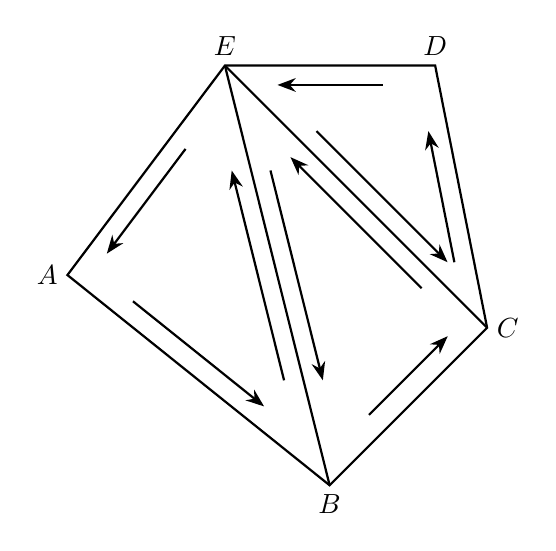
\begin{tikzpicture}
            \coordinate (A) at (0, 2.67);
            \coordinate (B) at (3.33, 0);
            \coordinate (C) at (5.33, 2);
            \coordinate (D) at (4.67, 5.33);
            \coordinate (E) at (2, 5.33);
            \draw[thick] (A) -- (B) -- (C) -- (D) -- (E) -- cycle;
            \draw[thick] (B) -- (E);
            \draw[thick] (C) -- (E);
            \halfarrow{[xshift=-7pt]B}{[xshift=-7pt]E}
            \halfarrow{[xshift=7pt]E}{[xshift=7pt]B}
            \halfarrow{[yshift=-11.2pt]E}{[yshift=-11.2pt]A}
            \halfarrow{[yshift=11.2pt]B}{[yshift=11.2pt]C}
            \halfarrow{[yshift=9.5pt]A}{[yshift=9.5pt]B}
            \halfarrow{[yshift=-9.4pt]C}{[yshift=-9.4pt]E}
            \halfarrow{[xshift=9.4pt]E}{[xshift=9.4pt]C}
            \halfarrow{[yshift=-7pt]D}{[yshift=-7pt]E}
            \halfarrow{[xshift=-7.14pt]C}{[xshift=-7.14pt]D}

            \node[anchor=east] at (A) {\(A\)};
            \node[anchor=north] at (B) {\(B\)};
            \node[anchor=west] at (C) {\(C\)};
            \node[anchor=south] at (D) {\(D\)};
            \node[anchor=south] at (E) {\(E\)};
        \end{tikzpicture}
        \caption{A closed polygonal chain internally triangulated, with orientations marked.}
        \label{fig:cauchyintegraltheoremoversimplyconnectedset_closedpolygonalchaintriangulation}
    \end{figure}Since \(P\) is a closed polygonal chain, we can triangulate the interior. For example, consider \autoref{fig:cauchyintegraltheoremoversimplyconnectedset_closedpolygonalchaintriangulation}. Then, \begin{align*}
        \int_{ABCDE}f(z)\ddz & =\qty(\int_{\overrightarrow{AB}}+\int_{\overrightarrow{BC}}+\int_{\overrightarrow{CD}}+\int_{\overrightarrow{DE}}+\int_{\overrightarrow{EA}})f(z)\ddz \\
                             & \quad+\qty(\int_{\overrightarrow{BE}}+\int_{\overrightarrow{EB}}+\int_{\overrightarrow{CE}}+\int_{\overrightarrow{EC}})f(z)\ddz                       \\
                             & =\int_{\Delta{ABE}}f(z)\ddz+\int_{\Delta{BCE}}f(z)\ddz+\int_{\Delta{CDE}}f(z)\ddz.
    \end{align*} Thus, if the integral over every triangle in \(U\) vanishes, then \eqref{eq:cauchyintegraltheoremoversimplyconnectedset_statement} follows. Consider a triangle in \(U\) with boundary \(\Delta\). \begin{figure}
        \centering
        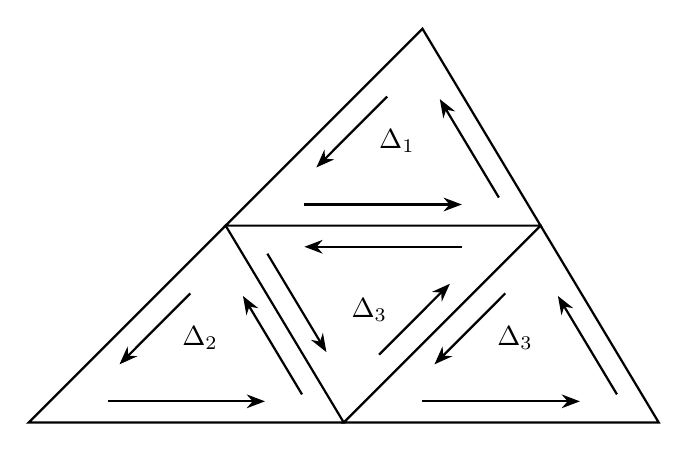
\begin{tikzpicture}
            \coordinate (A) at (0, 0);
            \coordinate (D) at (6.5, 2.5);
            \coordinate (F) at (2.5, 2.5);
            \coordinate (C) at (8, 0);
            \coordinate (B) at (5, 5);
            \coordinate (E) at (4, 0);

            \draw[thick] (A) -- (F) -- (E) -- cycle;
            \draw[thick] (B) -- (D) -- (F) -- cycle;
            \draw[thick] (C) -- (D) -- (E) -- cycle;

            \halfarrow{[yshift=-11.7pt]F}{[shift={(20pt, 8.2pt)}]A};
            \halfarrow{[yshift=-11.7pt]B}{[shift={(20pt, 8.2pt)}]F};
            \halfarrow{[yshift=-11.7pt]D}{[shift={(20pt, 8.2pt)}]E};
            \halfarrow{[yshift=11.7pt]E}{[shift={(-20pt, -8.2pt)}]D};

            \halfarrow{[shift={(-4.41pt, -7.64pt)}]E}{[shift={(-4.41pt, -7.64pt)}]F};
            \halfarrow{[shift={(-4.41pt, -7.64pt)}]D}{[shift={(-4.41pt, -7.64pt)}]B};
            \halfarrow{[shift={(-4.41pt, -7.64pt)}]C}{[shift={(-4.41pt, -7.64pt)}]D};
            \halfarrow{[shift={(4.41pt, 7.64pt)}]F}{[shift={(4.41pt, 7.64pt)}]E};

            \halfarrow{[yshift=7.64pt]A}{[yshift=7.64pt]E};
            \halfarrow{[yshift=7.64pt]E}{[yshift=7.64pt]C};
            \halfarrow{[yshift=7.64pt]F}{[yshift=7.64pt]D};
            \halfarrow{[yshift=-7.64pt]D}{[yshift=-7.64pt]F};

            \coordinate (AE) at ($(A)!0.5!(E)$);
            \coordinate (AF) at ($(A)!0.5!(F)$);
            \coordinate (FD) at ($(F)!0.5!(D)$);
            \coordinate (BF) at ($(B)!0.5!(F)$);
            \coordinate (EC) at ($(E)!0.5!(C)$);

            \path let
            \p1 = (FD),
            \p2 = (BF),
            \p3 = (AE),
            \p4 = (AF),
            \p5 = (EC)
            in
            node[shift={(5pt,-5pt)}] at (\x1, \y2) {\(\Delta_1\)}
            node[shift={(5pt,-5pt)}] at (\x3, \y4) {\(\Delta_2\)}
            node[shift={(5pt,-5pt)}] at (\x5, \y4) {\(\Delta_3\)}
            node[shift={(-5pt, 5pt)}] at (\x1, \y4) {\(\Delta_3\)};
        \end{tikzpicture}
        \caption{Quadrisection of the triangle bounded by \(\Delta\).}
        \label{fig:cauchyintegraltheoremoversimplyconnectedset_trianglequadrisection}
    \end{figure} Then define \(M\) to be \[M=\abs{\int_{\Delta}f(z)\ddz}.\]
    We can quadrisect the triangle bounded by \(\Delta\) into four triangles with boundaries \(\Delta_1,\Delta_2,\Delta_3,\Delta_4\) as in \autoref{fig:cauchyintegraltheoremoversimplyconnectedset_trianglequadrisection}. Then one of \(\Delta_1\), \(\Delta_2\), \(\Delta_3,\), and \(\Delta_4\) (denote this to be \(\Delta^1\)) satisfy
    \[\abs{\int_{\Delta^1}f(z)\ddz}\geq\frac{M}{4},\]
    and recursively, choose \begin{equation}
        \abs{\int_{\Delta^2}f(z)\ddz}\geq\frac{M}{4^2},\ldots,\abs{\int_{\Delta^n}f(z)\ddz}\geq\frac{M}{4^n}. \label{eq:cauchyintegraltheoremoversimplyconnectedset_trianglelowerbound}
    \end{equation}
    Let \(L\) denote the perimeter of \(\Delta\). Then, the perimeters of \(\Delta^1, \Delta^2,\ldots\) respectively are \(\frac{L}{2},\frac{L}{2^2},\ldots\). As \(n\to\infty\), \(\Delta_n\) shrinks to a single point \(z_0\). Then, \(\forall n\in\mathbb{N}\), \(z_0\in\Delta^n\).

    By the definition of holomorphy, \(\forall\varepsilon>0\), \(\exists\delta>0\) such that \(\forall z\in D\paren{z_0,\delta}\), \[\abs{\frac{f\paren{z}-f\paren{z_0}}{z-z_0}-f'\paren{z_0}}<\varepsilon,\]\[\abs{f\paren{z}-f\paren{z_0}-f'\paren{z_0}\paren{z-z_0}}<\varepsilon\abs{z-z_0}.\] and \(\exists N\in\mathbb{N}\) such that \(\forall n\in \mathbb{N}_{>N}\), \(\Delta^n\subset D\paren{z_0,\delta}\). By \autoref{thm:cauchyintegraltheorem}, since the functions \(1\) and \(z\) are both entire, \[\int_{\Delta^n}\ddz=0,\quad\int_{\Delta^n}z\ddz=0.\] Then
    \begin{align*}
        \int_{\Delta^n}f(z)\ddz & =\int_{\Delta^n}f(z)\ddz-f\paren{z_0}\int_{\Delta^n}\ddz-f'\paren{z_0}\left(\int_{\Delta^n}z\ddz-z_0\int_{\Delta^n}\ddz\right) \\
                                & =\int_{\Delta^n}\brackets{f(z)-f\paren{z_0}-f'\paren{z_0}\paren{z-z_0}}\ddz.
    \end{align*}
    Because the distance between any two points in the interior of a triangle is always less than its perimeter, using the triangle inequality for complex integrals, \[\int_{\Delta^n}\abs{f(z)}\abs{\ddz}\leq\varepsilon\int_{\Delta^n}\abs{z-z_0}\abs{\ddz}=\frac{\varepsilon L}{2^n}\int_{\Delta^n}\abs{\ddz}=\frac{\varepsilon L^2}{4^n}.\]
    Comparing the above equation with equation~\eqref{eq:cauchyintegraltheoremoversimplyconnectedset_trianglelowerbound}, \[\frac{M}{4^n}<\frac{\varepsilon L}{4^n},\quad M<\varepsilon L.\] Since \(\Delta\) is rectifiable, \(L\) is finite, and letting \(\varepsilon\to0\), we find that \(M\to0\). Then, for every triangle in \(U\), the integral vanishes, and equations \eqref{eq:cauchyintegraltheoremoversimplyconnectedset_chainvanishingstatement} and \eqref{eq:cauchyintegraltheoremoversimplyconnectedset_chaindefinition} follow.
\end{proof}
\begin{theorem}[Cauchy--Goursat Integral Theorem]\label{thm:cauchygoursattheorem}
    Let \(U\subset\mathbb{C}\) be an open region bounded with boundary \(\partial U\). Let \(f:U\to\mathbb{C}\) be a holomorphic function continuous on \(\overline{U}\). Then, \[\oint_{\partial U}f(\zeta)\ddzeta=0.\]
\end{theorem}
\begin{proof}
    Since \(\partial U\cap U=\emptyset\) and \(f(z)\) is not necessarily holomorphic over \(\overline{U}\), we cannot directly apply \autoref{lemma:cauchyintegraltheoremoversimplyconnectedset}.
    \begin{figure}
        \centering
        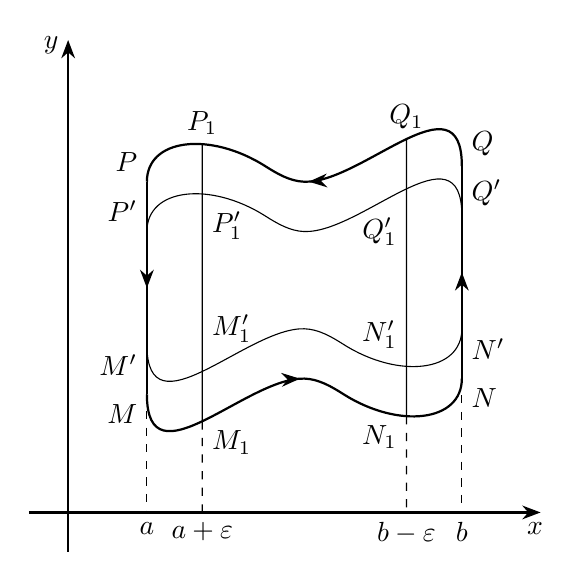
\begin{tikzpicture}[>=stealth,
                arrow style/.style={
                        postaction={decorate},
                        decoration={markings, mark=at position 0.5 with {\arrow[scale=1]{Stealth}}}
                    }]
            \pgfmathsetmacro{\lengtheta}{18pt}
            \pgfmathsetmacro{\lengthepsilon}{20pt}
            \coordinate (M) at (1, 1.5);
            \coordinate (P) at (1, 4.2);
            \coordinate (Q) at (5, 4.4);
            \coordinate (N) at (5, 1.7);
            \coordinate (Mprime) at ([yshift=\lengtheta] M);
            \coordinate (Pprime) at ([yshift=-\lengtheta] P);
            \coordinate (Qprime) at ([yshift=-\lengtheta] Q);
            \coordinate (Nprime) at ([yshift=\lengtheta] N);
            \draw[-{Stealth}, thick] (-0.5, 0) -- (6, 0);
            \draw[-{Stealth}, thick] (0, -0.5) -- (0, 6);
            \draw[thick, arrow style] (P) -- (M);
            \draw[thick, arrow style, name path=curveQP] (Q) to[out angle=90, in angle=90, curve through = {([shift={(2, 0)}] P) ([shift={(1.5, 0.2)}] P)}] (P);
            \draw[thick, arrow style] (N) -- (Q);
            \draw[thick, arrow style, name path=curveMN] (M) to[out angle=270, in angle=270, curve through = {([shift={(-2, 0)}] N) ([shift={(-1.5, -0.2)}] N)}] (N);
            \path let \p1 = (P) in coordinate (P1x) at ({\x1 + \lengthepsilon}, 0);
            \path let \p1 = (Q) in coordinate (Q1x) at ({\x1 - \lengthepsilon}, 0);
            \path[name path=verticalleftmarker](P1x) -- (P1x |- 0, 6);
            \path[name path=verticalrightmarker](Q1x) -- (Q1x |- 0, 6);
            \path[name intersections={of=curveQP and verticalleftmarker, by=P1}];
            \path[name intersections={of=curveMN and verticalleftmarker, by=M1}];
            \draw[thin] (M1) -- (P1);
            \path[name intersections={of=curveQP and verticalrightmarker, by=Q1}];
            \path[name intersections={of=curveMN and verticalrightmarker, by=N1}];
            \draw[thin] (N1) -- (Q1);
            \draw[thin] (Mprime) to[out angle=270, in angle=270, curve through = {([shift={(-2, 0)}] Nprime) ([shift={(-1.5, -0.2)}] Nprime)}] (Nprime);
            \draw[thin] (Qprime) to[out angle=90, in angle=90, curve through = {([shift={(2, 0)}] Pprime) ([shift={(1.5, 0.2)}] Pprime)}] (Pprime);
            \draw[dashed] (M) -- (M |- 0, 0);
            \draw[dashed] (N) -- (N |- 0, 0);
            \draw[dashed] (M1) -- (P1x);
            \draw[dashed] (N1) -- (Q1x);
            \node[anchor=north east] at (M) {\(M\)};
            \node[anchor=south east] at (P) {\(P\)};
            \node[anchor=south west] at (Q) {\(Q\)};
            \node[anchor=north west] at (N) {\(N\)};
            \node[anchor=north east] at (Mprime) {\(M'\)};
            \node[anchor=south east] at (Pprime) {\(P'\)};
            \node[anchor=south west] at (Qprime) {\(Q'\)};
            \node[anchor=north west] at (Nprime) {\(N'\)};
            \node[anchor=north west] at (M1) {\(M_1\)};
            \node[anchor=south] at (P1) {\(P_1\)};
            \node[anchor=south] at (Q1) {\(Q_1\)};
            \node[anchor=north east] at (N1) {\(N_1\)};
            \node[anchor=south west] at ([yshift=\lengtheta+7pt] M1) {\(M'_1\)};
            \node[anchor=north west] at ([yshift=-\lengtheta-3pt] P1) {\(P'_1\)};
            \node[anchor=north east] at ([yshift=-\lengtheta-7pt] Q1) {\(Q'_1\)};
            \node[anchor=south east] at ([yshift=\lengtheta+3pt] N1) {\(N'_1\)};
            \node[anchor=north] at (M |- 0, 0) {\(a\)};
            \node[anchor=north] at (N |- 0, 0) {\(b\)};
            \node[anchor=north] at (P1x |- 0, 0) {\(a+\varepsilon\)};
            \node[anchor=north] at (Q1x |- 0, 0) {\(b-\varepsilon\)};
            \node[anchor=north, xshift=-2pt] at (6, 0) {\(x\)};
            \node[anchor=east, yshift=-2pt] at (0, 6) {\(y\)};
        \end{tikzpicture}
        \caption{A simplified region containing two vertical lines and two continuous, rectifiable curves.}
        \label{fig:cauchygoursattheorem_simplifiedregion}
    \end{figure}

    First assume \(U\) has the shape of \(MNQP\) in \autoref{fig:cauchygoursattheorem_simplifiedregion}. That is, \(U\) consists of \(x=a\), \(x=b\) for \(a<b\), and two rectifiable \(C^0\) curves \(\overrightarrow{MN}:y=\varphi(x)\) and \(\overrightarrow{QP}:\psi(x)\) such that \(\varphi(x)<\psi(x)\), \(\forall a\le x\le b\).

    For some \(\varepsilon>0\), \(\eta>0\), construct a new curve \(M_1'N_1'Q_1'P_1'\in U\) to be the boundary of the region bounded by \(P_1M_1:x=a+\varepsilon\), \(N_1Q_1:b-\varepsilon\), \(M'N':\varphi(x)+\eta\), and \(Q'P': \psi(x)-\eta\) such that \(M_1'N_1'Q_1'P_1'\) remains simple. By \autoref{lemma:cauchyintegraltheoremoversimplyconnectedset}, \[\oint_{M_1'N_1'Q_1'P_1'}f(z)\ddz=0.\]
    By \autoref{lemma:uniformcontinuousovercompactset}, \(f(z)\) is uniformly continuous over \(\overline{U}\), and therefore \(\forall\varepsilon'>0\), we can choose \(\eta>0\) so that \(\forall z\in\overrightarrow{M_1'N_1'}\), \(\abs{f\paren{z}-f\paren{z-\eta}}<\varepsilon'\) is satisfied. Letting \(\eta\to0\) (with \(\varepsilon'\to0\)) and fixing \(\varepsilon>0\), we get that
    \begin{align*}
        \abs{\int_{\overrightarrow{M_1'N_1'}}f(z)\ddz-\int_{\overrightarrow{M_1N_1}}f(z)\ddz} & \leq\int_{\overrightarrow{M_1'N_1'}}\abs{f(z)-f\paren{z-\eta}}\abs{\ddz} \\
                                                                                              & <\varepsilon'\int_{\overrightarrow{M_1'N_1'}}\abs{dz}\to0,
    \end{align*}
    and consequently, \begin{equation}
        \int_{\overrightarrow{M_1'N_1'}}f(z)\ddz\to \int_{\overrightarrow{M_1N_1}}f(z)\ddz.\label{eq:cauchygoursattheorem_innerinnerhorizontaltoouterinnerhorizontal1}
    \end{equation}
    Under the same limit, we get \begin{equation}
        \int_{\overrightarrow{Q_1'P_1'}}f(z)\ddz\to \int_{\overrightarrow{Q_1P_1}}f(z)\ddz.\label{eq:cauchygoursattheorem_innerinnerhorizontaltoouterinnerhorizontal2}
    \end{equation} By the continuity of \(f(z)\) over a compact set, \begin{equation}
        \int_{\overrightarrow{P_1'M_1'}}f(z)\ddz\to \int_{\overrightarrow{P_1M_1}}f(z)\ddz,\quad\int_{\overrightarrow{N_1'Q_1'}}f(z)\ddz\to \int_{\overrightarrow{N_1Q_1}}f(z)\ddz.\label{eq:cauchygoursattheorem_innerinnerverticaltoouterinnervertical}
    \end{equation}
    Then letting \(\varepsilon\to0\), for the same reason as equation~\eqref{eq:cauchygoursattheorem_innerinnerverticaltoouterinnervertical}, equations \eqref{eq:cauchygoursattheorem_innerinnerhorizontaltoouterinnerhorizontal1} and \eqref{eq:cauchygoursattheorem_innerinnerhorizontaltoouterinnerhorizontal2} yield \[\int_{\overrightarrow{M_1N_1}}f(z)\ddz\to \int_{\overrightarrow{MN}}f(z)\ddz,\quad\int_{\overrightarrow{Q_1P_1}}f(z)\ddz\to \int_{\overrightarrow{QP}}f(z)\ddz.\]
    We are left to show the subsequent limits of the results from equation~\eqref{eq:cauchygoursattheorem_innerinnerverticaltoouterinnervertical}. For the left integral, let \(y_{\varphi}=\max\paren{\varphi(a),\varphi\paren{a+\varepsilon}}\) and \(y_{\psi}=\max\paren{\psi(a),\psi\paren{a+\varepsilon}}\).

    Then, \[\int_{\overrightarrow{PM}}f(z)\ddz=i\int_{\psi(a)}^{\varphi(a)}f\paren{a+iy}\ddy=i\paren{\int_{\psi(a)}^{y_\varphi}+\int_{y_\varphi}^{y_\psi}+\int_{y_\psi}^{\varphi(a)}}f(a+iy)\ddy.\]
    Similarly, \[\int_{\overrightarrow{P_1M_1}}f(z)\ddz=i\paren{\int_{\psi(a+\varepsilon)}^{y_\varphi}+\int_{y_\varphi}^{y_\psi}+\int_{y_\psi}^{\varphi(a+\varepsilon)}}f(a+\varepsilon+iy)\ddy.\]
    The difference \(\paren{\int_{\overrightarrow{PM}}-\int_{\overrightarrow{P_1M_1}}}f(z)\ddz\) between the two is then equal to \begin{gather*}
        i\int_{y_{\varphi}}^{y_{\psi}}\paren{f\paren{a+iy}-f\paren{a+\varepsilon+iy}}\ddz\\
        {}+{i\paren{\int_{\psi(a)}^{y_\varphi}+\int_{y_\psi}^{\varphi(a)}}f(a+iy)-i\paren{\int_{\psi(a+\varepsilon)}^{y_\varphi}z+\int_{y_\psi}^{\varphi\paren{a+\varepsilon}}}f(a+\varepsilon+iy)}.
    \end{gather*}
    The first term vanishes by uniform continuity (through the same argument used for \(M_1'N_1'\to M_1N_1\)) and the remaining four integrals all equal 0 as they are all integrable on a degenerating interval (as \(\varepsilon\to0\), \(y_\varphi\to\varphi(a)\) and \(y_\psi\to\psi(a)\) because \(\varphi, \psi\in C^0\)). Therefore, \[\int_{\overrightarrow{P_1M_1}}f(z)\ddz\to\int_{\overrightarrow{PM}}f(z)\ddz,\]
    and through similar logic, \[\int_{\overrightarrow{N_1Q_1}}f(z)\ddz\to\int_{\overrightarrow{NQ}}f(z)\ddz.\] Therefore, \[\oint_{MNQP}f(z)\ddz=0.\]
    Any open region \(U\subset\mathbb{C}\) with a simple closed boundary can be broken up into smaller regions with the same form as \(MNQP\) with finitely many auxiliary lines. Then the conclusion follows.
\end{proof}
\begin{remark}
    The theorem is also valid for any multiply connected region (and its boundary will consist of multiple curves) as a multiply connected region is equal to the union of several simply connected regions with vertical auxiliary lines between.

    Additionally, if \(U\subset\mathbb{C}\) is simply connected and \(f\) is holomorphic on \(U\), then for any two points \(z,z_0\in U\), the integral \[\int_{z_0}^zf(\zeta)\ddzeta\] is well-defined and independent of the path taken from \(z_0\) to \(z\). In this sense, a holomorphic function behaves analogously to a potential field.
\end{remark}
\begin{theorem}[Cauchy--Goursat Integral Formula]\label{thm:cauchygoursatformula}
    Let \(U\subset\mathbb{C}\) be an open region bounded with a simple closed boundary \(\partial U \), and let \(f:U\to\mathbb{C}\) be a holomorphic function continuous on \(\overline{U}\). Then for all \(z\in U\),
    \begin{equation}
        f(z)=\frac{1}{2\pi i}\oint_{\partial U}\frac{f(\zeta)}{\zeta-z}\ddzeta.\label{eq:cauchygoursatformula}
    \end{equation}
\end{theorem}
\begin{proof}
    By the Cauchy--Goursat Integral Theorem (\autoref{thm:cauchygoursattheorem}), \[\int_{\partial\paren{U\setminus D(z,\varepsilon)}}\frac{f(\zeta)}{\zeta-z}\ddzeta=\oint_{\partial U}\frac{f(\zeta)}{\zeta-z}\ddzeta-\oint_{\partial D(z,\varepsilon)}\frac{f(\zeta)}{\zeta-z}\ddzeta=0.\]
    From rearrangement, \[\oint_{\partial U}\frac{f(\zeta)}{\zeta-z}\ddzeta=2\pi if(z)+i\int_0^{2\pi}\paren{f\paren{z+\varepsilon e^{it}}-f(z)}\dd{t}.\]
    Since \(f\in C^0(\partial D(z,\varepsilon))\), as \(\varepsilon\to0\), \begin{align*}
        \abs{\int_0^{2\pi}\paren{f\paren{z+\varepsilon e^{it}}-f(z)}\dd{t}} & \leq\int_0^{2\pi}\abs{f\paren{z+\varepsilon e^{it}}-f(z)}\dd{t} \\
                                                                            & \leq2\pi\max\abs{f\paren{z+\varepsilon e^{it}}-f(z)}\to0.
    \end{align*}
    By rearrangement, \[f(z)=\frac{1}{2\pi i}\oint_{\partial U}\frac{f(\zeta)}{\zeta-z}\ddzeta.\]
\end{proof}
\begin{remark}
    In the proof of \autoref{thm:pompeiu}, we used Lipschitz continuity for a smooth function, which was a stronger condition than necessary. The true necessity of smoothness was to be able to apply Green's Theorem (\autoref{thm:complexgreen}).
\end{remark}
This profound theorem is extremely important and helpful in complex integration and essential in the evaluation of integrals, as demonstrated below.
\begin{example}\label{ex:cauchygoursatformularootsofunity}
    Evaluate the integral \(\int_{\partial D(0,2)}\frac{\ddz}{z^n-1}\), where \(n\in\mathbb{N}_{\geq 2}\).
\end{example}
\begin{proof}
    Since \(z^n-1=\prod_{k=0}^{n-1}\qty(z-\omega^k_n)\), where \(\omega^k_n=e^{i\pi\frac{k}{n}}\), the integrand has singularities at every \(n\)th root of unity. Then the integral is equal to: \begin{equation}
        \int_{\partial D(0,2)}\frac{\ddz}{\prod_{j=0}^{n-1}\qty(z-\omega_j)}=\int_{\partial D(0,2)}\sum_{j=0}^{n-1}\frac{c_j}{z-\omega_j}\ddz,\label{eq:cauchygoursatformularootsofunity}
    \end{equation}
    where \(\cbraces{c_j}\) are the coefficients of the partial fraction decomposition. By the Cauchy--Goursat Integral Formula (\autoref{thm:cauchygoursatformula}), equation~\eqref{eq:cauchygoursatformularootsofunity} becomes: \[\sum_{k=0}^{n-1}\int_{\partial D(0,2)}\frac{c_k}{z-\omega_k}\ddz=2\pi i\sum_{k=0}^{n-1}c_k.\]
    Observe that \(\sum_{k=0}^{n-1} c_k=\lim_{z\to\infty}\sum_{k=0}^{n-1}\frac{zc_k}{z-\omega_k}=\lim_{z\to\infty}\frac{z}{z^n-1}=0\) since \(n\geq2\).
    Therefore, \[\int_{\partial D(0,2)}\frac{\ddz}{z^n-1}=0.\]
\end{proof}
We have also already seen the utility of parameterization via a polar transformation. Many useful identities in classical calculus can also be derived from concepts in its generalization:
\begin{example}
    Prove that \(\forall n\in\mathbb{N}\), \[\int_{0}^{2\pi}\cos^{2n}\theta\dd{\theta}=2\pi\prod_{k=1}^n\frac{2k-1}{2k}.\]
\end{example}
\begin{proof}
    Consider the integral \[\int_{\partial\mathbb{D}}\qty(z+\frac{1}{z})^{2n}\frac{\ddz}{z}.\]
    Letting \(z=e^{i\theta}\), we get \(\int_{\partial\mathbb{D}}\qty(e^{i\theta}+e^{-i\theta})^{2n}e^{-i\theta}\ddz=2^{2n}i\int_0^{2\pi}\cos^{2n}\theta\dd{\theta}\). Alternatively, we can expand the integrand and get \[\int_{\partial\mathbb{D}}\sum_{k=0}^{2n}\binom{2n}{k}z^{2k-2n}\frac{\ddz}{z}=\sum_{k=0}^{2n}\int_{\partial\mathbb{D}}\binom{2n}{k}z^{2k-2n-1}\ddz.\]
    When \(2k-2n-1\ge0\), the integrand is holomorphic. The integral is then equal to \[\binom{2n}{0}\int_{\partial\mathbb{D}}z^{-2n-1}\ddz+\binom{2n}{1}\int_{\partial\mathbb{D}}z^{-2n+1}\ddz+\cdots+\binom{2n}{n}\int_{\partial\mathbb{D}}\frac{\ddz}{z}=2\pi i\binom{2n}{n},\]
    since all of the higher order terms vanish:
    \[\int_{\partial\mathbb{D}}z^{2k-2n-1}\ddz=\int_0^{2\pi} e^{i\theta\qty(2k-2n-1)}ie^{i\theta}\dd{\theta}=i\int_0^{2\pi}e^{2i\theta(k-n)}\dd{\theta}=\begin{cases}
            0      & k< n \\
            2\pi i & k=n
        \end{cases}.\]
    Therefore, \[2^{2n}i\int_0^{2\pi}\cos^{2n}\theta\dd{\theta}=2\pi i\binom{2n}{n}\Longleftrightarrow\int_0^{2\pi}\cos^{2n}\theta\dd{\theta}=2\pi\frac{\qty(2n)!}{2^{2n}\qty(n!)^2}=2\pi\frac{\prod_{k=1}^{2n}k}{\qty[\prod_{k=1}^{n}\qty(2k)]^2}.\]
    From simple cancellation, we get \[2\pi\frac{\prod_{k=1}^{n}\qty(2k-1)}{\prod_{k=1}^n\qty(2k)}=2\pi\prod_{k=1}^n\frac{2k-1}{2k},\]
    as expected.
\end{proof}
\subsection{Analyticity and Holomorphy}\label{sec:analyticityandholomorphy}
The Cauchy--Goursat Integral Formula (\autoref{thm:cauchygoursatformula}) can also be generalized into a result that equates complex integration and differentiation:
\begin{theorem}[Cauchy--Goursat Differentiation Formula]\label{thm:cauchydifferentiationformula}
    Let \(U\subset\mathbb{C}\) be an open region bounded by a simple closed boundary \(\partial U\), and let \(f:U\to\mathbb{C}\) be holomorphic and continuous over \(\overline{U}\). Then \(\forall z\in U\), \(\forall n\in\mathbb{N}\), \(f^{(n)}(z)\) exists, and
    \begin{equation}
        f^{(n)}(z)=\frac{n!}{2\pi i}\oint_{\partial U}\frac{f(\zeta)}{\paren{\zeta-z}^{n+1}}\ddzeta.\label{eq:cauchydifferentiationformula_statement}
    \end{equation}
    Additionally, by the openness of \(U\), \(\forall z_0\in U\), \(\exists r>0\) such that the closed disk \(\overline{D\paren{z_0,r}}\subset U\) and that \(\forall z\in\overline{D\paren{z_0,r}}\), \(f(z)\) has the uniformly and absolutely convergent Taylor expansion
    \begin{equation}
        f(z)=\sum_{j=0}^\infty a_j\paren{z-z_0}^j,\label{eq:cauchydifferentiationformula_taylorseries}
    \end{equation}
    where \begin{equation}
        a_j=\frac{1}{2\pi i}\oint_{\partial U}\frac{f(\zeta)}{\paren{\zeta-z}^{j+1}}\ddzeta.\label{eq:cauchydifferentiationformula_taylorseriescoefficients}
    \end{equation}
\end{theorem}
\begin{proof}
    \(\forall z_0\in U\), \(\forall z\in D\paren{z_0,r}\subset U\), by \autoref{thm:cauchygoursatformula}, \[f(z)-f\paren{z_0}=\frac{1}{2\pi i}\oint_{\partial U}\paren{\frac{f(\zeta)}{\zeta-z}-\frac{f(\zeta)}{\zeta-z_0}}\ddzeta=\frac{z-z_0}{2\pi i}\oint_{\partial U}\frac{f(\zeta)\ddzeta}{\paren{\zeta-z}\paren{\zeta-z_0}},\]
    and dividing by \(z-z_0\), the above is equal to \[\frac{f(z)-f\paren{z_0}}{z-z_0}=\frac{1}{2\pi i}\oint_{\partial U}\frac{f(\zeta)\ddzeta}{\paren{\zeta-z}\paren{\zeta-z_0}}.\]
    Since \begin{align}
        \frac{f(z)-f\paren{z_0}}{z-z_0}-\frac{1}{2\pi i}\oint_{\partial U}\frac{f(\zeta)\ddzeta}{\paren{\zeta-z_0}^2} & =\frac{1}{2\pi i}\oint_{\partial U}\frac{f\paren{\zeta}}{\zeta-z_0}\paren{\frac{1}{\zeta-z}-\frac{1}{\zeta-z_0}}\ddzeta\nonumber                                      \\
                                                                                                                      & =\frac{z-z_0}{2\pi i}\oint_{\partial U}\frac{f(\zeta)}{(\zeta-z)\paren{\zeta-z_0}^2}\ddzeta.\label{eq:cauchydifferentiationformula_differenceoffirstorderdifferences}
    \end{align}
    Let \(d\) be the distance from \(z_0\) to \(\partial U\), and choose \(r=\frac{d}{2}\). Then, since \(\abs{z-z_0}<\frac{d}{2}\) and \(\abs{\zeta-z_0}\geq d\), \(\abs{\zeta-z}\geq\frac{d}{2}\). Then the absolute value of the integrand of equation~\eqref{eq:cauchydifferentiationformula_differenceoffirstorderdifferences} is bounded above by \(\frac{2M}{d^3}\), where \(M\) is the maximum of \(f(\zeta)\), which exists by \autoref{thm:continuousfunctionboundedoncompact}. Then, \[\abs{\frac{z-z_0}{2\pi i}\oint_{\partial U}\frac{f(\zeta)}{(\zeta-z)\paren{\zeta-z_0}^2}\ddzeta}\leq\frac{\abs{z-z_0}}{\pi}\frac{M}{d^3}\oint_{\partial U}\abs{\ddzeta}.\] As \(z\to z_0\), the difference vanishes, and therefore, \[f'\paren{z_0}=\frac{1}{2\pi i}\oint_{\partial U}\frac{f(\zeta)}{\paren{\zeta-z_0}^2}\ddzeta.\]
    Now inductively assume that equation~\eqref{eq:cauchydifferentiationformula_statement} is true for a given \(n=k\in\mathbb{N}\), or \[f^{(k)}(z)=\frac{k!}{2\pi i}\oint_{\partial U}\frac{f(\zeta)}{\paren{\zeta-z}^{k+1}}\ddzeta.\]
    Notice the expansion of the kernel, convergent since \(\abs{z-z_0}<\abs{\zeta-z_0}\):
    \begin{equation}
        \frac{1}{\zeta-z}=\frac{1}{\zeta-z_0}\cdot\frac{\zeta-z_0}{\zeta-z}=\frac{1}{\zeta-z_0}\cdot\frac{1}{1-\frac{z-z_0}{\zeta-z_0}}=\frac{1}{\zeta-z_0}\sum_{j=0}^{\infty}\paren{\frac{z-z_0}{\zeta-z_0}}^j.\label{eq:cauchydifferentiationformula_kernelexpansion}
    \end{equation}
    Then, \begin{align*}
        f^{(k)}(z) & =\frac{k!}{2\pi i}\oint_{\partial U}\frac{f(\zeta)}{(\zeta-z)^{k+1}}\ddzeta                                                                           \\
                   & =\frac{k!}{2\pi i}\oint_{\partial U}\frac{f(\zeta)}{\paren{\zeta-z_0}^{k+1}}\paren{\sum_{j=0}^{\infty}\paren{\frac{z-z_0}{\zeta-z_0}}^j}^{k+1}\ddzeta \\
                   & =f^{(k)}\paren{z_0}+\frac{(k+1)!\paren{z-z_0}}{2\pi i}\oint_{\partial U}\frac{f(\zeta)}{\paren{\zeta-z_0}^{k+2}}\ddzeta                               \\
                   & \quad+\mathcal{O}_{z\to z_0}\paren{\abs{z-z_0}^2},
    \end{align*}
    where the remainder terms \(\mathcal{O}_{z\to z_0}\qty(\abs{z-z_0}^2)\) resemble
    \[\paren{z-z_0}^2\frac{k!}{2\pi i}\brackets{k+1+\binom{k+1}{2}}\oint_{\partial U}\frac{f(\zeta)}{\paren{\zeta-z_0}^{k+3}}\ddzeta+\mathcal{O}_{z\to z_0}\paren{\abs{z-z_0}^3}.\]
    The difference quotient is equal to \[\frac{f^{(k)}(z)-f^{(k)}\paren{z_0}}{z-z_0}=\frac{(k+1)!}{2\pi i}\oint_{\partial U}\frac{f(\zeta)}{\paren{\zeta-z_0}^{k+2}}\ddzeta+\mathcal{O}_{z\to z_0}\abs{z-z_0}.\] As \(z\to z_0\), the remainder terms vanish, and \[f^{(k+1)}\paren{z_0}=\frac{(k+1)!}{2\pi i}\oint_{\partial U}\frac{f(\zeta)}{\paren{\zeta-z_0}^{k+2}}\ddzeta.\]
    By induction, equation~\eqref{eq:cauchydifferentiationformula_statement} is valid. By substituting equation~\eqref{eq:cauchydifferentiationformula_kernelexpansion} into \eqref{eq:cauchygoursatformula}, we obtain \[f(z)=\frac{1}{2\pi i}\oint_{\partial U}\frac{f(\zeta)}{\zeta-z_0}\sum_{j=0}^{\infty}\paren{\frac{z-z_0}{\zeta-z_0}}^j\ddzeta=\frac{1}{2\pi i}\oint_{\partial U}\sum_{j=0}^{\infty}\paren{z-z_0}^j\frac{f(\zeta)\ddzeta}{\paren{\zeta-z_0}^{j+1}}.\]
    Because \(f(\zeta)\) is continuous over \(\partial U\), it is bounded by a constant \(M\). Additionally, since \(\abs{z-z_0}<\abs{\zeta-z_0}\), the sum is termwise bounded by the convergent series \[\sum_{j=0}^\infty\frac{Mr^j}{\inf_{\xi\in\partial U}\abs{\xi-z_0}^{j+1}}.\]
    By the Weierstrass \(M\)--Test (\autoref{thm:weierstrassmtest}), the series uniformly converges, and we can justify \begin{gather*}
        \frac{1}{2\pi i}\oint_{\partial U}\sum_{j=0}^{\infty}\paren{z-z_0}^j\frac{f(\zeta)}{\paren{\zeta-z_0}^{j+1}}\ddzeta=\frac{1}{2\pi i}\sum_{j=0}^{\infty}\oint_{\partial U}\paren{z-z_0}^j\frac{f(\zeta)}{\paren{\zeta-z_0}^{j+1}}\ddzeta\\=\sum_{j=0}^\infty a_j\paren{z-z_0}^j,
    \end{gather*}
    which verifies equations \eqref{eq:cauchydifferentiationformula_taylorseries} and \eqref{eq:cauchydifferentiationformula_taylorseriescoefficients}.
\end{proof}
\begin{remark}
    By induction, we have shown that assuming the existence of the first order derivative of a holomorphic function \(f\), the \(n\)th order derivative of \(f\) exists \(\forall n\in\mathbb{N}\) and is holomorphic over the same region as \(f^{(n-1)}\). Furthermore, if \(f\) is holomorphic, then \(\forall z\in U\), there exists an open disk enclosing \(z\) such that \(f\) has a convergent Taylor series expansion. This property is known as \textit{analyticity}, and \autoref{thm:cauchydifferentiationformula} tells us that all holomorphic functions are analytic. Analytic functions can be expanded into power series, which are termwise differentiable, and therefore complex differentiable. Thus, analyticity and holomorphy are logically equivalent, which is a fundamental difference between real and complex functions.
\end{remark}
The differentiation formula above can be thought of as a generalization of \autoref{thm:cauchygoursatformula}, and provides similar utility in the evaluation of integrals:
\begin{example}\label{ex:legendrepolynomialintegralformula}
    A \textit{Legendre polynomial} is a polynomial in the form of \begin{equation}
        P_n(z)=\frac{1}{2^nn!}\dv[n]{z}(\qty(z^2-1)^n),\label{eq:legendrepolynomialintegralformula_rodriguesformula}
    \end{equation} which is a formula given by Olinde Rodrigues. Prove the integral form \[P_n(z)=\frac{1}{2\pi i}\oint_\gamma\frac{\qty(\zeta^2-1)^n}{2^n(\zeta-z)^{n+1}}\ddzeta,\] where \(\gamma\) is a simple closed curve enclosing \(z\).
\end{example}
\begin{proof}
    From the Cauchy--Goursat Differentiation Formula (\autoref{thm:cauchydifferentiationformula}) on equation~\eqref{eq:legendrepolynomialintegralformula_rodriguesformula}, we get that \[P_n(z)=\frac{1}{2^{n+1}\pi i}\int_{\gamma}\frac{\qty(\zeta^2-1)^n}{(\zeta-z)^{n+1}}\ddzeta,\] as desired.
\end{proof}
\begin{theorem}[Cauchy's Estimate]\label{thm:cauchysestimate}
    For a function \(f:U\to\mathbb{C}\) holomorphic over \(U\subseteq\mathbb{C}\) and \(\forall z_0\in U\) and \(\forall R>0\) such that \(\overline{D\paren{z_0,R}}\subseteq{U}\), \(\forall n\in\mathbb{N}\), \[\abs{f^{(n)}\paren{z_0}}\leq\frac{n!M}{R^n},\]
    where \[M=\max_{z\in\overline{D\paren{z_0,R}}}\abs{f(z)}.\]
\end{theorem}
\begin{proof}
    By the Cauchy--Goursat Differentiation Formula (\autoref{thm:cauchydifferentiationformula}), \(\forall n\in\mathbb{N}\), \[f^{(n)}\paren{z_0}=\frac{n!}{2\pi i}\oint_{\partial D\paren{z_0,R}}\frac{f(\zeta)}{\paren{\zeta-z_0}^{n+1}}\ddzeta.\]
    Because \(f(z)\) is continuous over the boundary \(\partial D\paren{z_0,R}\), it is bounded by \(M\). Thus,
    \[\abs{f^{(n)}\paren{z_0}}\leq\frac{n!}{2\pi}\int_0^{2\pi}\frac{M}{\paren{e^{i\theta}R}^{n+1}}e^{i\theta}R\dd{\theta}=\frac{n!M}{R^n},\] as desired.
\end{proof}
\autoref{thm:nthderivativeboundedl1norm} will profoundly generalize this statement significantly. The relationship between the derivatives of a holomorphic function and the function itself is an important property of holomorphic functions.
\begin{example}
    Let \(f\) be entire and \(\forall z\in\mathbb{C}\), \(|f(z)|\leq Me^{|z|}\). Prove that \(\forall n\in\mathbb{N}\), \(|f(0)|\leq M\) and \[\abs{f^{(n)}(0)}\leq Mn!\qty(\frac{e}{n})^n.\]
\end{example}
\begin{proof}
    \(|f(0)|\leq M\) is obviously true by letting \(z=0\). Then \(\forall R>0\), by Cauchy's Estimate (\autoref{thm:cauchysestimate}), \[\abs{f^{(n)}(0)}\leq Mn!\frac{e^{R}}{R^n}.\]
    By letting \(R=n\), the conclusion follows. In fact, this is the tightest possible inequality. Consider \(\varphi(R)=Mn!\frac{e^R}{R^n}\) to be a function of \(R\). It attains its minimum as its derivative vanishes:
    \[\varphi'(R)=Mn!\frac{e^RR^n-ne^RR^{n-1}}{R^{2n}}=0\Longleftrightarrow R^n=nR^{n-1}\Longleftrightarrow R=n.\] To confirm it as a minimum, we calculate the second order derivative:
    \[\varphi''(R)=Mn!e^R\qty(\frac{1}{R^n}-\frac{2n}{R^{n+1}}+\frac{n(n+1)}{R^{n+2}})\Longrightarrow\varphi''(n)=M(n-1)!\frac{e^n}{n^n},\]
    which is positive and convex.
\end{proof}
\begin{theorem}[Liouville's Theorem]\label{thm:liouville}
    Any bounded entire function is constant.
\end{theorem}
\begin{proof}
    Let \(f:\mathbb{C}\to\mathbb{C}\) be entire. Then, \(\forall z_0\in\mathbb{C}\), \(\forall R>0\), \(f\) is holomorphic over \(\overline{D\paren{z_0,R}}\). By \autoref{thm:cauchysestimate}, \[\abs{f'\paren{z_0}}\leq\frac{M}{R},\] where \(M=\sup_{z\in\mathbb{C}}\abs{f(z)}\). By letting \(r\to\infty\), \(f'\paren{z_0}\) where \(z_0\) is any arbitrary value in \(\mathbb{C}\). Therefore, \(f(z)\) is constant.
\end{proof}
\begin{theorem}[Morera's Theorem]\label{thm:morera}
    Let \(U\subseteq\mathbb{C}\) and \(f:U\to\mathbb{C}\) be continuous over \(U\). If for any rectifiable closed curve \(\gamma\subset U\), \[\oint_{\gamma}f(\zeta)\ddzeta=0,\] then \(f\) is holomorphic over \(U\).
\end{theorem}
\begin{proof}
    Since the integral vanishes on any closed curve \(\gamma\), \(\forall z_0,z\in U\), the integral is path independent with endpoints \(z_0\) and \(z\):
    \[F(z)=\int_{z_0}^zf(\zeta)\ddzeta.\]
    As \(f(z)\) is continuous over \(U\), \(F(z)\) is continuous over \(U\) as well. \(F(z)\) is holomorphic over \(U\) (complex differentiable with \(F'(z)=f(z)\)), and by \autoref{thm:cauchydifferentiationformula}, the derivative of \(F(z)\), \(f(z)\) is also holomorphic over \(U\).
\end{proof}
\begin{theorem}\label{thm:nthderivativeboundedl1norm}
    Let \(U\subseteq\mathbb{C}\) be open, let \(K\subset U\) be compact and \(V\supset K\) be open such that \(\overline{V}\subset U\) (\(V\) is a neighborhood of \(K\) that is relatively compact in \(U\)). Let \(f(z)\) be holomorphic in \(U\). Then there exists a sequence \(\cbraces{c_n}\subset\mathbb{R}\) dependent only on \(K\) and \(V\) (independent from \(f\) and \(z\)) such that \(\forall n\in\mathbb{N}\), \begin{equation}
        \sup_{z\in K}\abs{f^{(n)}(z)}\leq c_n\left\|f\right\|_{L^1(V)},\label{eq:nthderivativeboundedl1norm_statement}
    \end{equation}
    where \(\left\|f\right\|_{L^p(V)}\) denotes \[\paren{\int_V\abs{f(z)}^p\ddx\wedge\ddy}^{\flatfrac{1}{p}}.\]
\end{theorem}
\begin{proof}
    Let \(\varphi\in C^\infty\paren{\mathbb{C}}\)  satisfy \(\supp(\varphi)\subset V\) and be identically equal to 1 over some open neighborhood \(W\) of \(K\) relatively compact in \(V\). Since \(f\in C^\infty\paren{U}\), by the Cauchy--Pompeiu Theorem (\autoref{thm:pompeiu}) on \(f(z)\varphi(z)\in C^\infty\paren{\overline{U}}\), \[f(z)\varphi(z)=\frac{1}{2\pi i}\paren{\int_{\partial U}\frac{f(\zeta)\varphi(\zeta)}{\zeta-z}\ddzeta-\int_{U}\pdv{f(\zeta)\varphi(\zeta)}{\overline{\zeta}}\cdot\frac{\dd{\overline{\zeta}}\wedge\ddzeta}{\zeta-z}}.\]
    By the product rule, \[\pdv{f(\zeta)\varphi(\zeta)}{\overline{\zeta}}=\pdv{\varphi(\zeta)}{\overline{\zeta}}f(\zeta),\] and since \(\partial U\subset\mathbb{C}\setminus\supp(\varphi)\), the first term vanishes, resulting in \[f(z)\varphi(z)=-\frac{1}{2\pi i}\int_U\pdv{\varphi(\zeta)}{\overline{\zeta}}f(\zeta)\cdot\frac{\dd{\overline{\zeta}}\wedge\ddzeta}{\zeta-z}.\] Let \(K_1\) denote \(\supp\paren{\pdv{\varphi(\zeta)}{\overline{\zeta}}}\), and \(\forall z\in K\), \(\varphi(z)=1\). Therefore, \[f(z)=\frac{1}{2\pi i}\int_{K_1}f(\zeta)\cdot\pdv{\varphi(\zeta)}{\overline{\zeta}}\cdot\frac{\ddzeta\wedge\dd{\overline{\zeta}}}{\zeta-z}.\]
    We can differentiate within the integral as \(f(\zeta)\cdot\pdv{\varphi(\zeta)}{\overline{\zeta}}\) is \(C^\infty\) and bounded over \(K_1\), and thus the integrand is uniformly bounded by an integrable function independent of \(\zeta\):
    \[f^{(n)}(z)=\frac{n!}{2\pi i}\int_{K_1} f(\zeta)\cdot\pdv{\varphi(\zeta)}{\overline{\zeta}}\cdot\frac{\ddzeta\wedge\dd{\overline{\zeta}}}{\paren{\zeta-z}^{n+1}},\]
    and by the triangle inequality,
    \[\abs{f^{(n)}(z)}\leq\frac{n!}{2\pi}\int_{K_1} \abs{f(\zeta)}\abs{\pdv{\varphi(\zeta)}{\overline{\zeta}}}\frac{\abs{\ddzeta\wedge\dd{\overline{\zeta}}}}{\abs{\zeta-z}^{n+1}}.\]
    Notice that over \(W\), \(\varphi=1\), \(\varphi'=0\), and is disjoint from \(K_1\) (or that \(W\cap K_1=\emptyset\)). Then, the distance between \(W\) and \(K\) is positive and the two are disjoint. Therefore, \(\exists M>0\) such that
    \[\frac{1}{\abs{\zeta-z}}\leq M,\] and thus, \[\abs{\pdv{\varphi(\zeta)}{\overline{\zeta}}}\frac{1}{\abs{\zeta-z}^{n+1}}\] can be bounded by a sequence \(\cbraces{c'_n}\), independent of \(f\) and dependent only on \(n\) and the sets \(K\) and \(V\). Then, \[\abs{f^{(n)}(z)}\leq\frac{n!}{2\pi}\int_{K_1}c'_n\abs{f(\zeta)}{\abs{\ddzeta\wedge\dd{\overline{\zeta}}}}=\frac{n!}{\pi}\int_{K_1}c'_n\abs{f(\zeta)}{\abs{\ddx\wedge\ddy}}.\] Because \(K_1\) is compact, it has a finite area \(\mu\paren{K_1}\), and we can define a new sequence \(c_n=\frac{n!}{\pi}c'_n\mu\paren{K_1}\) to find that \[\abs{f^{(n)}(z)}\leq c_n\int_{K_1}\abs{f(\zeta)}{\abs{\ddx\wedge\ddy}}\leq c_n\int_{V}\abs{f(\zeta)}{\abs{\ddx\wedge\ddy}}.\]

    The problem now stands to prove that \(\varphi(z)\) exists in the first place, which is discussed later in \autoref{thm:bumpfunctionexistence}.
\end{proof}
\begin{corollary}\label{crl:nthderivativeboundedsupremum}
    Let \(U\subseteq\mathbb{C}\) be open, let \(K\subset U\) be compact and \(V\supset K\) be open such that \(\overline{V}\subset U\). For any holomorphic function \(f(z)\) in \(U\), there exist constants (independent of \(z\) and \(f\)) \(\cbraces{c_n}\) such that \[\sup_{z\in K}\abs{f^{(n)}(z)}\leq c_n\sup_{z\in V}\abs{f(z)}.\]
\end{corollary}
\begin{proof}
    Starting from equation~\eqref{eq:nthderivativeboundedl1norm_statement}, observe that \[c_n\left\|f\right\|_{L^1(V)}\leq c_n\mu(V)\sup_{z\in V}\abs{f(z)},\] and we can define a new set of constants equal to \(c_n\mu(V)\), which are still independent of \(z\).
\end{proof}
For the next theorem we will briefly introduce the concept of \textit{analytic continuation}.
\begin{definition}[Analytic Continuation]
    Let \(U\subseteq\mathbb{C}\) be a region, let \(f:U\to\mathbb{C}\) be holomorphic, and
    let \(V\subseteq\mathbb{C}\) be a region with \(U\subseteq V\). A function
    \(F:V\to\mathbb{C}\) is an \textit{analytic continuation} of \(f\) to \(V\) if:
    \begin{enumerate}
        \item \(F\) is holomorphic on \(V\), and
        \item \(F(z)=f(z)\) for all \(z\in U\).
    \end{enumerate}
\end{definition}
\begin{theorem}[Riemann's Theorem on Removable Singularities]\label{thm:removablesingularitiesriemann}
    Let \(D^*\qty(z_0,r)=D\paren{z_0,r}\setminus\cbraces{z_0}\), and \(f:D^*\paren{z_0,r}\to\mathbb{C}\) be holomorphic and bounded. Then \(f\) can be analytically continued to \(D\paren{z_0,r}\).
\end{theorem}
\begin{proof}
    Define the auxiliary function \[\varphi(z)=\begin{cases}
            \paren{z-z_0}^2f(z) & z\in D^*\paren{z_0,r} \\
            0                   & z=z_0
        \end{cases}.\]
    \(\varphi(z)\) is bounded and continuously differentiable on \(D\paren{z_0,r}\) and satisfies the Cauchy--Riemann Equations since
    \[\lim_{z\to z_0}\frac{\varphi(z)-\varphi\paren{z_0}}{z-z_0}=\frac{\paren{z-z_0}^2f(z)}{z-z_0}=\lim_{z\to z_0}\paren{z-z_0}f(z)=0,\] meaning that \(\dv{\varphi}{z}\paren{z_0}=0\). For \(z\in D^*\paren{z_0,r}\), \[\varphi'(z)=2\paren{z-z_0}f(z)+\paren{z-z_0}^2f'(z).\] As \(z\to z_0\), \(\varphi(z)\to0\), meaning that \(\varphi\) is holomorphic over \(D\paren{z_0,r}\). By \autoref{thm:cauchydifferentiationformula}, \[\varphi(z)=\sum_{j=2}^\infty a_j\paren{z-z_0}^j,\]
    which is convergent over \(D\paren{z_0,r}\). Then we can define \[\tilde{f}(z)=\frac{\varphi(z)}{\paren{z-z_0}^2}=\sum_{j=0}^\infty a_{j+2}\paren{z-z_0}^j\] over the same disk of convergence. Over the punctured disk, \(\tilde{f}(z)=f(z)\), and therefore \(\tilde{f}\) is an analytic continuation of \(f\).
\end{proof}
\subsubsection{Partitions of Unity and the Existence of Bump Functions}
\begin{definition}[Topological Space]
    A \textit{topological space} is a pair \((X, \tau)\), where \(X\) is a set and \(\tau\) is a collection of subsets of \(X\) satisfying the following properties:
    \begin{enumerate}
        \item \(\emptyset\in\tau\) and \(X\in\tau\),
        \item The union of any collection of sets in \(\tau\) is also in \(\tau\),
        \item The intersection of any finite number of sets in \(\tau\) is also in \(\tau\).
    \end{enumerate}
    The collection \(\tau\) is called a \textit{topology} on \(X\), and its elements are referred to as \textit{open sets} under the topology \(\tau\).
\end{definition}
If a topological space \(X\) can be written as the union between two nonempty disjoint open sets, then it is \textit{disconnected}. Otherwise, it is \textit{connected}.

A topology allows the definition and general conceptualization of continuity, convergence, and connectedness in a general setting, without necessarily relying on a notion of distance (a metric).

For example, in a topological space, a function \(f:X\to Y\) between two topological spaces is said to be continuous if the preimage of every open set in \(Y\) is an open set in \(X\). This generalizes the familiar \(\varepsilon\)-\(\delta\) definition of continuity from calculus.
\begin{example}
    To illustrate this, consider the function \(f:\mathbb{R} \to \mathbb{R}\) defined by
    \[f(x)=\begin{cases}
            1 & x\geq0, \\
            0 & x<0.\end{cases}
    \]
    We equip both the domain and codomain with the standard topology on \(\mathbb{R}\).
    Let us examine the open set \(V = (0.5, 1.5) \subseteq \mathbb{R}\). Then the preimage of \(V\) is \[f^{-1}(V) = \{x\in\mathbb{R}\mid f(x)\in(0.5,1.5)\}=[0, \infty),\]
    which is not an open set in the standard topology on \(\mathbb{R}\).
\end{example}
\begin{definition}[Basis of a Topology]
    For a topological space \((X,\tau)\), a \textit{basis} \(\mathcal{B}\subseteq\tau\) is a subcollection of \(\tau\) such that every set in \(\tau\) is equal to the union of a subcollection of \(\mathcal{B}\).
\end{definition}
It is easy to see that \(\mathcal{B}\) forms an open cover of \(X\). For any two sets in a topology, their intersection is also in the topology, which means there is a set in the basis of the topology that is a subset of the intersection.

In other words, \(\forall B_1,B_2\in\mathcal{B}\), \(\forall x\in B_1\cap B_2\), \(\exists B_3\in\mathcal{B}\) such that \(x\in B_3\) and \(B_3\subseteq B_1\cap B_2\).

In a topological space \(X\), a subset can either be open, closed (the complement of some open set), both (clopen), or neither.

Two clopen sets in any topological space \(X\) are \(\emptyset\) and \(X\). A technique used in many proofs in complex analysis follow from the following fact:
\begin{theorem}\label{thm:connectedtopologicalspaceclopensets}
    A topological space \(X\) is \textit{connected} if and only if \(X\) and \(\emptyset\) are the only clopen subsets of \(X\).
\end{theorem}
\begin{proof}
    Suppose that \(X\) is connected. Suppose that \(A\subseteq X\) is clopen. Notice that \(A\) and \(X\setminus A\) are both open in \(X\) by clopenness and are disjoint from each other. Since \(X=A\cup\qty(X\setminus A)\), it follows that either \(A=\emptyset\) or \(X\setminus A=\emptyset\Leftrightarrow A=X\).

    Conversely, for the sake of contradiction, assume \(X\) is disconnected. Then, there exist two nonempty open sets \(U,V\subseteq X\) such that \(U\cap V=\emptyset\) and \(U\cup V=X\). It follows that \(U=X\setminus V\neq X\) and \(V=X\setminus U\neq X\) are closed and consequently clopen. This contradicts the assumption that \(X\) and \(\emptyset\) are the only clopen subsets of \(X\).  Thus, \(X\) must be connected.
\end{proof}
\begin{example}
    The topological space \(\mathbb{R}\) under the standard topology only contains two clopen sets: \(\mathbb{R}\) and \(\emptyset\).

    The topological space of \(X=\paren{\bigcup_{n\in 2\mathbb{Z}}(n,n+1),\tau}\), where \(\tau\) is the unique topology formed by the basis \(\cbraces{(n,n+1)}{n\in 2\mathbb{Z}}\), which is disconnected. Consider \((0,1)\subset X\). Obviously, \((0,1)\in\tau\) so it is open. However, \(\bigcup_{n\in 2\mathbb{Z}}(n,n+1)\setminus (0,1)=\bigcup_{\substack{n\in 2\mathbb{Z}\\n\neq 0}}(n,n+1)\in\tau\), and therefore, \((0,1)\) is also closed under \(\tau\). In fact, every set in \(\tau\) is clopen.
\end{example}
\begin{definition}[Exhaustion by Compact Sets]\label{def:exhaustionbycompactsets}
    For a topological space \(X\), an \textit{exhaustion by compact sets} is a nested sequence of compact sets \(\cbraces{K_n}_{n\in\mathbb{N}}\subseteq X\), such that \(\forall n\in\mathbb{N}\), \(K_n\subset K_{n+1}^\circ\), and \[X=\bigcup_{n\in\mathbb{N}}K_n\]
\end{definition}
\begin{lemma}\label{lemma:locallyfiniteopencoverexistence}
    Let \(\Omega\subseteq\mathbb{C}\) be an open set and \(\mathfrak{B}\) be an (open) basis of (the standard topology under) \(\Omega\). Then there exists a collection of sets \(\left\{U_n\right\}_{n\in\mathbb{N}}\) in \(\mathfrak{B}\) such that \begin{enumerate}
        \item \(\bigcup_{n\in\mathbb{N}}U_n=\Omega\).\label{itm:locallyfiniteopencoverexistence_cover}
        \item \(\forall K\subset\Omega\) that is compact, \(K\) intersects only a finite number of sets in \(\left\{U_n\right\}_{n\in\mathbb{N}}\).\label{itm:locallyfiniteopencoverexistence_localfiniteness}
    \end{enumerate}
\end{lemma}
\begin{proof}
    \begin{figure}
        \centering
        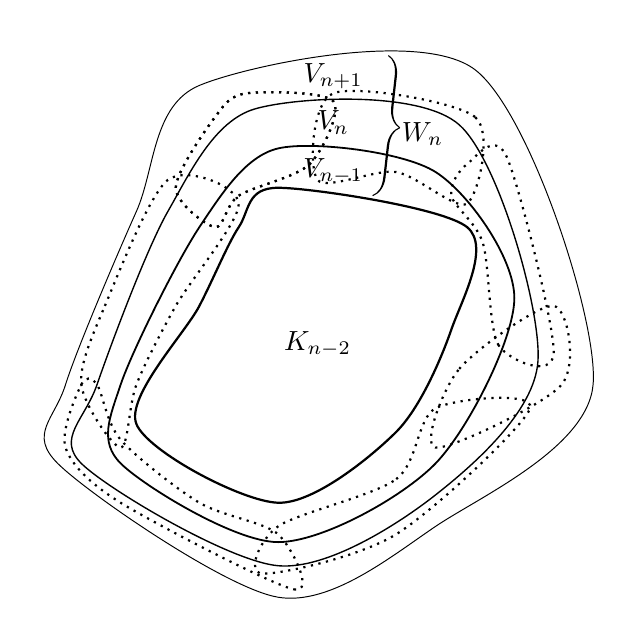
\begin{tikzpicture}
            \draw[line width=0.35] plot[smooth cycle] coordinates {
                    (-0.8,1) (2,-0.7) (4,0.2) (6,2) (4.5,6) (1,5.8) (0.2,4.2) (-0.7,2)
                };
            \draw[line width=0.5] plot[smooth cycle] coordinates {
                    (-0.5,1) (2,-0.3) (4,0.6) (5.3,2.3) (4.3,5.3) (1.7,5.5) (0.6,4.2) (-0.3,2)
                };
            \draw[line width=0.65] plot[smooth cycle] coordinates {
                    (0,1) (2,0) (4,1) (5,3.1) (4,4.7) (2,5) (1,4) (0,2)
                };
            \draw[thick] plot[smooth cycle] coordinates {
                    (0.2,1.5) (2,0.5) (3.5,1.4) (4.2,2.7) (4.4,4) (2,4.5) (1.5,4) (1,3)
                };
            \draw[thick, dotted] plot[smooth cycle] coordinates {
                    (4.4,4.3) (4.5,5.4) (2.7,5.7) (2.5,4.6) (3.5,4.7)
                };
            \draw[thick, dotted] plot[smooth cycle] coordinates {
                    (1.2,4) (0.7,4.5) (1.2,5.4) (1.6,5.7) (2.7,5.6) (2.4,4.8) (1.5,4.4)
                };
            \draw[thick, dotted] plot[smooth cycle] coordinates {
                    (1.2,4) (0.7,4.5) (1.2,5.4) (1.6,5.7) (2.7,5.6) (2.4,4.8) (1.5,4.4)
                };
            \draw[thick, dotted] plot[smooth cycle] coordinates {
                    (-0.5,2) (-0.2,3) (0.6,4.6) (1.5,4.3) (0.7,3) (0.2,2) (0,1.2)
                };
            \draw[thick, dotted] plot[smooth cycle] coordinates {
                    (0,0.5) (2.2,-0.6) (2,0.1) (1,0.5) (0,1.3) (-0.3,2) (-0.5,2) (-0.7,1.2)
                };
            \draw[thick, dotted] plot[smooth cycle] coordinates {
                    (2,0.2) (3.5,0.8) (4,1.7) (5.2,1.7) (3.5,0.1) (1.8,-0.4)
                };
            \draw[thick, dotted] plot[smooth cycle] coordinates {
                    (4,1.2) (4.3,2.2) (5.5,3) (5.6,2)
                };
            \draw[thick, dotted] plot[smooth cycle] coordinates {
                    (5.5,2.4) (4.8,2.5) (4.6,3.8) (4.2,4.4) (4.4,4.8) (4.9,4.9)
                };

            \node[anchor=north] at (2.5,2.8) {\(K_{n-2}\)};
            \node[anchor=north] at (2.7,5) {\(V_{n-1}\)};
            \node[anchor=north] at (2.7,5.6) {\(V_n\)};
            \node[anchor=north] at (2.7,6.2) {\(V_{n+1}\)};
            \draw[decorate,decoration={calligraphic
                        brace, amplitude=7pt},thick] (3.4,6.18) -- (3.2,4.4) node[midway, yshift=-3pt,right=4pt] {\(W_n\)};
        \end{tikzpicture}
        \caption{The geometry of the finite subcover of \(V_n\subset W_n\) for some \(n\in\mathbb{N}\).}
        \label{fig:locallyfiniteopencoverexistence}
    \end{figure}Let \(K_{-1}=K_0=\emptyset,K_1,K_2,\cdots\subset\Omega\) exhaust \(\Omega\), with each \(K_n\) compact and \(K_n\subseteq K_{n+1}^\circ\). For each \(n\in\mathbb{N}\), define \(W_n=K_{n+1}^\circ\setminus K_{n-2}\), which is open, and \(V_n=K_n\setminus K_{n-1}^\circ\), which is compact (as in \autoref{fig:locallyfiniteopencoverexistence}).

    By construction, \(V_n\subseteq W_n\) for all \(n\in\mathbb{N}\). The sets \(\{V_n\}\) form compact shells exhausting \(\Omega\), since \(\bigcup_{n\in\mathbb{N}}V_n=\Omega\).

    \(\forall n\in\mathbb{N}\) and \(\forall z\in V_n\), since \(W_n\) is an open set containing \(z\) and \(\mathfrak{B}\) is a basis, there exists \(U_{z,n}\in\mathfrak{B}\) such that \(z\in U_{z,n}\subseteq W_n\) (in short, \(U_{z,n}\) is an open neighborhood of \(z\) that is contained in \(W_n\)). The collection \(\cbraces{U_{z,n}}{z\in V_n}\) is an open cover of the compact set \(V_n\), so by the Heine-Borel Theorem (\autoref{thm:heineborel}) it admits a finite subcover of \(V_n\), as pictured in the dotted lines of \autoref{fig:locallyfiniteopencoverexistence}. That is, there exist finitely many points \(z_{n,1},\ldots,z_{n,k_n}\) such that \(V_n\subset\bigcup_{i=1}^{k_n}U_{z_{n,i},n}\subseteq W_n\).

    Let \(\{U_j\}\) be the collection formed by enumerating all such \(U_{z_{n,i},n}\) for \(n\in\mathbb{N}\) and \(i=1,\ldots,k_n\). Then \(\{U_j\}\subset\mathfrak{B}\) is a countable collection whose union covers \(\Omega\), proving \ref{itm:locallyfiniteopencoverexistence_cover}.

    For \ref{itm:locallyfiniteopencoverexistence_localfiniteness}, let \(K\subset\Omega\) be compact. Then \(\exists N\in\mathbb{N}\) such that \(K\subset K_N^\circ\), and hence \(K\) is disjoint from \(V_n\) for all \(n>N+1\). Since each \(V_n\) intersects only finitely many \(U_j\), it follows that \(K\) intersects only finitely many of the \(U_j\). Thus, the collection is \textit{locally finite}.
\end{proof}
\begin{remark}
    The property of local finiteness of an open collection \(S\) in \(\Omega\) is commonly stated as:

    \(\forall z\in\Omega\), there exists an open neighborhood of \(z\) intersecting finitely many sets in \(S\).

    Obviously, this assertion implies \ref{itm:locallyfiniteopencoverexistence_localfiniteness} in \autoref{lemma:locallyfiniteopencoverexistence}: let \(K\subset \Omega\) be compact, and for every \(z\in\Omega\), the collection of neighborhoods covers \(K\), and by compactness, admits a finite subcover. Therefore, \(K\) intersects finitely many sets in \(S\). Conversely, \(\forall z\in\Omega\), there exists an open neighborhood \(V\ni z\) relatively compact in \(\Omega\). By assumption, \(\overline{V}\) intersects finitely many sets in \(S\), and since \(V\subset\overline{V}\), the conclusion follows.
\end{remark}
\begin{theorem}[Partition of Unity]\label{thm:partitionofunity}
    For a nonempty open set \(\Omega\subseteq\mathbb{C}\), let \(\cbraces{\Omega_k}_{k\in\mathbb{Z}_{\ge0}}\) be an open cover of \(\Omega\). Then there exists a set of bump functions, \(\alpha_1(z),\alpha_2(z),\ldots\in C^\infty(\mathbb{C})\) with compact support within \(\Omega\) satisfying
    \begin{enumerate}
        \item \(\forall j\in\mathbb{N}\), \(\exists k\in\mathbb{Z}_{\geq0}\) such that \(\supp\paren{\alpha_j}\subseteq\Omega_k\).\label{itm:partitionofunity_subordinate}
        \item The collection \(\qty{\supp\paren{\alpha_j}}\) is locally finite.\label{itm:partitionofunity_localfiniteness}
        \item \(\forall j\in\mathbb{N}\), \(0\leq\alpha_j\leq 1\).\label{itm:partitionofunity_nonnegativity}
        \item \(\forall z\in\Omega\), \(\sum_{j=1}^\infty \alpha_j(z)=1,\)\label{itm:itm:partitionofunity_partitionofunity}
    \end{enumerate} known as a \(C^\infty\) partition of unity subordinate to \(\cbraces{\Omega_k}_{k\in\mathbb{Z}_{\geq0}}\).
\end{theorem}
\begin{proof}
    By the openness of \(\Omega_k\), \(\forall z\in\Omega\), \(\exists r_z>0\) such that \(\overline{D\paren{z,r_z}}\subset\Omega_{k_z}\) for some \(k_z\in\mathbb{Z}_{\ge0}\).

    Then, \(\cbraces{D\paren{z,r}}{z\in\Omega, 0<r<r_z}\) forms an open basis of \(\Omega\). Then by \autoref{lemma:locallyfiniteopencoverexistence}, there exists a locally finite open cover \(\cbraces{D\paren{z_j,r_{z_j}}}\) of \(\Omega\), and since it is a subcollection of the basis, \[D\paren{z_j,r_{z_j}}\subset\overline{D\paren{z_j,r_{z_j}}}\subset\Omega_{k_{z_j}},\quad\forall j\in\mathbb{N}.\] The most trivial bump function has the form \[\theta(z)=\begin{cases}
            \exp\paren{\frac{1}{\abs{z}^2-1}} & \abs{z}<1   \\
            0                                 & \abs{z}\ge1
        \end{cases},\] which has the support \(\overline{D(0,1)}\). Define the function \(\theta_\varepsilon(z)=\varepsilon^{-2}\theta\qty(\frac{z}{\varepsilon})\) with the support \(\overline{D(0,\varepsilon)}\), which satisfies that \(\forall\varepsilon>0\), \[\int_{\mathbb{C}}\theta_\varepsilon(z)\ddx\wedge\ddy=1.\]
    Define a set of functions \(\cbraces{\beta_j(z)}_{j\in\mathbb{N}}\) with \(\beta_j(z)=\theta_{r_{z_j}}\paren{z-z_j}\), which is a bump function with \(\supp\qty(\beta_j)=\overline{D\paren{z_j, r_{z_j}}}\subset\Omega_{k_{z_j}}\).

    By the local finiteness of \(\qty{D\qty(z_j,r_{z_j})}\), there exists an open neighborhood \(V_z\) of each point \(z\in\Omega\) such that the set \(\cbraces{j}{V_z\cap D\qty(z_j,r_{z_j})\neq\emptyset}\) is finite. Since every open neighborhood of each point in \(\overline{D\qty(z_j,r_{z_j})}\) intersects \(D\qty(z_j,r_{z_j})\), it follows that every open set disjoint from \(D\qty(z_j,r_{z_j})\) is also disjoint from its closure. Since \(\overline{D\qty(z_j,r_{z_j})}\supset D\qty(z_j,r_{z_j})\), any open set intersecting \(D\qty(z_j,r_{z_j})\) will intersect \(\overline{D\qty(z_j,r_{z_j})}\). Therefore, \(\cbraces{j}{V_z\cap\overline{D\qty(z_j,r_{z_j})}\neq\emptyset}\) is finite. Equivalently, \(\cbraces{\supp\paren{\beta_j}}_{j\in\mathbb{N}}\) is locally finite on \(\Omega\).

    Consequently, \(\forall z_0\in\Omega\), there exists an open neighborhood \(V\ni z_0\) that intersects a finite number of sets in \(\cbraces{\supp\paren{\beta_j}}_{j\in\mathbb{N}}\). Then \(\forall z\in V\), the sum \[S(z)=\sum_{j=1}^\infty\beta_j(z)\] is a sum of finitely many terms and is therefore \(C^\infty\) at \(z_0\). Since the collection of supports exhausts \(\Omega\), \(S(z)\) is positive. Therefore, the sequence defined by \[\alpha_j(z)={\frac{\beta_j(z)}{S(z)}}\] is also \(C^\infty\) and is compactly supported in \(\Omega\). Furthermore, it satisfies \[\sum_{j=1}^\infty\alpha_j(z)=1.\]
\end{proof}
\begin{theorem}[Existence of Bump Functions]\label{thm:bumpfunctionexistence}
    Let \(\Omega\subset\mathbb{C}\) be open, \(K\subset\Omega\) be compact, and \(V\subseteq\Omega\) be an open neighborhood of \(K\). Then there exists a bump function \(\varphi\in C^\infty\paren{\mathbb{C}}\) with compact support contained in \(V\) such that \(\forall z\in\mathbb{C}\), \(0\leq\varphi(z)\leq 1\), and there exists an open neighborhood of \(K\) over which \(\varphi\equiv1\).
\end{theorem}
\begin{proof}
    Let \(V(K,\varepsilon)=\left\{z\in\mathbb{C}\,\middle|\,\inf_{\zeta\in K}\abs{\zeta-z}<\varepsilon\right\}\). In other words, \(z\) is within \(\varepsilon\) apart from \(K\).

    Then \(\exists\varepsilon>0\) such that \(K\subset V(K,\varepsilon)\subset V(K,2\varepsilon)\subseteq V\). Let \(\Omega_1=V(K,2\varepsilon)\) and \(\Omega_2=\Omega\setminus V(K,\varepsilon)\). Then there exists a \(C^\infty\) partition of unity \(\cbraces{\alpha_j(z)}_{j\in\mathbb{N}}\) of \(\Omega\) subordinate to the open cover \(\cbraces{\Omega_1,\Omega_2}\). Define a new function
    \[\varphi(z)=\sum_{\substack{j\in\mathbb{N}\\\supp{\alpha_j}\subseteq\Omega_1}}\alpha_j(z).\]
    It follows that \(\varphi\in C^\infty(\mathbb{C})\) with compact support in \(\Omega_1\). Since the support of every \(\alpha_j\) where \(j\in\mathbb{N}\) lies entirely either in \(\Omega_1\) or \(\Omega_2\), \[1=\sum_{\substack{j\in\mathbb{N}\\\supp{\alpha_j}\subseteq\Omega_2}}\alpha_j(z)+\varphi(z).\]
    When \(z\in\Omega_1\setminus\Omega_2=V(K,\varepsilon)\), the first summation vanishes, meaning that \(\varphi(z)\equiv1\) on the neighborhood \(V(K,\varepsilon)\) of \(K\). When \(z\in\Omega_2\setminus\Omega_1=\Omega\setminus V(K,2\varepsilon)\), \(\varphi(z)\) vanishes.
\end{proof}
\subsection{Zeros of a Holomorphic Function}
For a region \(U\subseteq\mathbb{C}\) and a holomorphic function \(f:U\to\mathbb{C}\), a point \(z_0\in U\) is a \textit{zero} of \(f\) if and only if \(f\paren{z_0}=0\). Furthermore, if \(f\) has the Taylor expansion at \(z_0\) of \[a_m\paren{z-z_0}^m+a_{m+1}\paren{z-z_0}^{m+1}+\cdots,\qquad m\in\mathbb{N},a_m\neq0,\] then the zero at \(z_0\) has multiplicity \(m\).

We will introduce a fundamental application of Liouville's Theorem (\autoref{thm:liouville}) below.
\begin{theorem}[Fundamental Theorem of Algebra]\label{thm:fundamentaltheoremofalgebra}
    Every non-constant polynomial \(p(z)\) with complex coefficients has at least one complex zero.
\end{theorem}
\begin{proof}
    For the sake of contradiction, suppose that \(p(z)\) has no complex zeros. Then the function \(f(z)=\frac{1}{p(z)}\) is continuous and entire, because \(p(z)\) has no zeros in \(\mathbb{C}\). Moreover, as \(|z|\to\infty\), \(p(z)\to\infty\), so \(f(z)\to 0\), and thus \(f(z)\) is bounded. By Liouville's Theorem (\autoref{thm:liouville}), every bounded entire function is constant. Thus, \(f(z)\) is constant, and so \(p(z)\) must also be constant. By contradiction, \(p(z)\) has at least one complex zero.
\end{proof}
\begin{theorem}\label{thm:identityaccumulationofzeros}
    Let \(U\subseteq\mathbb{C}\) be open and connected, and \(f:U\to\mathbb{C}\) be holomorphic over \(U\). Then if the set defined by \(S=\cbraces{z\in U\mid f(z)=0}\) has an accumulation point in \(U\), then \(f\equiv0\) over \(U\).
\end{theorem}
\begin{proof}
    Let \(\cbraces{z_n}_{n\in\mathbb{N}}\) be a subset of \(S\) and assume it has an accumulation point \(z_\infty\) in \(U\). Since \(f\) is holomorphic over \(U\), \(\exists\varepsilon>0\) such that \(f\) is holomorphic over \(D\paren{z_\infty,\varepsilon}\subseteq U\). Then over this disk, \(f\) has the Taylor expansion
    \begin{equation}\label{eq:identityaccumulationofzeros_taylorexpansion}
        f(z)=\sum_{n=0}^\infty a_n\paren{z-z_\infty}^n.
    \end{equation}
    By \autoref{def:accumulationpoint}, \(\exists N\in\mathbb{N}\) such that \(\forall n>N\), \(z_n\in D\paren{z_\infty,\varepsilon}\). Since \(z_n\) is a zero of \(f\), \(f\paren{z_n}=0\). Then, by the continuity of \(f\), \[\lim_{n\to\infty} f\paren{z_n}=f\paren{\lim_{n\to\infty}z_n}=f\paren{z_\infty}=0.\] Using this result in comparison to equation~\eqref{eq:identityaccumulationofzeros_taylorexpansion}, we get that \(a_0=0\).

    The function \(f_1(z)=\frac{f(z)}{z-z_\infty}\) has a Taylor expansion over \(D\paren{z_0,\varepsilon}\) of
    \[f_1(z)=\sum_{n=0}^\infty a_{n+1}\paren{z-z_\infty}^n.\]
    Let \(z=z_n\neq z_\infty\) for some \(n>N\). Then \(f_1\) vanishes, leaving \[0=a_1+\mathcal{O}_{n\to\infty}\paren{z_n-z_\infty}.\]
    Letting \(n\to\infty\), \(z_n\to z_\infty\), and \(a_1=0\). Define \(f_2(z)=\frac{f_1(z)}{z-z_\infty}\). Then, \[f_2(z)=\sum_{n=0}^\infty a_{n+2}\paren{z-z_\infty}^n.\]
    Similarly, \(a_2=0\). Letting \(f_n(z)=\frac{f(z)}{\paren{z-z_\infty}^n}\), the sequence \(\cbraces{a_n}_{n\in\mathbb{Z}_{\geq0}}\) vanishes, and \(f\equiv 0\) on \(D\paren{z_\infty,\varepsilon}\).

    Let \(S^*=\cbraces{z\in U}{\forall n\in\mathbb{Z}_{\geq0}, f^{(n)}(z)=0}\). \(\forall z\in D\paren{z_\infty,\varepsilon}\), since \(f(z)\) locally vanishes (and has vanishing derivatives as a consequence), \(D\paren{z_\infty,\varepsilon}\subseteq S^*\). Furthermore, \(\forall z'\in S^*\), \(\exists\varepsilon'>0\) such that \(f(z)\) has a convergent Taylor series with vanishing coefficients on \(D(z',\varepsilon')\subseteq U\). Then \(f\equiv0\) on \(D\paren{z',\varepsilon'}\). Then \(\forall z\in D(z',\varepsilon')\), since \(f\) is constant at \(z\), it also has vanishing derivatives. It follows that \(D(z',\varepsilon')\subseteq S^*\). Since every point in \(S^*\) has an open neighborhood also in \(S^*\), \(S^*\) is open.

    \(\forall k\in\mathbb{Z}_{\geq0}\), \(f^{(k)}\) is continuous in \(U\) by the holomorphy of \(f\). Let \(S_k=\cbraces{z\in U}{f^{(k)}(z)=0}\). For any sequence \(\cbraces{z'_n}\in S_k\) converging to some \(z'_\infty\in U\), by the continuity of \(f\), \[\lim_{n\to\infty} f^{(k)}\paren{z'_n}=f^{(k)}\paren{\lim_{n\to\infty}z'_n}=f^{(k)}\paren{z'_\infty}=0,\] and therefore \(z'_\infty\in S_k\). Thus, \(S_k\) contains all of its accumulation points in \(U\) and is therefore closed in \(U\) (if \(z'_\infty\notin U\), then it is no longer relevant; we are concerned about it being closed within \(U\)). Since \(S^*=\bigcap_{k\in\mathbb{Z}_{\geq0}} S_k\) and each of \(S_k\) is closed in \(U\), \(S^*\) is the intersection of closed sets and consequently closed.

    Since \(S^*\) is nonempty and clopen in the connected set \(U\), \(S^*=U\) (by \autoref{thm:connectedtopologicalspaceclopensets}). It follows that \(f\equiv 0\) on \(U\).
\end{proof}
\begin{remark}
    This is a trivial property of holomorphic functions that allows for the uniqueness of analytic continuations. It is oftentimes stated in the form below:
\end{remark}
\begin{theorem}[Identity Theorem]\label{thm:identity}
    Let \(U\subseteq\mathbb{C}\) be open and connected, and define \(f(z)\) and \(g(z)\) to be two holomorphic functions on \(U\). For a set \(S\subseteq U\) with an accumulation point in \(U\), if \(f\equiv g\) on \(S\), then \(f\equiv g\) on \(U\).
\end{theorem}
\begin{proof}
    Let \(h=f-g\) be holomorphic over \(U\). Since \(S\) has an accumulation point in \(U\), and \(h\equiv 0\) over \(S\), then by \autoref{thm:identityaccumulationofzeros}, \(h\equiv 0\) over \(U\).
\end{proof}
\begin{theorem}[Argument Principle for Holomorphic Functions]\label{thm:argumentprincipleholomorphic}
    Let \(U\subseteq\mathbb{C}\) be a region and \(f:U\to\mathbb{C}\) be holomorphic. Let \(\gamma\subset U\) be a closed, positively oriented curve homotopic to a constant curve (the homotopy completely lies in \(U\)). If \(f\) has no zeros on \(\gamma\), then \(f\) has finitely many zeros in the region bounded by \(\gamma\) and this number, counting multiplicities, is equal to \[k=\frac{1}{2\pi i}\int_{\gamma}\frac{f'(z)}{f(z)}\ddz.\]
    Let \(\Gamma\) be the image of \(\gamma\) under \(f\). Then, \(k=\frac{1}{2\pi}\Delta_\Gamma\arg(f)\), where \(\Delta_\Gamma\arg(f)=\Delta_{\gamma}\arg(f(z))\) is the total change in argument of \(f(z)\) as \(z\) traverses \(\gamma\).
\end{theorem}
\begin{proof}
    Let \(z_1,z_2,\ldots,z_n\) be the zeros enclosed within \(\gamma\), with multiplicities \(k_1,k_2,\ldots,k_n\) respectively. There exist disks centered around each zero with radii \(\varepsilon_1,\ldots,\varepsilon_n\) respectively, such that each disk is disjoint and contained in the interior of \(\gamma\). The function \[\frac{f'(z)}{f(z)}\] is holomorphic over \[\mathrm{int}\paren{\gamma}\setminus\bigcup_{j=1}^n D\paren{z_j,\varepsilon_j},\] where \(\mathrm{int}\paren{\gamma}\) is the interior with respect to the Jordan curve \(\gamma\).
    This region has the oriented boundary of \(\bigcup_{j=1}^n\partial D\paren{z_j,\varepsilon_j}^-\cup\gamma^+\). By the Cauchy--Goursat Integral Theorem (\autoref{thm:cauchygoursattheorem}), \[\int_{\bigcup_{j=1}^n\partial D\paren{z_j,\varepsilon_j}^-\cup\gamma^+}\frac{f'(z)}{f(z)}\ddz=0,\]
    and from rearrangement, \[\int_\gamma \frac{f'(z)}{f(z)}\ddz=\sum_{j=1}^n\int_{\partial D\paren{z_j,\varepsilon_j}}\frac{f'(z)}{f(z)}\ddz.\]
    Since \(z_j\) has multiplicity \(k_j\), \(f(z)\) can be locally (over the disk) written as \(\paren{z-z_j}^{k_j}h_j(z)\), where \(\forall z\in D\paren{z_j,\varepsilon_j}\), \(h_j\paren{z}\neq 0\). Analyzing the integrand's numerator,
    \[f'(z)=k_j\paren{z-z_j}^{k_j-1}h_j(z)+\paren{z-z_j}^{k_j}h_j'(z),\]
    and the integrand is equal to
    \[\frac{f'(z)}{f(z)}=\frac{k_j}{z-z_j}+\frac{h_j'(z)}{h_j(z)}.\]
    Notice that \(h_j(z)\) may not vanish on \(\partial D\paren{z_j,\varepsilon_j}\) either, as otherwise, \(f\) would be a zero on \(\partial D\paren{z_j,\varepsilon_j}\), and there would not be a disjoint disk centered at the zero. Thus,
    \[\sum_{j=1}^n\int_{\partial D\paren{z_j,\varepsilon_j}}\frac{f'(z)}{f(z)}\ddz=\sum_{j=1}^n\int_{\partial D\paren{z_j,\varepsilon_j}}\brackets{\frac{k_j}{z-z_j}+\frac{h_j'(z)}{h_j(z)}}\ddz.\] Once again applying \autoref{thm:cauchygoursattheorem}, the second term vanishes when integrating, and by the Cauchy--Goursat Integral Formula (\autoref{thm:cauchygoursatformula}), \[\int_{\gamma}\frac{f'(z)}{f(z)}\ddz=\sum_{j=1}^n\int_{\partial D\paren{z_j,\varepsilon_j}}\frac{k_j}{z-z_j}\ddz=2\pi i\sum_{j=1}^n k_j=2\pi ik.\]
    Letting \(f=f(z)\), through substitution, \[k=\frac{1}{2\pi i}\int_\Gamma \frac{1}{f}\dd{f}=\frac{1}{2\pi i}\Delta_\Gamma\log(f)=\frac{1}{2\pi}\Delta_\Gamma\arg(f).\]
\end{proof}
This profound result proves that the number of zeros of a holomorphic function enclosed by a closed curve is also the number of times the image of the curve winds around the origin.
\begin{theorem}\label{thm:hurwitzsimplecase}
    Let \(\cbraces{f_n(z)}\) be a sequence of holomorphic functions on the open set \(U\subseteq\mathbb{C}\) that uniformly converges to \(f(z)\) on every compact subset of \(U\). If \(\forall n\in\mathbb{N}\), \(f_n(z)\) has no zeros in \(U\), then \(f\) is either identically 0 or has no zeros in \(U\).
\end{theorem}
\begin{proof}
    By the holomorphy of \(f_n(z)\), for any simple closed rectifiable curve \(\gamma\subset U\) (whose interior is a subset of \(U\)), by the Cauchy--Goursat Integral Theorem (\autoref{thm:cauchygoursattheorem}), \[\int_{\gamma}f_n(\zeta)\ddzeta=0.\] Since \(\gamma\) is a subset of any compact subset of \(U\), \(\cbraces{f_n(\zeta)}\) uniformly converges on \(\gamma\), and by \autoref{thm:limitintegralswitch}, \begin{equation}
        \lim_{n\to\infty}\int_{\gamma}f_n(\zeta)\ddzeta=\int_{\gamma}\lim_{n\to\infty}f_n(\zeta)\ddzeta=\int_{\gamma}f(\zeta)\ddzeta=0.\label{eq:hurwitzsimplecase_integrallimitswitchforholomorphy}
    \end{equation}
    Then by Morera's Theorem (\autoref{thm:morera}), \(f(z)\) is holomorphic, and \(f'(z)\) is holomorphic. We aim to show that \(f'_n(z)\rightrightarrows f'(z)\).

    Let \(K\subset U\) be arbitrary and compact and \(V\supset K\) be open and relatively compact in \(U\). Since \(\cbraces{f'_n(z)}\) is holomorphic, by \autoref{crl:nthderivativeboundedsupremum}, there exists a finite constant \(c>0\) such that \[\lim_{n\to\infty}\sup_{z\in K}\abs{f'_n(z)-f'(z)}\leq c\lim_{n\to\infty}\sup_{z\in V}\abs{f_n(z)-f(z)}.\]

    By the definition of uniform convergence, the right-hand side approaches 0, and \(\cbraces{f'_n(z)}\) is then uniformly convergent to \(f'(z)\) by the same reasoning.

    Through the proof of \autoref{thm:identityaccumulationofzeros}, if \(f\not\equiv0\) over \(U\), then the zeros of \(f\) do not have an accumulation point in \(U\) and are therefore discrete. In this case, let \(\gamma\subset U\) be a curve that does not pass through the zeros of \(f\). Since each function in the sequence \(f_n\) does not contain zeros in \(U\), by the Argument Principle, (\autoref{thm:argumentprincipleholomorphic}),
    \begin{equation}
        \lim_{n\to\infty}\int_{\gamma}\frac{f_n'(z)}{f_n(z)}\ddz=0.\label{eq:hurwitzsimplecase_argumentprinciple}
    \end{equation}
    Since \(f\) and \(f'\) are holomorphic over \(\gamma\), by \autoref{thm:continuousfunctionboundedoncompact}, there exists a finite value \(M>0\) such that \(\forall z\in\gamma\), \(\max\paren{\abs{f(z)},\abs{f'(z)}}<M\).

    Since \(\gamma\) does not pass through the zeros of \(f\), \(\exists\lambda>0\) such that \(\forall z\in\gamma\), \(\abs{f(z)}>\lambda\). By the uniform convergence of \(\cbraces{f_n(z)}\), \(\exists N\in\mathbb{N}\) such that
    \[\abs{f_n(z)-f(z)}<\frac{\lambda}{2},\quad\forall n>N,\forall z\in\gamma.\]
    Then \(\abs{f_n(z)}>\frac{\lambda}{2}\) on \(\gamma\). It follows that \(\frac{1}{f_n(z)}\) and its limit are uniformly bounded: \[\abs{\frac{1}{f(z)}}<\frac{1}{\lambda},\quad\abs{\frac{1}{f_n(z)}}<\frac{2}{\lambda},\quad\forall z\in\gamma,\forall n>N.\]
    Then,
    \begin{align*}
        \abs{\frac{f'}{f}-\frac{f'_n}{f_n}}                                               & =\abs{\frac{f'f_n-f'_nf}{f_nf}}                                                                                                           \\
                                                                                          & <2\frac{\abs{f'f_n-f'f}+\abs{f'f-f'_nf}}{\lambda^2}                                                                                       \\
                                                                                          & <\frac{2M}{\lambda^2}\cdot\paren{\abs{f_n-f}+\abs{f'-f'_n}}.                                                                              \\
        \sup_{z\in\gamma}\abs{\frac{f'(z)}{f(z)}-\frac{f'_n(z)}{f_n(z)}}                  & \leq\frac{2M}{\lambda^2}\paren{\sup_{z\in\gamma}\abs{f_n(z)-f(z)}+\sup_{z\in\gamma}\abs{f'(z)-f'_n(z)}}                                   \\
        \lim_{n\to\infty}\sup_{z\in\gamma}\abs{\frac{f'(z)}{f(z)}-\frac{f'_n(z)}{f_n(z)}} & \leq\frac{2M}{\lambda^2}\paren{\lim_{n\to\infty}\sup_{z\in\gamma}\abs{f_n(z)-f(z)}+\lim_{n\to\infty}\sup_{z\in\gamma}\abs{f'(z)-f'_n(z)}} \\
                                                                                          & =0.
    \end{align*}
    Therefore, \(\frac{f'(z)}{f(z)}\) is uniformly convergent on \(\gamma\). Then we can pass the limit through the integral in equation~\eqref{eq:hurwitzsimplecase_argumentprinciple}. Then,
    \[\lim_{n\to\infty}\int_\gamma \frac{f'_n(z)}{f_n(z)}\ddz=\int_\gamma \frac{f'(z)}{f(z)}\ddz=0.\] By the Argument Principle, (\autoref{thm:argumentprincipleholomorphic}), \(f(z)\) has no zeros in the interior of \(\gamma\). Since \(\gamma\) was arbitrarily chosen, either \(f(z)\equiv 0\) on \(U\) or has no zeros in \(U\).
\end{proof}
\begin{theorem}[Rouché's Theorem]\label{thm:rouche}
    Let \(U\subseteq\mathbb{C}\) be open and \(f,g\) be two holomorphic functions over \(U\). Let \(\gamma\subset U\) be a simple, closed, rectifiable curve, and \(\forall z\in\gamma\)
    \begin{equation}
        \abs{f(z)-g(z)}<\abs{f(z)}\label{eq:rouche}.
    \end{equation} Then \(f\) and \(g\) have the same number of zeros enclosed by \(\gamma\).
\end{theorem}
\begin{proof}
    It is obvious that \(g(z)\) has no zeros on \(\gamma\). Otherwise, \(\exists z_0\in\gamma\) such that \(g\paren{z_0}=0\), implying that \(\abs{f\paren{z_0}}<\abs{f\paren{z_0}}\) which is impossible.

    Let \(k_f\) and \(k_g\) denote the number of zeros of \(f\) and \(g\) enclosed by \(\gamma\), respectively. By the Argument Principle (\autoref{thm:argumentprincipleholomorphic}),
    \[k_g-k_f=\int_{\gamma}\frac{g'(z)}{g(z)}\ddz-\int_\gamma\frac{f'(z)}{f(z)}\ddz=\int_\gamma\frac{g'(z)f(z)-f'(z)g(z)}{g(z)f(z)}\ddz=\int_\gamma\frac{\qty(\dfrac{g(z)}{f(z)})'}{\dfrac{g(z)}{f(z)}}\ddz.\]

    Let \(w=h(z)=\frac{g(z)}{f(z)}\) with \(\Gamma=h(\gamma)\). Then, \[k_g-k_f=\int_\Gamma\frac{\dd{w}}{w}.\]
    From equation~\eqref{eq:rouche}, by dividing both sides by \(f(z)\), we obtain \(\abs{w-1}<1\). Then \(\Gamma\) lies in the open disk \(D(1,1)\), which will never intersect or enclose 0. Then by \autoref{lemma:cauchyintegraltheoremoversimplyconnectedset}, \[k_g-k_f=\int_\Gamma\frac{\dd{w}}{w}=0,\] as desired.
\end{proof}
By the Fundamental Theorem of Algebra (\autoref{thm:fundamentaltheoremofalgebra}), any polynomial in the form \(p(z)=\sum_{k=0}^n a_kz^k\) (\(n\in\mathbb{N}\), \(a_n\neq 0\), \(a_k\in\mathbb{C}\) where \(k=1,\ldots n\)) has at least one complex zero. Consider the function \(q(z)=a_nz^n\), with a zero at \(z=0\) with multiplicity \(n\). By Rouché's Theorem (\autoref{thm:rouche}), since \(\exists R\in\mathbb{R}\) such that \(\abs{q(z)-p(z)}=\abs{\sum_{k=0}^{n-1}a_kz^k}<\abs{a_nz^n}\) over \(\abs{z}=R\), \(p\) and \(q\) have the same number of zeros, counting multiplicity.

\autoref{thm:hurwitzsimplecase} is a specific case of the following theorem:
\begin{theorem}[Hurwitz's Theorem]\label{thm:hurwitz}
    Let \(\cbraces{f_n(z)}\) be a sequence of holomorphic functions on the open set \(U\subseteq\mathbb{C}\) that uniformly converges to \(f(z)\) on every compact subset of \(U\) such that \(f\not\equiv0\) over \(U\).

    Then, for any compact set \(K\subset U\) where \(f(z)\) has no zeros on \(\partial K\), and any open neighborhood \(V\) of the set \(\cbraces{z\in K}{f(z)=0}\), \(\exists N\in\mathbb{N}\) such that \(\forall n>N\),
    \begin{enumerate}
        \item The zeros of \(f_n(z)\) in \(K\) lie in \(V\), that is, \(\cbraces{z\in K}{f_n(z)=0}\subset V\).
        \item The number of zeros (counting multiplicity) of \(f_n(z)\) in \(K\) is the same as that of \(f(z)\) in \(K\).
    \end{enumerate}
\end{theorem}
\begin{proof}
    By the same logic as with the proof of \autoref{thm:hurwitzsimplecase}, \(f(z)\) is holomorphic over \(U\). Since \(f\not\equiv 0\) on \(U\), its zeros in \(K\), \(\cbraces{z_j}\), are isolated.

    Since \(f\) does not vanish on \(\partial K\), \(\abs{f}\) attains its positive infimum on \(\partial K\). Since \(f_n\rightrightarrows f\) over \(\partial K\) (as it is a compact subset of \(U\)), \(\exists N_1\in\mathbb{N}\) such that \[\abs{f(z)-f_n(z)}<\abs{f(z)},\quad\forall z\in \partial K,\forall n>N_1.\] By Rouché's Theorem (\autoref{thm:rouche}), \(f\) and \(f_n\) have the same number of zeros (counting multiplicities) in \(K\).

    The function \(f\) has no zeros in \(K\setminus V\) (as \(V\) contains all zeros of \(f\) in \(K\)). Since \(K\setminus V\) is compact, \(|f|\) attains a positive minimum, and \(f_n\rightrightarrows f\) on this set. Similarly, \(\exists N_2\in\mathbb{N}\) such that \(\forall n>N_2\), \[\abs{f(z)-f_n(z)}<\abs{f(z)},\quad\forall z\in K\setminus V.\]
    \(K\setminus V\) can be covered by a collection of simply connected sets (with a union equal to \(K\setminus V\)). Thus, by \autoref{thm:rouche}, \(f\) and \(f_n\) never vanish on \(K\setminus V\), and therefore all zeros of \(f_n\) lie in \(V\).

    For the purpose of the statement, we can choose \(N=\max\paren{N_1,N_2}\).
\end{proof}
The following theorem is also a direct consequence of Rouché's Theorem (\autoref{thm:rouche}). While \autoref{thm:hurwitz} concerns the stability of zeros under perturbations of \(f_n(z)\) as \(n\) increases, the stability is also preserved under small additive perturbations of the form \(f(z)+\lambda\) for vanishing \(\lambda\). Observe their similarities in formulation.
\begin{theorem}\label{thm:holomorphiczerosstabilityundershifts}
    Let \(U\subseteq\mathbb{C}\) be open and connected, and \(f(z)\) be holomorphic and non-constant on \(U\).

    Then, for any compact set \(K\subset U\) where \(f(z)\) has no zeros on \(\partial K\), and any open neighborhood \(V\) of the set \(\cbraces{z\in K}{f(z)=0}\), \(\exists \delta>0\) such that \(\forall\lambda\in D\paren{0,\delta}\),
    \begin{enumerate}
        \item The zeros of \(f(z)+\lambda\) in \(K\) lie in \(V\), that is, \(\cbraces{z\in K}{f(z)+\lambda=0}\subset V\).
        \item The number of zeros (counting multiplicity) of \(f(z)+\lambda\) in \(K\) is the same as that of \(f(z)\) in \(K\).
    \end{enumerate}
\end{theorem}
\begin{proof}
    The proof is exactly the same as in \autoref{thm:hurwitz}. Obviously, \(|f|\) attains its positive infimum on \(\partial K\) by its continuity, or that \(\delta_1=\min_{z\in\partial K}\abs{f(z)}\) is positive. Then \(\forall\abs{\lambda}<\delta_1\), \(\forall z\in \partial K\),
    \[\abs{f(z)-\paren{f(z)+\lambda}}<\delta_1\leq\abs{f(z)}.\]
    By Rouché's Theorem (\autoref{thm:rouche}), \(f\) and \(f+\lambda\) have the same number of zeros, counting multiplicity, over \(K\).

    Similarly, \(\delta_2=\max_{z\in K\setminus V}\abs{f(z)}>0\), and \(\forall|\lambda|<\delta_2\), \(\forall z\in K\setminus V\),
    \[\abs{f(z)-\paren{f(z)+\lambda}}<\delta_2\leq\abs{f(z)}.\]
    \(K\setminus V\) can be covered by a collection of simply connected sets (with a union equal to \(K\setminus V\)). Thus, by \autoref{thm:rouche}, \(f\) and \(f+\lambda\) never vanish on \(K\setminus V\), and therefore all zeros of \(f+\lambda\) lie in \(V\).

    For the purpose of the statement, we can choose \(\delta=\min\paren{\delta_1,\delta_2}\).
\end{proof}
\subsection{Further Properties of Holomorphic Functions}
A useful corollary of \autoref{thm:cauchygoursatformula} is the Maximum Modulus Principle.

Suppose a holomorphic function attained a local maximum of its modulus at a zero. Then, by adding a sufficiently small constant (i.e. a downward shift), the zero could disappear from the region, violating the stability of zeros under small additive perturbations established by \autoref{thm:holomorphiczerosstabilityundershifts}.

For comparison, consider the real function \(-x^2\). Shifting it downward by any positive amount removes the zero of multiplicity 2 at \(x=0\) in \(\mathbb{R}\), while shifting it upward causes that zero to split into two simple zeros. The latter behavior agrees with \autoref{thm:holomorphiczerosstabilityundershifts}, and provides a helpful way to visualize the stability of zeros in two dimensions. However, the fact that the zero is not preserved under a positive shift highlights a key difference between real differentiable functions and holomorphic functions.

This preludes to the following fact: a non-constant holomorphic function cannot attain a local (nonzero) minimum or maximum of its modulus inside its domain (with respect to an open neighborhood of the point).

Before the theorem, we first introduce the mean-value property of holomorphic functions.
\begin{lemma}\label{lemma:holomorphicmeanvalueproperty}
    Let \(U\subseteq\mathbb{C}\) be open and simply connected, and let \(f:U\to\mathbb{C}\) be holomorphic. Then \(\forall z\in U\) and \(\forall \varepsilon>0\) such that \(\overline{D(z,\varepsilon)}\subset U\), \(f(z)\) is the average of \(f(\zeta)\) where \(\zeta\in D(z,\varepsilon)\) is uniform. In other words, \[f(z)=\frac{1}{2\pi\varepsilon}\int_{\partial D(z,\varepsilon)}f(\zeta)\abs{\dd{\zeta}}.\]
\end{lemma}
\begin{proof}
    By the Cauchy--Goursat Integral Formula (\autoref{thm:cauchygoursatformula}), \[f(z)=\frac{1}{2\pi i}\int_{\partial D(z,\varepsilon)}\frac{f(\zeta)}{\zeta-z}\ddzeta=\frac{1}{2\pi}\int_0^{2\pi}f\paren{z+\varepsilon e^{it}}\dd{t}.\]
    Observe that \[f(z)=\frac{1}{2\pi\varepsilon}\int_{\partial D(z,\varepsilon)}f(\zeta)\abs{\dd{\zeta}}=\frac{1}{2\pi\varepsilon}\int_{0}^{2\pi}f\paren{z+\varepsilon e^{it}}\abs{i\varepsilon e^{it}\dd{t}}=\frac{1}{2\pi}\int_{0}^{2\pi}f\paren{z+\varepsilon e^{it}}\dd{t},\]
    and the conclusion follows.
\end{proof}
Since the real and imaginary parts of holomorphic functions are real-valued harmonic functions, they also satisfy the mean-value property. Furthermore, if a real continuous function satisfies the mean-value property, it is harmonic (to be proved in \autoref{thm:meanvaluepropertysolutionsareharmonic}). This equivalence allows for the alternative definition of harmonic functions.
\begin{theorem}[Maximum Modulus Principle]\label{thm:maximummodulus}
    Let \(f(z)\) be holomorphic on an open connected region \(U\subseteq\mathbb{C}\). If \(\exists z_0\in U\) and an open neighborhood \(V\subseteq U\) of \(z_0\) such that \(\forall z\in V\), \(\abs{f\paren{z_0}}\geq\abs{f(z)}\), then \(f\) is a constant function on \(U\).
\end{theorem}
\begin{proof}
    Assume that \(z_0\) exists. We will first prove that the set \(S=\cbraces{z}{f(z)=f\paren{z_0},z\in V}\) is all of \(V\). This is equivalent to proving that \(S\) is nonempty, open, and closed in \(V\).

    Since \(z_0\in S\), the first condition is satisfied (nonemptiness). For any sequence \(\cbraces{z_n}\in S\) converging to some \(z_\infty\in V\), by the continuity of \(f\), \[\lim_{n\to\infty} f\paren{z_n}=f\paren{\lim_{n\to\infty}z_n}=f\paren{z_\infty}=0,\] and \(z_\infty\in S\). Thus, \(S\) contains all of its accumulation points in \(V\) and is therefore closed (if \(z_\infty\notin V\), then it is no longer relevant; we are concerned with it being closed within \(V\)).

    Since \(S\subseteq V\) and \(V\) are open, \(\forall z\in S\), \(\exists\varepsilon>0\) such that \(D(z,\varepsilon)\subseteq V\). By \autoref{lemma:holomorphicmeanvalueproperty}, \(\forall 0<\varepsilon'<\varepsilon\),
    \begin{align*}
        |f(z)| & =\abs{\frac{1}{2\pi}\int_0^{2\pi}f\paren{z+\varepsilon' e^{it}}\dd{t}}\leq \frac{1}{2\pi}\int_0^{2\pi}\abs{f\paren{z+\varepsilon'e^{it}}}\dd{t} \\
               & \leq\frac{1}{2\pi}\int_0^{2\pi}\abs{f(z)}\dd{t}=\abs{f(z)}.
    \end{align*}
    It follows that all inequalities above are equalities, or that
    \begin{align*}
        |f(z)| & =\abs{\frac{1}{2\pi}\int_0^{2\pi}f\paren{z+\varepsilon' e^{it}}\dd{t}}=\frac{1}{2\pi}\int_0^{2\pi}\abs{f\paren{z+\varepsilon'e^{it}}}\dd{t} \\
               & =\frac{1}{2\pi}\int_0^{2\pi}\abs{f(z)}\dd{t}=\abs{f(z)}.
    \end{align*}
    From the equality of the last two integrals, \(\int_{0}^{2\pi}\qty(\abs{f(z)}-\abs{f\paren{z+\varepsilon'e^{it}}})\dd{t}=0\). Since this integrand is strictly non-negative, we have equality. Thus, \(\forall z\in S\), \(\exists\varepsilon>0\) such that \(D\paren{z,\varepsilon}\subseteq S\). In other words, every \(z\in S\) has an open neighborhood that also lies in \(S\). Therefore, \(S\) is open and \(S=V\) as it is a nonempty clopen subset. Since \(V\) is nonempty and open, it has an accumulation point in \(U\). It follows that \(f(z)\equiv f\paren{z_0}\) over \(U\) by the Identity Theorem (\autoref{thm:identity}).
\end{proof}
\begin{remark}
    If \(f\) is holomorphic and non-constant on an open region \(U\subseteq\mathbb{C}\), then for any compact set \(K\subset U\), the maximum of \(f\) in \(K\) lies on \(\partial K\). Otherwise, \(f\) would attain a maximum at some \(z\in K^\circ\), and contradict the statement of \autoref{thm:maximummodulus} under the assumption of being non-constant.
\end{remark}
A similar theorem exists for real-valued harmonic functions. The proof follows in the same way as the one for holomorphic functions. We will state it formally below.
\begin{theorem}\label{thm:maximumprincipleforrealharmonicfunctions}
    Let \(U\subseteq\mathbb{C}\) be open and connected and let \(f:U\to\mathbb{R}\) be harmonic. If \(\exists z_0\in U\) and a neighborhood \(V\subseteq U\) of \(z_0\) such that \(\forall z\in V\), either \(f(z)\geq f\qty(z_0)\) completely or \(f(z)\leq f\qty(z_0)\) completely, then \(f\) is constant on \(U\).
\end{theorem}

As a matter of fact, the theorem follows for any continuous function satisfying the mean-value property.
\subsubsection{The Group of Holomorphic Automorphisms on the Unit Disk}
The following important result can be directly obtained from the Maximum Modulus Principle.
\begin{lemma}[Schwarz Lemma]\label{lemma:schwarz}
    If \(f:\mathbb{D}\to\mathbb{D}\) is holomorphic and \(f(0)=0\), then \[\abs{f(z)}\leq\abs{z},\quad\abs{f'(0)}\leq 1.\]
    Any one of the inequalities becomes equalities if and only if \(f(z)\) is in the form of \(ze^{i\tau}\), where \(\tau\in\mathbb{R}\). In other words, \(f\) is a pure rotation.
\end{lemma}
\begin{proof}
    Define the auxiliary function \[g(z)=\begin{cases}
            \frac{f(z)}{z} & z\neq0 \\
            f'(0)          & z=0
        \end{cases}.\]
    Because \(\lim_{z\to0}\frac{f(z)}{z}=f'(0)\), \(g(z)\) is holomorphic on \(\mathbb{D}\). Since \(f\) is an automorphism on the open disk, \(\forall\abs{z}<1\), \(\abs{f(z)}<1\). By the Maximum Modulus Principle \autoref{thm:maximummodulus}, \(\forall0<\varepsilon<1\), \(\forall z\in D(0,\varepsilon)\), \[\abs{g(z)}\leq\max_{z_\varepsilon\in \partial D(0,\varepsilon)}\frac{\abs{f\paren{z_\varepsilon}}}{\varepsilon}<\frac{1}{\varepsilon}.\] As \(\varepsilon\to 1^-\), we obtain that \(\forall z\in \mathbb{D}\), \(\abs{g(z)}\leq 1\), or that \(\abs{f(z)}\leq\abs{z}\). Let \(z=0\). Then we get \(\abs{g(0)}=f'(0)\leq 1\).

    For the sake of the equality condition, assume \(|f(z)|=|z|\). Then \(\abs{g(z)}\equiv 1\) on the unit open disk. By \autoref{thm:maximummodulus}, \(g(z)=\exp(i\tau)\) where \(\tau\in\mathbb{R}\) and \(f(z)=z\exp(i\tau)\) on \(\mathbb{D}\).

    Next, assume only that \(\abs{f'(0)}=1\). It follows that \(\abs{g(0)}=1\). Since \(\abs{g(z)}\leq 1\) for all \(z\in \mathbb{D}\), it follows from \autoref{thm:maximummodulus} that \(g\) is constant with magnitude 1, or in the form of \(\exp(i\tau)\), where \(\tau\in\mathbb{R}\) is a constant. Consequently, \(f(z)=z\exp(i\tau)\).
\end{proof}
To discuss the main topic of this section, we will first introduce the concept of a \textit{group}.
\begin{definition}[Group]\label{def:group}
    A group is a nonempty set \(G\) and a binary operation (we will denote this as \(*\)) satisfying the four \textit{group axioms}:
    \begin{itemize}
        \item Closure: \(\forall a,b\in G\), \(a*b\in G\).
        \item Associativity: \(\forall a,b,c\in G\), \((a*b)*c=a*(b*c)\).
        \item Identity Element: \(\exists e\in G\) such that \(\forall a\in G\), \(a*e=e*a=a\). Note that \(e\) is unique; if \(e,f\in G\) were both identity elements, then \(e*f=f*e=e=f\), and are equal.
        \item Inverse Element: \(\forall a\in G\), \(\exists a^{-1}\in G\) such that \(a*a^{-1}=e=a^{-1}*a\), where \(e\) is the identity element. Note that \(a^{-1}\) is unique. Assume \(b,c\) were both inverses of \(a\). Then, \(b=b*e=b*(a*c)=(b*a)*c=c\), and are equal.
    \end{itemize}
\end{definition}

If \(U\subseteq\mathbb{C}\) is connected and \(f:U\to U\) is holomorphic on \(U\) and bijective, \(f\) is a \textit{holomorphic automorphism} of \(U\). The \textit{group of holomorphic automorphisms} on \(U\) is denoted by \(\Aut(U)\), which is the set of all holomorphic automorphisms such as \(f\), with the operation of composition (\(f\circ g\)).

First we will show that \(\forall a\in \mathbb{D}\),
\begin{equation}
    \varphi_a(z)=\frac{z-a}{1-\overline{a}z}\in\Aut( \mathbb{D}).\label{eq:mobiustransformationgroupofholomorphicautomorphismsstatement}
\end{equation}
Firstly, the function is holomorphic on \(\mathbb{D}\) as \(|z|\le1\), \(\abs{\overline{a}}<1\), the denominator never vanishes. Additionally, \(\varphi_a(a)=0\).

First, we will observe the image of \(\partial \mathbb{D}\). Let \(\abs{z}=1\). Then,
\[\abs{\varphi_a(z)}=\abs{\frac{1}{z}}\abs{\frac{z-a}{\frac{1}{z}-\overline{a}}}=\abs{\frac{z-a}{\overline{z}-\overline{a}}}=1.\]
Therefore, the image of \(\partial \mathbb{D}\) lies on \(\partial \mathbb{D}\), and since \(f\) is holomorphic and non-constant, by the Maximum Modulus Principle (\autoref{thm:maximummodulus}), for \(\abs{z}<1\), \(\abs{\varphi_a(z)}<1\). Therefore, \(f\) maps \(\mathbb{D}\) to \(\mathbb{D}\). We next aim to show that \(f:\mathbb{D}\to \mathbb{D}\) is bijective.

Let us first confirm injectivity. \(\forall z_1,z_2\in \mathbb{D}\), we will observe when \[\frac{z_1-a}{1-\overline{a}z_1}=\frac{z_2-a}{1-\overline{a}z_2}\] is satisfied. It follows that \[\qty(z_1-a)\qty(1-\overline{a}z_2)=\qty(z_2-a)\qty(1-\overline{a}z_1)\Longleftrightarrow z_1-a-\overline{a}z_1z_2+\abs{a}^2z_2=z_2-a-\overline{a}z_1z_2+\abs{a}^2z_1.\]
Then, \[\abs{a}^2\paren{z_2-z_1}=z_2-z_1.\Longleftrightarrow\qty(|a|^2-1)\qty(z_2-z_1)=0.\] Since \(\abs{a}<1\), then \(\abs{a}^2-1\neq0\), and we get \(z_2-z_2=0\). This proves the univalence of \(\varphi_a(z)\).

Next, we will solve for the inverse of \(\varphi_a\). Let \(z=\varphi_a(w)=\frac{w-a}{1-\overline{a}w}\). Then,
\begin{equation}
    z-\overline{a}zw=w-a\Longleftrightarrow w=\frac{z+a}{1+\overline{a}z}.\label{eq:inversemobiustransformation}
\end{equation}
It follows that \(\varphi_{-a}=\qty(\varphi_a)^{-1}\). Thus \(\varphi_a\) is surjective and a bijective automorphism. It follows that equation~\eqref{eq:mobiustransformationgroupofholomorphicautomorphismsstatement} is true. Functions in the form of \(\varphi_a\) (where \(a\in \mathbb{D}\)) are known as \textit{Möbius transformations}, and the group of all such transformations is known as the \textit{Möbius transformation group on the unit disk}, which is a subgroup of \(\Aut(\mathbb{D})\). Functions in the form of \(\rho_\tau(z)=z\exp(i\tau)\), where \(\tau\in\mathbb{R}\) is constant, form a group known as the \textit{rotation group}, which is also a subgroup of \(\Aut(\mathbb{D})\).
\begin{theorem}[The Holomorphic Automorphism Group on the Unit Disk]\label{thm:holomorphicautomorphismgrouponunitdisk}
    \(\forall f\in \Aut(\mathbb{D})\), \(f\) is a composition between a Möbius transformation and a rotation. In other words, \(\exists |a|<1\) and \(\exists\tau\in\mathbb{R}\) such that \[f(z)=\varphi_a\circ\rho_\tau(z).\]
\end{theorem}
\begin{proof}
    Define the auxiliary function \(\psi(z)=\varphi_{f(0)}\circ f(z)\). It follows that \(\psi\in\Aut(\mathbb{D})\). Furthermore, \(\psi(0)=\varphi_{f(0)} f(0)=0\). By the Schwarz Lemma (\autoref{lemma:schwarz}), \(\qty|\psi'(0)|\leq1\). Since \(\psi^{-1}\in\Aut(\mathbb{D})\) with \(\psi^{-1}(0)=0\), \(\abs{\qty(\psi^{-1})'(0)}\leq1\). Then, \[\abs{\qty(\psi^{-1})'(0)}=\frac{1}{\psi'\qty(\psi^{-1}(0))}=\frac{1}{\psi'(0)}\leq 1.\]
    Then, \(\abs{\psi'(0)}=1\), and by the equality statement of \autoref{lemma:schwarz}, \(\psi(z)=ze^{i\tau}=\rho_\tau(z)\) for some constant \(\tau\in\mathbb{R}\), and \(f(z)=\varphi_{f(0)}^{-1}\circ\rho_\tau(z)\). By equation~\eqref{eq:inversemobiustransformation}, it follows that \(f(z)=\varphi_{-f(0)}\circ\rho_\tau(z)\).
\end{proof}
As a direct consequence of \autoref{thm:holomorphicautomorphismgrouponunitdisk}, we have the following result:
\begin{lemma}[Schwarz--Pick Lemma]\label{lemma:schwarzpick}
    Let \(f:\mathbb{D}\to \mathbb{D}\) be holomorphic. \(\forall z_1,z_2\in \mathbb{D}\), let \(w_1=f\qty(z_1)\) and \(w_2=f\qty(z_2)\). Then,
    \begin{equation}
        \abs{\frac{w_1-w_2}{1-w_1\overline{w_2}}}\leq\abs{\frac{z_1-z_2}{1-z_1\overline{z_2}}},\label{eq:schwarzpick_statement1}
    \end{equation} and
    \begin{equation}
        \frac{\abs{\dd{w}}}{1-\qty|w|^2}\leq\frac{\abs{\ddz}}{1-\qty|z|^2}.\label{eq:schwarzpick_statement2}
    \end{equation}
    The equalities hold if and only if \(f\in\Aut(\mathbb{D})\).
\end{lemma}
\begin{proof}
    Let \[\varphi_{-z_1}(z)=\frac{z+z_1}{1+\overline{z_1}z}\in\Aut(\mathbb{D}),\quad\varphi_{w_1}(z)=\frac{z-w_1}{1-\overline{w_1}z}\in\Aut(\mathbb{D}).\]
    It follows that \(\varphi_{w_1}\circ f\circ\varphi_{-z_1}(0)=\varphi_{w_1}\qty(w_1)=0\). By the Schwarz Lemma (\autoref{lemma:schwarz}), \[\abs{\varphi_{w_1}\circ f\circ\varphi_{-z_1}(z)}\leq\abs{z}\] for \(z\in \mathbb{D}\). Let \(z_2=\varphi_{-z_1}(z)\). Then, \(\abs{\varphi_{w_1}\circ f\qty(z_2)}\leq\abs{\varphi_{z_1}\qty(z_2)}\Leftrightarrow\abs{\varphi_{w_1}\qty(w_2)}\leq\abs{\varphi_{z_1}\qty(z_2)}\), confirming equation~\eqref{eq:schwarzpick_statement1}. By the second statement of the Schwarz Lemma (\autoref{lemma:schwarz}), \(\abs{\qty(\varphi_{w_1}\circ f\circ\varphi_{-z_1})'(0)}\leq1\).

    By the chain rule, \(\abs{\varphi_{w_1}'\qty(w_1)f'\qty(z_1)\varphi_{-z_1}'(0)}\leq1\). Let us now calculate the derivatives of \(\varphi_{w_1}\) and \(\varphi_{-z_1}\). By the quotient rule, \[\varphi'_{w_1}(z)=\frac{1-\overline{w_1}w_1}{\paren{1-\overline{w_1}z}^2},\quad\varphi'_{w_1}\qty(w_1)=\frac{1}{1-\overline{w_1}w_1},\]
    and
    \[\varphi'_{-z_1}(z)=\frac{1-\overline{z_1}z_1}{\qty(1+\overline{z_1}z)^2},\quad\varphi'_{-z_1}(0)=1-\overline{z_1}z_1.\]
    Since both derivatives are positive, \(\abs{f'(z_1)}\leq\frac{1-\overline{w_1}w_1}{1-\overline{z_1}z_1}\). Since \(z_1\in \mathbb{D}\) is arbitrary, it follows that
    \begin{equation}
        \abs{\dv{w}{z}}\leq\frac{1-\overline{w}w}{1-\overline{z}z}\Longleftrightarrow\frac{\abs{\dd{w}}}{1-\overline{w}w}\leq\frac{\abs{\ddz}}{1-\overline{z}z}.\label{eq:schwarzpick_nonincreasingmetric}
    \end{equation}
    By the Schwarz Lemma (\autoref{lemma:schwarz}), under the equality condition \(\abs{\varphi_{w_1}'\qty(w_1)f'\qty(z_1)\varphi_{-z_1}'(0)}=1\), \(\varphi_{w_1}\circ f\circ\varphi_{-z_1}=e^{i\tau}\), where \(\tau\in\mathbb{R}\) is constant. It follows that \[f=\varphi_{-w_1}\circ e^{i\tau}\circ\varphi_{z_1}\in\Aut(\mathbb{D}).\]
\end{proof}
\begin{remark}
    In \chpref{sec:differentialgeometry}, we will introduce the \textit{hyperbolic metric} on \(\mathbb{D}\), defined as \[\dd{s}^2=\frac{4\abs{\ddz}^2}{\qty(1-|z|^2)^2}.\]
    From equation~\eqref{eq:schwarzpick_nonincreasingmetric}, we get that the hyperbolic metric does not increase under a holomorphic mapping of \(\mathbb{D}\) to itself. This metric is invariant (the equality condition) under all functions in \(\Aut(\mathbb{D})\). This gives a geometric explanation for \autoref{lemma:schwarz}.
\end{remark}
\subsection{Alternative Integral Formulae}
As in the Cauchy Integral Formula (\autoref{thm:cauchygoursatformula}), we can write holomorphic functions in terms of an integral representation. We define the \textit{Cauchy kernel} to be equal to
\[H(\zeta,z)=\frac{1}{2\pi i\paren{\zeta-z}}.\]
Then equation~\eqref{eq:cauchygoursatformula} can be written as:
\[f(z)=\int_{\partial U}f(\zeta)H(\zeta,z)\ddzeta.\] There also exist other integral formulae for functions, varying in the kernel of the expression.

Let \(z\in \mathbb{D}\) and notice that \(\varphi_z(\zeta)=\frac{\zeta-z}{1-\overline{z}\zeta}\in\Aut(\mathbb{D})\) maps \(\partial\mathbb{D}\) to \(\partial\mathbb{D}\) bijectively. Let \(\Phi:\mathbb{D}\to\mathbb{R}\) be harmonic such that \(\Phi\) is continuous on \(\overline{\mathbb{D}}\). By the mean-value property introduced in \autoref{lemma:holomorphicmeanvalueproperty}, we have \[\Phi (0)=\frac{1}{2\pi\rho}\int_0^{2\pi}\Phi\qty(\rho e^{i\psi})\dd{\psi},\]
where \(0<\rho<1\). By the uniform continuity of \(\Phi\) on \(\overline{\mathbb{D}}\) (\autoref{lemma:uniformcontinuousovercompactset}), \(\forall\varepsilon>0\), \(\exists\delta>0\) such that \(\forall\rho\in\qty(\frac{1}{2},1)\) satisfying \(1-\rho<\delta\), \(\forall\psi\in[0,2\pi]\), \(\abs{\Phi\qty(e^{i\psi})-\Phi\qty(\rho e^{i\psi})}<\varepsilon\). It then follows that \[\abs{\frac{1}{2\pi\rho}\int_0^{2\pi}\Phi\qty( e^{i\psi})\dd{\psi}-\frac{1}{2\pi\rho}\int_0^{2\pi}\Phi\qty(\rho e^{i\psi})\dd{\psi}}<\frac{\varepsilon}{\rho}<2\varepsilon.\]
Hence, \begin{equation}
    \lim_{\rho\to1^-}\frac{1}{2\pi\rho}\int_0^{2\pi}\Phi\qty(\rho e^{i\psi})\dd{\psi}=\frac{1}{2\pi}\int_0^{2\pi}\Phi\qty( e^{i\psi})\dd{\psi}=\Phi(0).\label{eq:harmonicfunctionmeanvalueoverboundaryofunitdisk}
\end{equation}
Let \(u(\zeta)=\Phi\circ\varphi_z(\zeta)\), which is also harmonic on \(\mathbb{D}\). By the univalence of \(\varphi_z\), let \(e^{i\psi}=\varphi_z\qty(e^{i\tau})\). It follows that \[ie^{i\psi}\dd{\psi}=i\frac{1-\overline{z}z}{(1-\overline{z}e^{i\tau})^2}e^{i\tau}\dd{\tau}\Longleftrightarrow\dd{\psi}=\frac{1-\overline{z}z}{(1-\overline{z}e^{i\tau})^2}\frac{1-\overline{z}e^{i\tau}}{e^{i\tau}-z}e^{i\tau}\dd{\tau}=\frac{1-\abs{z}^2}{\abs{1-\overline{z}e^{i\tau}}^2}\dd{\tau}.\]
Then from equation~\eqref{eq:harmonicfunctionmeanvalueoverboundaryofunitdisk}, since \(\Phi(0)=u\circ\varphi_{-z}(0)=u(z)\), \[\Phi(0)=\frac{1}{2\pi}\int_0^{2\pi}u\qty(e^{i\tau})\frac{1-\abs{z}^2}{\abs{1-\overline{z}e^{i\tau}}^2}\dd{\tau}=u(z).\]
Let \(P(\zeta,z)=\frac{1-\abs{z}^2}{2\pi\qty|1-\overline{z}\zeta|^2}=\frac{1-\abs{z}^2}{2\pi\abs{\zeta-z}^2}\), known as the \textit{Poisson kernel}. Then, \begin{equation}
    u(z)=\int_0^{2\pi}u\qty(\zeta)P(\zeta,z)\dd{\tau},\label{eq:poissonintegralformula}
\end{equation}
where \(\zeta=e^{i\tau}\). equation~\eqref{eq:poissonintegralformula} is also known as the \textit{Poisson Integral Formula}.
\(\forall z\in D(0,R)\), \(\forall R>0\), we can apply the transformation \(\tilde{\varphi}_z\qty(\zeta)=R\varphi_{\flatfrac{z}{R}}\qty(\frac{\zeta}{R})\) to extend the automorphism to \(D(0,R)\). Let \(\Phi\) instead be harmonic on \(D(0,R)\) and continuous on \(\overline{D(0,R)}\). Then, \[\Phi(0)=\frac{1}{2\pi}\int_0^{2\pi}\Phi\qty(Re^{i\psi})\dd{\psi}.\]
It follows that \(u=\Phi\circ\tilde{\varphi}_z\) is also harmonic on \(D(0,R)\) with \(\Phi(0)=u\circ\tilde{\varphi}_{-z}(0)=u(z)\), and from the bijectivity of  \(Re^{i\psi}=\tilde{\varphi}_z\qty(Re^{i\tau})\),
\[\dd{\psi}=\frac{1-\frac{\abs{z}^2}{R^2}}{\paren{1-\frac{\overline{z}}{R}e^{i\tau}}^2}e^{i\tau}e^{-i\psi}\dd{\tau}=\dd{\psi}=\frac{1-\frac{\abs{z}^2}{R^2}}{\paren{1-\frac{\overline{z}}{R}e^{i\tau}}^2}\frac{1-\frac{\overline{z}}{R}e^{i\tau}}{1-\frac{z}{R}e^{-i\tau}}\dd{\tau}=\frac{R^2-\abs{z}^2}{\abs{Re^{i\tau}-z}^2}\dd{\tau}.\]
Then because \(\tilde{\varphi}_z^{-1}(\zeta)=R\varphi_{-\flatfrac{z}{R}}\qty(\frac{\zeta}{R})\),
\[u(z)=\frac{1}{2\pi}\int_0^{2\pi}u\qty(Re^{i\tau})\frac{R^2-\abs{z}^2}{\abs{Re^{i\tau}-z}^2}\dd{\tau}.\]
The expression \(P(\zeta,z)=\frac{\abs{\zeta}^2-\abs{z}^2}{2\pi\abs{\zeta-z}^2}\) is a general form of the Poisson kernel. Then with \(\zeta=Re^{i\tau}\),
\begin{equation}
    u(z)=\int_0^{2\pi}u(\zeta)P(\zeta,z)\dd{\tau}.\label{eq:poissonintegralformula2}
\end{equation}
The Poisson kernel can also be rewritten: \[P(\zeta,z)=\frac{|\zeta|^2-|z|^2}{2\pi\paren{\zeta-z}\paren{\overline{\zeta}-\overline{z}}}=\frac{1}{4\pi}\paren{\frac{\zeta+z}{\zeta-z}+\frac{\overline{\zeta}+\overline{z}}{\overline{\zeta}-\overline{z}}}=\frac{1}{2\pi}\Re\qty(\frac{\zeta+z}{\zeta-z}).\]
Thus, equation~\eqref{eq:poissonintegralformula2} is equivalent to:
\[u(z)=\frac{1}{2\pi}\int_0^{2\pi}u(\zeta)\Re\qty(\frac{\zeta+z}{\zeta-z})\dd{\tau}.\]
Since \(\ddzeta=iRe^{i\tau}\dd{\tau}\), \(\dd{\tau}=\frac{\ddzeta}{i\zeta}\), and \[u(z)=\frac{1}{2\pi i}\int_{\partial D(0,R)}\frac{u(\zeta)}{\zeta}\Re\qty(\frac{\zeta+z}{\zeta-z})\ddzeta=\Re\qty[\frac{1}{2\pi i}\int_{\partial D(0,R)}\frac{u(\zeta)}{\zeta}\frac{\zeta+z}{\zeta-z}\ddzeta],\]
where \(z\in D(0,R)\). Since \(R>0\) and \(\zeta-z\neq0\), the function \(\frac{1}{2\pi i}\int_{\partial D(0,R)}\frac{u(\zeta)}{\zeta}\frac{\zeta+z}{\zeta-z}\ddzeta\) is holomorphic on \(D(0,R)\). Therefore, \(u(z)\) is the real part of a holomorphic function \(f(z)=\frac{1}{2\pi i}\int_{\partial D(0,R)}\frac{u(\zeta)}{\zeta}\frac{\zeta+z}{\zeta-z}\ddzeta+ic\), where \(c\in\mathbb{R}\). Since \(c\in\mathbb{R}\) is holomorphic, by \autoref{lemma:realvaluedholomorphicfunctionconstant}, \(c\) is constant. For \(f(z)=u(z)+iv(z)\), \begin{equation}
    v(z)=c+\frac{1}{2\pi i}\int_{\partial D(0,R)}\frac{u(\zeta)}{\zeta}\Im\qty(\frac{\zeta+z}{\zeta-z})\ddzeta.\label{eq:schwarzintegralformulaimaginarypart}
\end{equation}
Letting \(z=0\), the integral vanishes, and we obtain \(c=v(0)=\Im(f(0))\).

Define the \textit{Schwarz kernel} to be \[S(\zeta,z)=\frac{\zeta+z}{2\pi i(\zeta-z)\zeta}.\]
Then for \(f\) holomorphic on \(D(0,R)\) and continuous \(\overline{D(0,R)}\), we obtain the \textit{Schwarz Integral Formula}:
\begin{equation}
    f(z)=\int_{\partial D(0,R)}\Re\qty(f(\zeta))S(\zeta,z)\ddzeta+i\Im\qty(f(0)).\label{eq:schwarzintegralformula}
\end{equation}
The significance of this alternative formula implies that a holomorphic function can be recovered from the real part on the boundary of a disk and the imaginary part at a single point.

From equation~\eqref{eq:schwarzintegralformulaimaginarypart}, we can rewrite \[\Im\qty(\frac{\zeta+z}{\zeta-z})=\Im\qty(1+\frac{2z}{\zeta-z})=\Im\qty(\frac{2z\paren{\overline{\zeta}-\overline{z}}}{\abs{\zeta-z}^2})=\frac{2\Im\qty(z\overline{\zeta})}{\abs{\zeta-z}^2}.\label{eq:harmonicconjugate}\]
Let \(Q(\zeta,z)=\frac{\Im\qty(z\overline{\zeta})}{\pi\abs{\zeta-z}^2}\), known as the \textit{conjugate Poisson kernel}. Then equation~\eqref{eq:schwarzintegralformulaimaginarypart} yields yet another integral representation of harmonic functions:
\[v(z)=v(0)+\int_0^{2\pi}u(\zeta)Q(\zeta,z)\dd{\tau},\]
where \(\zeta=Re^{i\tau}\). Two harmonic functions are said to be \textit{conjugate} if they are the real and imaginary parts of a holomorphic function. As seen above, on open disks, any harmonic function will admit a unique conjugate, (up to an additive constant \(v(0)\)). For a harmonic function \(u\), we can construct its harmonic conjugate from equation~\eqref{eq:harmonicconjugate}.

The Poisson kernel is important in many branches of mathematics. We will introduce two of the important uses below.
\subsubsection{The Solution to Laplace's Equation under Dirichlet Boundary Conditions on a Disk}
A fundamental problem in the theory of partial differential equations is to find a function \(u\) that is continuous on the closed disk \(\overline{D(0,R)}\), harmonic on the open disk \(D(0,R)\), and identically equal to a given boundary function on \(\partial D(0,R)\). This is known as the \textit{Dirichlet problem} for the Laplace equation on a disk.
\begin{theorem}\label{thm:dirichletproblemwithlaplaceequationsolution}
    For a continuous function \(\varphi\in C^0(\partial D(0,R))\), the unique real-valued solution \(u\in C^0\qty(\overline{D(0,R)})\) that solves \[\laplacian u(z)=0\quad\forall z\in D(0,R),\qquad u(z)=\varphi(z) \quad\forall z\in\partial D(0,R)\] is given by the Poisson integral formula:
    \begin{equation}
        u(z)=\int_0^{2\pi}\varphi(\zeta)P(\zeta,z)\dd{\tau},\label{eq:dirichletproblemwithlaplaceequationsolution}
    \end{equation}
    where \(\zeta=Re^{i\tau}\).
\end{theorem}
\begin{proof}
    Since \(P(\zeta,z)=\frac{1}{4\pi}\paren{\frac{\zeta+z}{\zeta-z}+\frac{\overline{\zeta}+\overline{z}}{\overline{\zeta}-\overline{z}}}\), it follows that from equation~\eqref{eq:laplaciancomplexform}, \(\laplacian_z P(\zeta,z)=4\pdv{P(\zeta,z)}{z}{\overline{z}}=0\) (since each term is independent of either \(z\) or \(\overline{z}\)). Then by \autoref{thm:leibnizintegralrule}, equation~\eqref{eq:dirichletproblemwithlaplaceequationsolution} becomes \[\laplacian u(z)=\laplacian\int_0^{2\pi}\varphi(\zeta)P(\zeta,z)\dd{\tau}=\int_0^{2\pi}\laplacian\qty[\varphi(\zeta)P(\zeta,z)]\dd{\tau}=0.\]
    As integrals are defined with limits, we aim to prove that for fixed \(\xi=Re^{i\vartheta}\in\partial D(0,R)\), \begin{equation}
        \lim_{\substack{z\to\xi\\z\in D(0,R)}}u(z)=\varphi(\xi).\label{eq:dirichletproblemwithlaplaceequationsolution_limittoboundary}
    \end{equation}
    Let \(0<\rho<R\) and \(z=\rho e^{i\theta}\). Then,
    \[\abs{\varphi(\xi)-u(z)}=\abs{\varphi\qty(Re^{i\vartheta})-u\qty(\rho e^{i\theta})}=\abs{\varphi\qty(Re^{i\vartheta})-\int_0^{2\pi}P(\zeta,z)\varphi\qty(\zeta)\dd{\tau}}.\]
    For a constant harmonic function identically equal to 1, we get \(1=\int_0^{2\pi}P(\zeta,z)\dd{\tau}\) from equation~\eqref{eq:poissonintegralformula2}. Hence, \[\abs{\varphi(\xi)-u(z)}=\abs{\int_0^{2\pi}P(\zeta,z)\qty(\varphi\qty(Re^{i\vartheta})-\varphi(\zeta))\dd{\tau}}.\]
    By the continuity of \(\varphi\), \(\forall\varepsilon>0\), \(\exists\delta>0\) such that \(\forall\qty|\vartheta-\tau|<\delta<\frac{\pi}{2}\), \(\abs{\varphi(Re^{i\vartheta})-\varphi(\zeta)}<\varepsilon\). Therefore,
    \begin{align*}
        \abs{\varphi(\xi)-u(z)} & =\abs{\qty(\int_{\abs{\vartheta-\tau}<\delta}+\int_{\abs{\vartheta-\tau}>\delta})P(\zeta,z)\paren{\varphi\qty(Re^{i\vartheta})-\varphi(\zeta)}\dd{\tau}} \\&=\abs{I_1+I_2}\leq\abs{I_1}+\abs{I_2}.
    \end{align*}
    Since the Poisson kernel is non-negative, \[\qty|I_1|<\varepsilon\int_{\abs{\vartheta-\tau}<\delta}P(\zeta,z)\dd{\tau}<\varepsilon.\]
    \begin{figure}
        \centering
        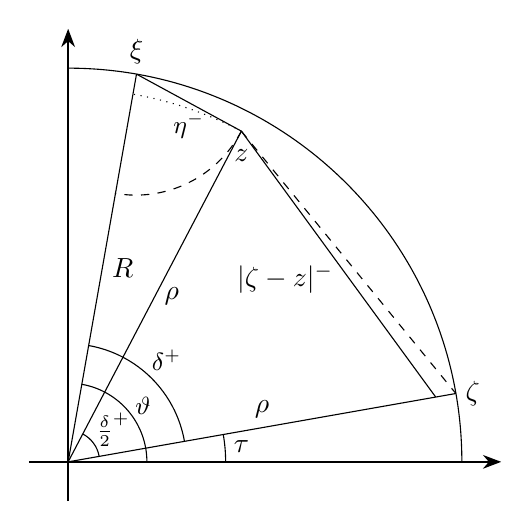
\begin{tikzpicture}
            \coordinate (zeta) at (4.924, 0.868);
            \coordinate (z) at (2.2, 4.2);
            \coordinate (xi) at (0.868, 4.924);
            \coordinate (auxiliary1) at ($(0,0)!0.948!(zeta)$);

            \draw[-{Stealth}, thick] (-0.5, 0) -- (5.5, 0);
            \draw[-{Stealth}, thick] (0, -0.5) -- (0, 5.5);
            \draw[thin] (5,0) arc[start angle=0, end angle=90, radius=5];
            \draw[thin] (0, 0) -- (zeta);
            \draw[thin] (0, 0) -- (xi);
            \draw[thin] (0, 0) -- (z);
            \draw[thin] (z) -- (xi);
            \draw[thin] (z) -- (auxiliary1);
            \draw[dashed, thin] (z) -- (zeta);
            \draw[thin] ($(0,0)!0.08!(zeta)$) arc[start angle=10, end angle=62.35, radius=0.4];
            \draw[thin] ($(0,0)!0.3!(zeta)$) arc[start angle=10, end angle=80, radius=1.5];
            \draw[thin] (2,0) arc[start angle=0, end angle=10, radius=2];
            \draw[thin] (1,0) arc[start angle=0, end angle=80, radius=1];
            \draw[dashed] (z) arc[start angle=-27.65, end angle=-100, radius=1.516];
            \draw[dotted] (z) arc[start angle=62.35, end angle=80, radius=4.741];

            \node[anchor=west] at (zeta) {\(\zeta\)};
            \node[anchor=north] at ([yshift=-3pt] z) {\(z\)};
            \node[anchor=south] at (xi) {\(\xi\)};
            \node[anchor=south] at ($(0,0)!0.5!(zeta)$) {\(\rho\)};
            \node[anchor=north] at ($(z)!0.5!(xi)$) {\small\(\eta^-\)};
            \node[anchor=west] at ($(0,0)!0.5!(xi)$) {\(R\)};
            \node[anchor=west] at ($(z)!0.5!(0,0)$) {\(\rho\)};
            \node[anchor=north] at (0.57,0.75) {\small \(\tfrac{\delta}{2}^+\)};
            \node[anchor=north] at (0.95,0.95) {\small\(\vartheta\)};
            \node[anchor=north] at (1.25,1.55) {\small\(\delta^+\)};
            \node[anchor=north] at (2.2,0.4) {\(\tau\)};
            \node[anchor=east] at ([yshift=-6pt, xshift=-2pt] $(z)!0.5!(zeta)$) {\(|\zeta-z|^-\)};
        \end{tikzpicture}
        \caption{\(\zeta\), \(\xi\), and \(z\) when \(\abs{\vartheta-\tau}>\delta\), with angles and distances marked. The use of \(+\) and \(-\) denote a value more or less (respectively) than the proceeding value.}
        \label{fig:dirichletproblemwithlaplaceequationsolution_secondintegral}
    \end{figure}Since \(\varphi\) is continuous on a compact set \(\partial D(0,R)\), it is bounded by \autoref{lemma:uniformcontinuousovercompactset}, or \(M=\sup_{\qty|\zeta|=R}\abs{\varphi(\zeta)}\) is finite. The Poisson kernel can be rewritten as \[P(\zeta,z)=\frac{R^2-\rho^2}{2\pi\qty|\zeta-z|^2},\]
    where \(\zeta=Re^{i\tau}\) and \(z=\rho e^{i\theta}\), with \(\abs{\vartheta-\tau}>\delta\). Then \(\exists\eta>0\) such that \(\forall z\) with \(|\xi-z|<\eta\), \begin{equation}
        \abs{\theta-\tau}>\frac{\delta}{2}\label{eq:dirichletproblemwithlaplaceequationsolution_constraint1},
    \end{equation} and \begin{equation}
        \rho>\frac{R}{2}\Longrightarrow\eta\leq\frac{R}{2}\label{eq:dirichletproblemwithlaplaceequationsolution_constraint2}
    \end{equation} (these can be arbitrarily chosen for different resulting bounds) as in \autoref{fig:dirichletproblemwithlaplaceequationsolution_secondintegral}. Then, \[|\zeta-z|^2>4\rho^2\sin[2](\frac{\delta}{4})>\frac{1}{2}R^2\qty(1-\cos(\frac{\delta}{2})).\]

    We aim to prove that \(\abs{I_2}<\varepsilon\). Since \(\abs{\varphi\qty(Re^{i\vartheta})-\varphi(\zeta)}<2M\), the condition is satisfied if \(\int_{\abs{\vartheta-\tau}>\delta}\frac{R^2-\rho^2}{\pi R^2\qty(1-\cos(\frac{\delta}{2}))}\dd{\tau}<2\frac{R^2-\rho^2}{R^2\qty(1-\cos(\frac{\delta}{2}))}< \frac{\varepsilon}{2M}\), and from rearrangement, we can significantly tighten the constraint with: \begin{equation}
        R^2-\rho^2<\frac{\varepsilon}{4M}R^2\paren{1-\cos(\frac{\delta}{2})}\Longleftarrow R-\rho<\frac{\varepsilon}{8M}R\paren{1-\cos(\frac{\delta}{2})}.\label{eq:dirichletproblemwithlaplaceequationsolution_constraint3}
    \end{equation}
    From \autoref{fig:dirichletproblemwithlaplaceequationsolution_secondintegral}, it is evident that \(R-\rho<|\xi-z|<\eta\). In order for equation~\eqref{eq:dirichletproblemwithlaplaceequationsolution_constraint1} to be true, we can enforce that \(\abs{\vartheta-\theta}<\frac{\delta}{2}\). In other words \(\abs{\xi-z}^2<R^2+\rho^2-2R\rho\cos(\frac{\delta}{2})\). Obviously, this will be satisfied if \(|\xi-z|^2<\frac{R^2}{2}\paren{1-\cos(\frac{\delta}{2})}<2\rho^2\qty(1-\cos(\frac{\delta}{2}))\). This can be rearranged into \(|\xi-z|<\frac{R\sqrt{2}}{2}\sqrt{1-\cos(\frac{\delta}{2})}=R\sin\qty(\frac{\delta}{4})\) Therefore, we can choose \[\eta=\min\qty[\frac{\varepsilon}{8M}R\paren{1-\cos(\frac{\delta}{2})},R\sin\qty(\frac{\delta}{4}),\frac{R}{2}]>0,\] under which equations \eqref{eq:dirichletproblemwithlaplaceequationsolution_constraint1}, \eqref{eq:dirichletproblemwithlaplaceequationsolution_constraint2} and \eqref{eq:dirichletproblemwithlaplaceequationsolution_constraint3} are satisfied.

    Hence, \(\forall\varepsilon>0\), \(\exists\eta>0\) such that \(\forall z\) such that \(0<\abs{\xi-z}<\eta\), we have \(\abs{\varphi(\xi)-u(z)}<2\varepsilon\). Then equation~\eqref{eq:dirichletproblemwithlaplaceequationsolution_limittoboundary} follows.

    We will now show that \(u(z)\) is unique. Assume that \(v\not\equiv u\) on \(\overline{D(0,R)}\) also solves the problem. Then \(u-v\) is harmonic and vanishes on \(\partial D(0,R)\). By the Poisson Integral Formula (equation~\eqref{eq:poissonintegralformula2}), \(\forall z\in D(0,R)\), \(u(z)-v(z)=\int_0^{2\pi}P(\zeta,z)\paren{u(\zeta)-v(\zeta)}\dd{\tau}=0\). Since \(u-v\) vanishes, we have a contradiction.
\end{proof}
\subsubsection{In Harmonic Analysis}
Consider \(R=1\), \(\zeta=e^{i\tau}\), \(z=\rho e^{i\theta}\) in equation~\eqref{eq:poissonintegralformula2}:
\[u(z)=\int_0^{2\pi}u(\zeta)\frac{1-|z|^2}{\abs{\zeta-z}^2}\dd{\tau}=\int_0^{2\pi}\frac{\qty(1-\rho^2)u\qty(e^{i\tau})\dd{\tau}}{\qty(e^{i\tau}-\rho e^{i\theta})\qty(e^{-i\tau}-\rho e^{-i\theta})}=\int_0^{2\pi}\frac{\qty(1-\rho^2)u\qty(e^{i\tau})\dd{\tau}}{1+\rho^2-2\rho\cos(\theta-\tau)}.\]
If \(u\qty(z)\) is continuous on \(\partial\mathbb{D}\), and therefore \(u\circ\exp(i\tau)\) is periodic over \(2\pi\). Thus, it can be expressed as a Fourier series \[u\qty(e^{i\tau})\sim\sum_{n=-\infty}^\infty a_ne^{in\tau},\qquad a_n=\frac{1}{2\pi}\int_{-\pi}^\pi u\qty(e^{i\tau})e^{-in\tau}\dd{\tau}.\]
This series is not necessarily convergent (hence the usage of "\(\sim\)").
TO BE CONTINUED

Finally, we will demonstrate that real-valued continuous functions satisfying the mean-value property are logically equivalent to being a solution to the Laplace equation. In \autoref{lemma:holomorphicmeanvalueproperty}, we showed that real solutions to the Laplace equation satisfy the mean-value property. Now we will prove the converse.
\begin{theorem}\label{thm:meanvaluepropertysolutionsareharmonic}
    Let \(U\subseteq\mathbb{C}\) be open. Let \(f:U\to\mathbb{R}\) be continuous. \(\forall z_0\in U\), \(\exists\varepsilon>0\) such that \(\overline{D\qty(z_0,\varepsilon)}\subseteq U\), and if \(\forall0<\varepsilon'\le\varepsilon\), \[f(z_0)=\frac{1}{2\pi}\int_0^{2\pi}f\qty(z_0+\varepsilon'e^{it})\ddt,\]
    then \(f\) is harmonic on \(U\).
\end{theorem}
\begin{proof}
    Fix an arbitrary point \(z_0\in U\), along with a corresponding \(\varepsilon>0\) such that the closed disk \(\overline{D(z_0,\varepsilon)}\subseteq U\). Since \(f\in C^0\qty(\partial D(z_0,\varepsilon))\), by \autoref{thm:dirichletproblemwithlaplaceequationsolution}, there exists a unique function \(u(z)\) that is harmonic on \(D(z_0,\varepsilon)\), given by \[u(z)=\int_0^{2\pi}f(\zeta)P\qty(\zeta,z)\dd{\tau},\] which agrees with \(f\) on \(\partial D(z_0,\varepsilon)\).

    Now define \(\psi=f-u \) on \(\overline{D(z_0,\varepsilon)}\). Then \(\psi\) is continuous, satisfies the mean value property, and vanishes on the boundary. By an extension of the Maximum Principle (see the proof of the Maximum Modulus Principle, \autoref{thm:maximummodulus}, which only uses the mean-value property), any such function must be identically zero throughout the disk. Thus, \(f\equiv u\) on \(\overline{D(z_0,\varepsilon)}\), and in particular, \(f\) is harmonic at \(z_0\).

    Since \(z_0\in U\) was arbitrary, it follows that \(f\) is harmonic on \(U\).
\end{proof}
\section{The Theory of Weierstrass}
While Weierstrass' contributions in complex analysis are mainly characterized by his discoveries on uniform convergence, he also characterized entire and \textit{meromorphic functions} and a unique representation of entire functions, as well as his contributions toward the study of \textit{essential singularities}.

To help understand the behavior of non-removable singularities, we will introduce the concept of \textit{Laurent Series}.
\subsection{Laurent Series}
The Laurent Series generalizes the Taylor series to holomorphic functions with isolated singularities. While Taylor series are valid within a disk centered at a point of holomorphy, Laurent series apply to annular regions surrounding a singularity, making them essential for studying functions near non-removable singularities (refer to \autoref{thm:removablesingularitiesriemann}).

We now introduce a fundamental result in complex analysis due to Weierstrass, which formalizes the conditions under which the limit of a sequence of holomorphic functions is itself holomorphic. This theorem not only guarantees the holomorphy of the limit function but also the uniform convergence of its derivatives (its statement was used in the proof of \autoref{thm:hurwitzsimplecase}).
\begin{theorem}[Weierstrass' Uniform Limit Theorem]\label{thm:weierstrassuniformlimit}
    Let \(\cbraces{f_n(z)}_{n\in\mathbb{N}}\) be a sequence of holomorphic functions on an open region \(U\subseteq\mathbb{C}\) that converges uniformly to \(f(z)\) on every compact subset of \(U\). Then \(f(z)\) is holomorphic on \(U\), and \(\forall k\in\mathbb{N}\), the sequence \(\cbraces{f^{(k)}_n(z)}_{n\in\mathbb{N}}\) uniformly converges to \(f^{(k)}(z)\) on all compact subsets of \(U\).
\end{theorem}
\begin{proof}
    By Morera's Theorem (\autoref{thm:morera}) and uniform convergence, the holomorphy of \(f(z)\) follows (refer to equation~\eqref{eq:hurwitzsimplecase_integrallimitswitchforholomorphy} and preceding explanations).

    Following the exact same logic, by \autoref{crl:nthderivativeboundedsupremum}, \(\forall k\in\mathbb{N}\) and for all compact \(K\subset U\) and open \(V\supset K\) relatively compact in \(U\) there exists a finite constant \(c_k>0\) such that
    \[\lim_{n\to\infty}\sup_{z\in K}\abs{f_n^{(k)}(z)-f^{(k)}(z)}\leq c_k\lim_{n\to\infty}\sup_{z\in V}\abs{f_n(z)-f(z)}.\] Since \(\cbraces{f_n(z)}\) is uniformly convergent, the limit on the right-hand side vanishes. Then,
    \[\lim_{n\to\infty}\sup_{z\in K}\abs{f_n^{(k)}(z)-f^{(k)}(z)}=0,\] and therefore \(\qty{f^{(k)}_n(z)}\) uniformly converges on all compact subsets of \(U\).
\end{proof}
The condition of uniform convergence on every compact subset can also be significantly loosened, by the fact demonstrated below:
\begin{lemma}v
    Let \(U\subseteq\mathbb{C}\) be open and bounded, and let \(\qty{f_n(z)}\) be holomorphic on \(U\). Let \(K\subseteq U\) be compact. If \(f_n\rightrightarrows f\) on \(\partial K\), then \(f_n\rightrightarrows f\) on \(K\).
\end{lemma}
\begin{proof}
    By the converse statement of the Cauchy Criterion (\autoref{thm:cauchycriterionuniformconvergence}), \(\forall\varepsilon>0\), \(\exists N\in\mathbb{N}\) such that \(\forall n,m>N\), \[\sup_{z\in\partial K}\qty|f_n(z)-f_m(z)|<\varepsilon.\]
    By the Maximum Modulus Principle (\autoref{thm:maximummodulus}) on \(f_n-f_m\), \[\sup_{z\in\partial K}\abs{f_n(z)-f_m(z)}=\sup_{z\in K}\abs{f_n(z)-f_m(z)}<\varepsilon.\]
    It follows that \(f_n\rightrightarrows f\) on \(K\) by \autoref{thm:cauchycriterionuniformconvergence}.
\end{proof}
\begin{remark}
    From the above result, the uniform convergence on every compact subset in \autoref{thm:weierstrassuniformlimit} can therefore be loosened to the uniform convergence on every simple closed curve.
\end{remark}
We will now study the  Laurent Series. Let \(a\in\mathbb{C}\) and \(\qty{c_n}_{n\in\mathbb{Z}}\subset\mathbb{C}\) be constants. A series in the form of
\begin{equation}\label{eq:laurentseries}
    f(z)=\sum_{n=-\infty}^\infty c_n(z-a)^n
\end{equation}
is a Laurent Series at the point \(a\). The series can be separated into a power series with non-negative exponents, \begin{equation}
    \varphi(z)=\sum_{n=0}^\infty c_n(z-a)^n,\label{eq:laurentseriesnonnegativeexponents}
\end{equation} and a power series with negative exponents, \begin{equation}
    \psi(z)=\sum_{n=1}^{\infty}c_{-n}(z-a)^{-n}.\label{eq:laurentseriesnegativeexponents}
\end{equation} Equation~\eqref{eq:laurentseries} is said to be convergent at \(z=z_0\) if the two power series are both convergent. Let the convergence radius of equation~\eqref{eq:laurentseriesnonnegativeexponents} be \(R=\frac{1}{\varlimsup_{n\to\infty}\sqrt[n]{\abs{c_n}}}\) by the Cauchy--Hadamard Theorem (\autoref{thm:cauchyhadamard}). It follows that the \(\varphi\) is holomorphic on \(D(a,R)\). Let \(\zeta=(z-a)^{-1}\). Then equation~\eqref{eq:laurentseriesnegativeexponents} becomes \(\sum_{n=1}^\infty c_{-n}\zeta^n\). This series converges when \(\abs{\zeta}<\frac{1}{\varlimsup_{n\to\infty}\sqrt[n]{\abs{c_{-n}}}}=\lambda\). Let \(r=\flatfrac{1}{\lambda}\). Then \(\psi(z)\) converges when \(\abs{z-a}>\varlimsup_{n\to\infty}\sqrt[n]{\abs{c_{-n}}}\), or when \(z\in\mathbb{C}\setminus\overline{D(a,r)}\).

If \(R>r\), then \(f\) is convergent on the annulus \(D(a,R)\setminus\overline{D(a,r)}\) and divergent on \(\mathbb{C}\setminus\overline{D(a,R)}\cup D(a,r)\). If \(r=R\), the series diverges possibly everywhere but on \(\partial D(a,r)\). Similar to power series with positive exponents, the convergence on the boundary varies. For example, \(\sum_{\substack{n=-\infty\\n\neq0}}^\infty\frac{z^n}{n^2}\), where \(R=r=1\), converges (absolutely) on \(\partial\mathbb{D}\), whereas \(\sum_{n=-\infty}^\infty z^n\) diverges on all of \(\partial\mathbb{D}\), while \(\sum_{\substack{n=-\infty\\n\neq0}}^\infty\frac{z^n}{n}\) converges (conditionally) on all of \(\partial\mathbb{D}\setminus\qty{1}\) and diverges at \(z=1\). If \(r>R\), then the series is divergent on all of \(\mathbb{C}\). The region \(D(a,R)\setminus\overline{D(a,r)}\) is known as the \textit{annulus of convergence}. \(f(z)\) in equation~\eqref{eq:laurentseries} is holomorphic over this annulus. \(\varphi(z)\) is known as the \textit{holomorphic part} of \(f(z)\), and \(\psi(z)\) is known as the \textit{principal part} of the Laurent Series. The properties of the convergence disk in Abel's Theorem (\autoref{thm:abelradius}) can be generalized to Laurent Series. \(f\) is absolutely convergent on the annulus and is uniformly convergent on every compact subset of it.
\begin{theorem}\label{thm:laurentexpansionofholomorphicfunction}
    Let \(V=\cbraces{z\in\mathbb{C}}{r<\abs{z-a}<R}\) for some \(0\leq r<R\leq\infty\). Let \(f\) be holomorphic on \(V\). Then \(f\) has the unique \textit{Laurent expansion} \begin{equation}
        f(z)=\sum_{n=-\infty}^\infty c_n(z-a)^n\label{eq:laurentexpansionofholomorphicfunction_statement}
    \end{equation} when \(z\in V\), where \(c_n=\frac{1}{2\pi i}\oint_{\gamma}\frac{f(\zeta)\ddzeta}{(\zeta-a)^{n+1}}\), where \(\gamma\subset V\) is a simple closed curve enclosing \(a\).
\end{theorem}
\begin{proof}
    \begin{figure}
        \centering
        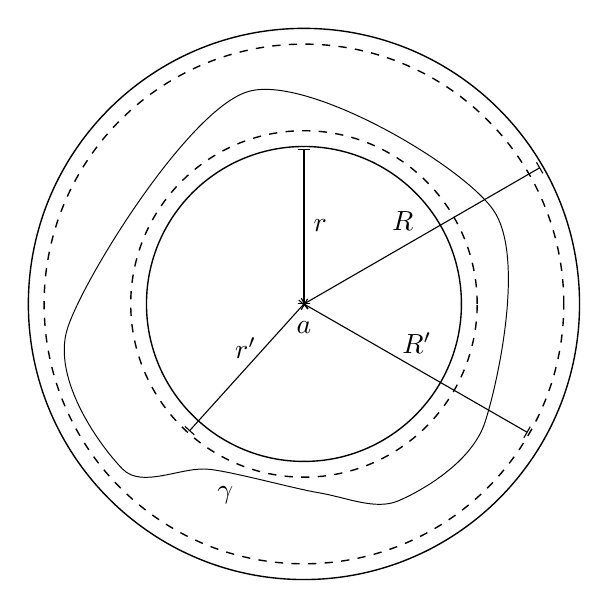
\begin{tikzpicture}
            \draw[line width=0.35] plot[smooth cycle] coordinates {
                    (-3,-0.3) (-2.3,-2.1) (-1.2,-2.1) (0.2,-2.4) (1.2,-2.5) (2.3,-1.5) (2.4,1.2) (-0.7,2.7)
                };
            \draw[line width=0.5] (3.5,0) arc[start angle=0, end angle=360, radius=3.5];
            \draw[line width=0.5, dashed] (3.3,0) arc[start angle=0, end angle=360, radius=3.3];
            \draw[line width=0.5] (2,0) arc[start angle=0, end angle=360, radius=2];
            \draw[line width=0.5, dashed] (2.2,0) arc[start angle=0, end angle=360, radius=2.2];
            \draw[thin, |-|, line cap=round, shorten >=1pt] (0,0) -- (3.03,1.75) node[midway, anchor=south east, yshift=-2pt] {\(R\)};
            \draw[thin, |-|, line cap=round, shorten >=1pt] (0,0) -- (0,2) node[midway, right] {\(r\)};
            \draw[thin, |-|, line cap=round, shorten >=1pt] (0,0) -- (2.87,-1.65) node[midway, anchor=south, yshift=2pt] {\(R'\)};
            \draw[thin, |-|, line cap=round, shorten >=1pt] (0,0) -- (-1.48,-1.64) node[midway, anchor=south] {\(r'\)};

            \node[anchor=north] at (0,-0.1) {\(a\)};
            \node[anchor=north] at (-1,-2.2) {\(\gamma\)};
        \end{tikzpicture}
        \caption{The annulus \(V\), with \(\gamma_1\), \(\gamma_2\), and \(\gamma\).}
        \label{fig:laurentexpansionofholomorphicfunction}
    \end{figure}By the openness of \(V\), there exist two circles \(\gamma_1\subset V\) with radius \(r'\) and \(\gamma_2\subset V\) with radius \(R'\) centered at \(a\) such that \(\gamma\) encloses \(\gamma_1\) and \(\gamma_2\) encloses \(\gamma\) both without intersection. Let \(W=\cbraces{z\in V}{r'<|z-a|<R'}\) and \(z\in W\) be arbitrary. By the Cauchy--Goursat Integral Formula (\autoref{thm:cauchygoursatformula}), \[f(z)=\frac{1}{2\pi i}\qty(\int_{\gamma_2}\frac{f(\zeta)\ddzeta}{\zeta-z}-\int_{\gamma_1}\frac{f(\zeta)\ddzeta}{\zeta-z}).\]
    \(\forall\zeta\in\gamma_1\) (or \(|\zeta-a|=r'\)), \(\abs{\zeta-a}<\abs{z-a}\) and therefore, \(\frac{\abs{\zeta-a}}{\abs{z-a}}<1\). It follows that \begin{equation}
        \frac{1}{\zeta-z}=-\frac{1}{(z-a)\qty(1-\dfrac{\zeta-a}{z-a})}=-\sum_{n=0}^\infty\frac{\qty(\zeta-a)^n}{\qty(z-a)^{n+1}}\label{eq:laurentexpansionofholomorphicfunction_kernelexpansioninside}
    \end{equation} is uniformly convergent with respect to \(\zeta\). Similarly, \(\forall\zeta\in\gamma_2\), \(\abs{\zeta-a}>\abs{z-a}\Leftrightarrow\frac{\abs{z-a}}{\abs{\zeta-a}}<1\), and it follows that \begin{equation}
        \frac{1}{\zeta-z}=\frac{1}{(\zeta-a)\qty(1-\dfrac{z-a}{\zeta-a})}=\sum_{n=0}^\infty\frac{\qty(z-a)^n}{\qty(\zeta-a)^{n+1}}\label{eq:laurentexpansionofholomorphicfunction_kernelexpansionoutside}
    \end{equation} is uniformly convergent with respect to \(\zeta\). By the boundedness of \(f\) on \(\gamma_1\) and \(\gamma_2\) from holomorphy on a compact set, and from the Weierstrass \(M\)--Test, we get that \begin{equation}
        f(z)=\frac{1}{2\pi i}\qty(\sum_{n=0}^\infty\int_{\gamma_2}\frac{(z-a)^n}{(\zeta-a)^{n+1}}f(\zeta)\ddzeta+\sum_{n=1}^\infty\int_{\gamma_1}\frac{(\zeta-a)^{n-1}}{(z-a)^{n}}f(\zeta)\ddzeta).\label{eq:laurentexpansionofholomorphicfunction_finalstep}
    \end{equation}
    By the Cauchy--Goursat Integral Theorem (\autoref{thm:cauchygoursattheorem}), for a given \(n\), \[\int_{\gamma_2^+\cup\gamma^-}\frac{f(\zeta)\ddzeta}{(\zeta-a)^n}=0,\quad\int_{\gamma^+\cup\gamma_1^-}f(\zeta)(\zeta-a)^n\ddzeta=0.\]
    In other words, the integrals in equation~\eqref{eq:laurentexpansionofholomorphicfunction_finalstep} are the same as on \(\gamma\). Hence, we get that \[f(z)=\sum_{n=0}^\infty c_n(z-a)^n+\sum_{n=1}^\infty c_{-n}(z-a)^{-n}=\sum_{n=-\infty}^\infty c_n(z-a)^n.\]
    The constants \(\qty{c_n}_{n\in\mathbb{Z}}\) are also unique in the expansion. For the sake of contradiction, assume there exists another set of constants \(\qty{c'_n}_{n\in\mathbb{Z}}\) such that \begin{equation}
        f(z)=\sum_{n=-\infty}^\infty c'_n(z-a)^n,\label{eq:laurentexpansionofholomorphicfunction_uniquenessstatement}
    \end{equation}
    where \(z\in V\) and the series is uniformly convergent on \(\gamma\). Let \(m\in\mathbb{Z}\) be arbitrary. By the Cauchy--Goursat Differentiation Formula (\autoref{thm:cauchydifferentiationformula}), \[\int_{\gamma}(z-a)^k\ddz=\begin{cases}
            0                     & k\geq0   \\
            2\pi i\dv[-k-1]{z}(1) & k\leq -1
        \end{cases}=\begin{cases}
            0      & k\neq-1 \\
            2\pi i & k=-1    \\
        \end{cases}.\]
    Multiplying equation~\eqref{eq:laurentexpansionofholomorphicfunction_uniquenessstatement} by \((z-a)^{-m-1}\) and from integrating over \(\gamma\), we get that \[\int_\gamma\frac{f(z)\ddz}{(z-a)^{m+1}}=\int_{\gamma}\sum_{n=-\infty}^\infty c'_n(z-a)^{n-m-1}\ddz\Longleftrightarrow 2\pi ic_m=\sum_{n=-\infty}^\infty c'_n\int_{\gamma}(z-a)^{n-m-1}\ddz=2\pi ic'_m,\]
    and we have a contradiction, implying uniqueness.
\end{proof}
\subsection{Isolated Singularities}
An \textit{isolated singularity} of a complex function is a point \(a\in\mathbb{C}\) where a function \(f\) is holomorphic on some open punctured neighborhood of \(a\) (namely, for some \(r>0\), the punctured disk \(D^*(a,r)\)), but not necessarily defined or holomorphic at \(a\) itself. The nature of this isolated singularity is characterized by the principal part \(\psi(z)\) (let \(\varphi(z)\) be the holomorphic part) of the Laurent series of \(f\) at the point \(a\). Specifically, we can analyze the behavior of \(f(z)\) as \(z\to a\).
\begin{enumerate}
    \item\label{itm:isolatedsingularities_removable} If \(\lim_{z\to a}f(z)\) exists and is finite, then \(z=a\) is a removable singularity and can be analytically continued to \(D(a,r)\) by \autoref{thm:removablesingularitiesriemann}. Consequently, \(f(z)\) has a convergent Taylor expansion and the principal part of its Laurent expansion vanishes, and \(f(z)=\varphi(z)\).
    \item\label{itm:isolatedsingularities_pole} If \(\lim_{z\to a}f(z)=\infty\), then \(z=a\) is a \textit{pole} of \(f\) (from the stereographic projection and the Riemann sphere, the \(\infty\) is a single point in \(\riemannsphere\), and approaching \(\infty\) does not distinguish between different directions, unlike the use of \(+\infty\) and \(-\infty\)). \begin{theorem}\label{thm:isolatedsingularities_pole_laurentexpansion}
              The condition \(\lim_{z\to a}f(z)=\infty\) is equivalent to there being a finite number of nonzero \(c_{-n}\)'s, where \(n\in\mathbb{N}\).
          \end{theorem}
          In other words the principal part of \(f\) is equal to \[\psi(z)=\frac{c_{-1}}{z-a}+\cdots+\frac{c_{-m}}{(z-a)^m}\quad c_{-m}\neq0\] for some \(m\in\mathbb{N}\). Therefore, \(f(z)=\varphi(z)+\psi(z)=\sum_{n=-m}^\infty c_n(z-a)^n=\frac{g(z)}{(z-a)^m}\) on the punctured disk \(D^*(a,r)\), where \(g(z)=\sum_{n=0}^\infty c_{n-m}(z-a)^n\) is holomorphic on \(D(a,r)\) and does not attain a zero at \(z=a\). Then \(f(z)\) has a pole at \(z=a\) with order \(m\). If \(m=1\), the pole is also called a \textit{simple pole}.
          \begin{proof}
              Obviously, under the assumption of a finite, nonempty number of non-negative terms in the principal part of the Laurent expansion coefficients, \(\lim_{z\to a}f(z)\to\infty\). Now we will prove the converse. Let \(g(z)=\frac{1}{f(z)}\). Then \(\lim_{z\to a}g(z)=0\). There exists a \(\delta>0\) such that \(f\) is nonzero on \(D^*(a,\delta)\). Then \(g(z)\) is holomorphic on \(D^*(a,\delta)\) and has a removable singularity at \(z=a\). By \autoref{thm:removablesingularitiesriemann}, \(g\) can be analytically continued to \(D^*(a,\delta)\). Let the multiplicity of the zero at \(z=a\) be \(m\). Then \(g(z)=\phi(z)(z-a)^m\), where \(\phi(z)\) is holomorphic and nonzero at \(z=a\). Then there exists a \(\delta'>0\) such that \(\phi\) is nonzero on \(D(a,\delta')\). It follows that \(\frac{1}{\phi}\) is holomorphic and nonzero on \(D(a,\delta')\). We can then write its Taylor expansion as \[\frac{1}{\phi(z)}=c_{-m}+c_{1-m}(z-a)+\cdots,\]
              where \(c_{-m}\neq0\). It follows that \[f(z)=\frac{1}{g(z)}=\frac{(z-a)^{-m}}{\phi(z)}={c_{-m}}(z-a)^{-m}+c_{1-m}(z-a)^{1-m}+\cdots+c_0+\cdots.\]
              By the uniqueness of the Laurent series (by \autoref{thm:laurentexpansionofholomorphicfunction}), the conclusion follows.
          \end{proof}
    \item\label{itm:isolatedsingularities_essential} If \(\lim_{z\to a}f(z)\) is nonexistent, then \(a\) is known as an \textit{essential singularity}.
          \begin{example}\label{ex:isolatedsingularities_essential_exp1z}
              The function \(e^{\frac{1}{z}}\) has an essential singularity at \(z=0\).
          \end{example}
          \begin{proof}
              Observe that \(\lim_{\substack{z\to 0\\z\in\mathbb{R}_{>0}}}=\infty\). Similarly, \(\lim_{\substack{z\to0\\z\in\mathbb{R}_{<0}}}=0\), and \(\lim_{\substack{z\to0\\z\in i\mathbb{R}_{>0}}}\) is divergent.
          \end{proof}
          The implication on its Laurent expansion at \(a\) is:
          \begin{theorem}
              The necessary and sufficient for \(\lim_{z\to a} f(z)\) to not exist is that infinitely many of \(c_{-n}\) (where \(n\in\mathbb{N}\)) are nonzero.
          \end{theorem}
          This follows by elimination from the established trichotomy; if the limit as \(z\to a\) does not exist, then the singularity is neither removable nor a pole (results from \ref{itm:isolatedsingularities_removable} and \ref{itm:isolatedsingularities_pole}). Similar logic can be applied to the coefficients of the Laurent expansion.

          Indeed, in \autoref{ex:isolatedsingularities_essential_exp1z}, the Laurent expansion is equal to:
          \[e^{\frac{1}{z}}=\sum_{n=0}^\infty\frac{z^{-n}}{n!},\]
          which has infinitely many nonzero coefficients of negative powers.
\end{enumerate}
A function with an essential singularity exhibits striking behavior. We will first introduce the following famous result.
\begin{theorem}[Weierstrass--Casorati Theorem]\label{thm:weierstrasscasorati}
    Let \(a\in\mathbb{C}\) and \(U\subseteq\mathbb{C}\) be open. Suppose \(f:U\setminus\qty{a}\to\mathbb{C}\) is holomorphic with an essential singularity at \(a\). Then the set of values that \(f\) attains on any open punctured neighborhood of \(a\) is dense. In other words, \(\forall\varepsilon,\delta>0\), \(\forall w\in\mathbb{C}\), \(\exists z\in D^*(a,\delta)\) such that \(|f(z)-w|<\varepsilon\).
\end{theorem}
\begin{proof}
    Assume for the sake of contradiction that \(\exists\varepsilon,\delta>0\), and \(\exists w\in\mathbb{C}\) such that \(\forall z\in D^*(a,\delta)\), \(|f(z)-w|>\varepsilon\). Define the auxiliary function \(g(z)=\frac{f(z)-w}{z-a}\), which is holomorphic and non-vanishing on the punctured neighborhood of \(a\). Since as \(z\to a\), \(g(z)\to\infty\), it follows that \(g(z)\) has a pole at \(a\). Let the order of the pole be \(m\in\mathbb{N}\). By \autoref{thm:isolatedsingularities_pole_laurentexpansion}, \(g(z)\) has the Laurent expansion of \[\frac{c_{-m}}{(z-a)^m}+\cdots c_0+c_1(z-a)+\cdots\]
    for some \(m\in\mathbb{N}\). It follows that \[f(z)=\frac{c_{-m}}{(z-a)^{m-1}}+\cdots+c_{-1}+w+c_0(z-a)+\cdots.\] If \(m=1\), then \(f\) has a removable singularity at \(a\). If \(m\geq2\), then \(f\) has a pole at \(a\). Hence, we have a contradiction.
\end{proof}
In \chpref{sec:differentialgeometry}, we will prove a profound generalization of this result (\autoref{thm:greatpicard}), which was first proved by Émile Picard in 1879: \textit{the image of any open punctured neighborhood of an essential singularity of a holomorphic function will attain every value in \(\mathbb{C}\), except for at most one possible exception, infinitely often}.
\subsubsection{At the \texorpdfstring{\(\infty\)}{Infinity} Point}
Given the one-point compactification of \(\mathbb{C}\) into the Riemann sphere \(\riemannsphere\), we can now define and analyze the behavior of functions near the point at infinity. Similar to the classification of isolated singularities in \(\mathbb{C}\), we can classify \(\infty\) as a removable singularity, a pole, or an essential singularity of a holomorphic function.

Let \(f:\mathbb{C}\setminus\overline{D(0,R)}\to\mathbb{C}\) be holomorphic for some \(R>0\). Then \(z=\infty\) is an \textit{isolated singularity} of \(f\). To analyze the nature of the singularity, let \(\zeta=\frac{1}{z}\). We define a new function \(g(\zeta)=f\qty(\frac{1}{\zeta})=f(z)\), which is holomorphic on \(D^*\qty(0,\frac{1}{R})\). Then at \(\zeta=0\), \(g(\zeta)\) has the Laurent expansion of \[g(\zeta)=\sum_{n=-\infty}^\infty c_n\zeta^n=\sum_{n=0}^\infty c_{n}\zeta^n+\sum_{n=1}^\infty c_{-n}\zeta^{-n}=\varphi(\zeta)+\psi(\zeta),\]
where \(\varphi\) and \(\psi\) are the holomorphic and principal parts of \(g\), respectively. Let \(\tilde{\varphi}(z)=\varphi\qty(\frac{1}{z})\), \(\tilde{\psi}(z)=\psi\qty(\frac{1}{z})\). At \(z=0\), \(f\) then has the Laurent expansion of \[f(z)=\sum_{n=-\infty}^\infty c_nz^{-n}=\sum_{n=0}^\infty c_nz^{-n}+\sum_{n=1}^\infty c_{-n}z^n=\tilde{\varphi}(z)+\tilde{\psi}(z).\]

The classification of the singularity at \(\infty\) is then reduced to the classification of the singularity of \(g\) at \(0\):
\begin{enumerate}
    \item If \(z=\infty\) is a removable singularity of \(f(z)\), then \(f(z)\) has the form \[f(z)=c_0+\frac{c_1}{z}+\frac{c_2}{z^2}+\frac{c_3}{z^3}+\cdots.\]
    \item If \(z=\infty\) is a pole of \(f(z)\) with degree \(m\in\mathbb{N}\), then \(f(z)\) can be written as \[f(z)=c_{-m}z^m+c_{1-m}z^{m-1}+\cdots c_0+\frac{c_1}{z}+\cdots,\] where \(c_{-m}\neq0\).
    \item If \(z=\infty\) is an essential singularity of \(f(z)\), then \(f(z)\) can be expanded as \[f(z)=\sum_{n=-\infty}^\infty c_{-n}z^n,\]
    where \(\forall N\in\mathbb{N}\), \(\exists n>N\) such that \(c_{-n}\neq0\) (infinitely many coefficients of \(\tilde{\psi}\) are nonzero). 
\end{enumerate}
\begin{example}
    The function \(z\mapsto\frac{1}{z}\) has a removable singularity at \(z=\infty\), the function \(z\mapsto z^2\) has a pole at \(z=\infty\), and \(z\mapsto e^z\) has an essential singularity at \(z=\infty\).
\end{example}
\begin{example}[Cauchy's Integral Formula on the Exterior]\label{ex:cauchygoursatformulaexterior}
    Let \(\gamma\subset\mathbb{C}\) be a simple closed curve, and suppose that \(f:\mathrm{ext}(\gamma)\to\mathbb{C}\) is holomorphic and continuous on \(\overline{\mathrm{ext}(\gamma)}=\mathbb{C}\setminus\mathrm{int}(\gamma)\), where \(\mathrm{int}\) and \(\mathrm{ext}\) respectively denote the interior and exterior as in \autoref{thm:jordancurve}.
    \begin{enumerate}
        \item If \(f\) has a removable singularity at \(\infty\), or if \(w=\lim_{z\to\infty} f(z)\) exists and is finite, then \(\forall z\in\mathbb{C}\setminus\gamma\), \[\frac{1}{2\pi i}\int_\gamma\frac{f(\zeta)}{\zeta-z}\ddzeta=\begin{cases}
            w&z\in\mathrm{int}(\gamma)\\
            w-f(z)&z\in\mathrm{ext}(\gamma)
        \end{cases}.\]
        \item If \(\gamma\) encloses the origin, then \(\forall z\in\mathbb{C}\setminus\gamma\), then \begin{equation}
            \frac{1}{2\pi i}\int_\gamma\frac{zf(\zeta)}{z\zeta-\zeta^2}\ddzeta=\begin{cases}
            0&z\in\mathrm{int}(\gamma)\\
            f(z)&z\in\mathrm{ext}(\gamma)\label{eq:cauchygoursatformulaexteriorpart2}
        \end{cases}.
        \end{equation}
    \end{enumerate}
\end{example}
\begin{proof}
    \begin{enumerate}
        \item By the compactness of \(\gamma\), it can be completely contained within a sufficiently large disk centered at the origin (\(\gamma\in D(0,R)\)). Then by applying \autoref{thm:cauchygoursatformula} or \autoref{thm:cauchygoursattheorem} on the set \(D(0,R)\cap\mathrm{ext}(\gamma)=D(0,R)\setminus\overline{\mathrm{int}(\gamma)}\), we get that \[\frac{1}{2\pi i}\int_{\partial D(0,R)}\frac{f(\zeta)}{\zeta-z}\ddzeta=\frac{1}{2\pi i}\int_\gamma\frac{f(\zeta)}{\zeta-z}\ddzeta+\begin{cases}
        0&z\in\mathrm{int}(\gamma)\\
        f(z)&z\in D(0,R)\cap\mathrm{ext}(\gamma)
    \end{cases}.\]
    By letting \(R\to\infty\) and letting \(\zeta=Re^{i\theta}\), we get that \[\frac{1}{2\pi i}\int_\gamma\frac{f(\zeta)}{\zeta-z}\ddzeta=\frac{1}{2\pi}\lim_{R\to\infty}\int_0^{2\pi}\frac{f\qty(Re^{i\theta})}{1-\frac{z}{Re^{i\theta}}}\dd{\theta}-\begin{cases}
        0&z\in\mathrm{int}(\gamma)\\
        f(z)&z\in\mathrm{ext}(\gamma)
    \end{cases}.\]
    By the continuity of \(f\) on \(\partial D(0,R)\), it attains its maximum \(M\). For sufficiently large \(R\), \(\abs{1-\frac{z}{Re^{i\theta}}}\) attains a positive minimum. Then the integrand is uniformly bounded with respect to \(R\) under \(\theta\), and we can commute the limit with the integral. Hence, \begin{align*}
        \frac{1}{2\pi i}\int_\gamma\frac{f(\zeta)}{\zeta-z}\ddzeta&=\frac{1}{2\pi}\int_0^{2\pi}\frac{w}{1-\lim_{R\to\infty}\frac{z}{Re^{i\theta}}}\dd{\theta}-\begin{cases}
        0&z\in\mathrm{int}(\gamma)\\
        f(z)&z\in\mathrm{ext}(\gamma)
    \end{cases}\\&=\begin{cases}
        w&z\in\mathrm{int}(\gamma)\\
        w-f(z)&z\in\mathrm{ext}(\gamma)
    \end{cases},
    \end{align*} as expected.
    \item Under the partial fraction decomposition of equation~\eqref{eq:cauchygoursatformulaexteriorpart2}, we get that \[I=\int_\gamma\frac{zf(\zeta)}{z\zeta-\zeta^2}\ddzeta=\int_\gamma\qty(\frac{f(\zeta)}{\zeta}-\frac{f(\zeta)}{\zeta-z})\ddzeta\]
    \end{enumerate}
\end{proof}
\subsection{Entireness and Meromorphy}
We have previously defined the concept of an entire function in \chpref{sec:complexdifferentiation}. Let \(f\) be entire with the unique Taylor expansion \(\sum_{n=0}^\infty c_nz^n\). Since \(z=\infty\) is an isolated singularity, by the uniqueness of the Laurent expansion, the expansion at \(z=0\) has the same form as the expansion at \(z=\infty\). We will now analyze the implications on the entire function \(f\) given an isolated singularity.
\begin{enumerate}
    \item If \(f(z)\) has a removable singularity at \(z=\infty\), then \(f\) is constant.
    \begin{proof}
        Let \(z=\frac{1}{\zeta}\), \(g(\zeta)=f\qty(\frac{1}{\zeta})\), which has a removable singularity at \(\zeta=0\). By \autoref{thm:removablesingularitiesriemann}, \(g\) can be analytically continued to all of \(\mathbb{C}\), especially at \(\zeta=0\). Let \(w=g(0)\). Then, \(\forall\varepsilon>0\), \(\exists\delta>0\) such that \(\forall\zeta\in D(0,\delta)\), \(|g(\zeta)-w|<\varepsilon\). It follows that \(\forall |z|>\frac{1}{\delta}\), \(\abs{f(z)}<|w|+\varepsilon\), and is bounded. For the complement, \(\forall z\in \overline{D\qty(0,\frac{1}{\delta})}\), \(f(z)\) is continuous on a compact set, and by \autoref{thm:continuousfunctionboundedoncompact}, is also bounded.

        Then by Liouville's Theorem (\autoref{thm:liouville}), \(f\) is constant. 
    \end{proof}
    \item If \(f(z)\) has a pole at \(z=\infty\), then 
\end{enumerate}
\begin{definition}[Meromorphic Function]
    A
\end{definition}
\subsection{The Residue Theorem}\label{sec:cauchyresiduetheorem}
\subsection{The Group of Holomorphic Automorphisms on \texorpdfstring{\(\mathbb{C}\)}{the complex plane} and \texorpdfstring{\(\riemannsphere\)}{the riemannsphere}}
\section{A Taste of Riemannian Geometry}
One of the goals of higher mathematics is the generalization and unification of existing concepts. As we have seen, traditional complex analysis is the generalization of calculus to functions of complex variables, while the unique properties of holomorphic functions do not correspond to any of those in classical calculus. The Residue Theorem in \chpref{sec:cauchyresiduetheorem} is a result from a generalization that can be applied to real-valued integrals.

More contemporary results in complex analysis are also where many different branches of mathematics, including topology, geometry, number theory, group theory, and linear algebra, coalesce.
\section{Differential Geometry}\label{sec:differentialgeometry}
\begin{theorem}[Picard's Great Theorem]\label{thm:greatpicard}
    
\end{theorem}
\section{Some Differences in Multivariable Complex Analysis}
\end{document}